\documentclass{article} % For LaTeX2e
\usepackage{nips15submit_e,times}
%\usepackage{hyperref}
\usepackage{url}
\usepackage{amsmath}
\usepackage{amssymb}
\usepackage{tikz,pgfplots,adjustbox,graphicx}
\usepackage{subcaption}
\usepackage{todonotes}
\usepackage{float}
\usepackage{wrapfig}
\definecolor{crimson}{rgb}{0.6,0,0}
\definecolor{red}{HTML}{FF4136}
\definecolor{green}{HTML}{2ECC40}
\setlength{\parindent}{1cm}
\numberwithin{figure}{section}
%\documentstyle[nips14submit_09,times,art10]{article} % For LaTeX 2.09

\usepackage{xcolor}
\definecolor{nicepurple}{HTML}{B10DC9}
\definecolor{niceblue}{HTML}{0074D9}
\usepackage[colorlinks=true,linkcolor=niceblue,citecolor=nicepurple]{hyperref}

\title{Variational Auto Encoder Latent Space Activity and Visualization}


\author{
Jesse Bettencourt\\
Department of Mathematics\\
University of Toronto\\
Toronto, ON \\
\texttt{jessbett@math.toronto.edu} \\
\And
Matt Craddock\\
Department of Computer Science\\
University of Toronto\\
Toronto, ON \\
\texttt{matt.craddock@mail.utoronto.ca} \\
}

% The \author macro works with any number of authors. There are two commands
% used to separate the names and addresses of multiple authors: \And and \AND.
%
% Using \And between authors leaves it to \LaTeX{} to determine where to break
% the lines. Using \AND forces a linebreak at that point. So, if \LaTeX{}
% puts 3 of 4 authors names on the first line, and the last on the second
% line, try using \AND instead of \And before the third author name.

\newcommand{\fix}{\marginpar{FIX}}
\newcommand{\new}{\marginpar{NEW}}

\renewcommand{\L}{\mathcal{L}}

\nipsfinalcopy % Uncomment for camera-ready version

\begin{document}
\maketitle

\begin{abstract}
In this project we implement a Variational Auto Encoder (VAE) in Tensorflow. We compare experimental results for modifications to the VAE, including Importance Weighting, Batch Normalization, and Warm-Up. In particular, we consider how these additional methods affect the training rate and latent dimension activity. Finally, we demonstrate latent visualization techniques available with VAEs.
\end{abstract}

\section{Introduction to Variational Autoencoders}

Variational Auto Encoders (VAEs) were introduced by Kingma \& Welling 2013 as generative analogues to the standard deterministic auto encoder \cite{Kingma2013}. As with deterministic auto encoders, VAEs pair a bottom-up inference network called an encoder with a top-down generative network called a decoder. 
\par VAEs employ a probabilistic interpretation of these encoder and decoder networks. We assume that our data set $\{x^{(i)}\}_{i=1}^N$ is composed of $N$ i.i.d. samples of some variable $x$. Further, we assume that the data were generated by a random process with continuous latent variable $z$. So we have that our data $x$ was generated by some conditional distribution $p_\theta(x|z)$, where $p_\theta$ is a probability distribution with parameters $\theta$. This provides a probabilistic interpretation of the decoder network, where given a latent variable or ``code`` $z$ we generate a sample $x$ in the data space. Similarly, the role of the encoder would be to take a sample $x$ from data space and give us a latent $z$ sampled from the posterior density distribution $p_\theta(z|x)$. 
\par However, this is where problems arise in the probabilistic interpretation. It is common that the posterior density distribution $p_\theta(z|x)$ is intractable. In order to learn an encoder-decoder network pair, VAEs instead learn a different inference model, $q_\phi(z|x)$, which approximates the true, intractable posterior distribution. Note that our approximate inference model, the encoder distribution, has parameters $\phi$ distinct from the $\theta$ of the true posterior and decoder network. Training a VAE will amount to jointly learning these these parameters.
\par Variational auto encoders are further characterized by their training criterion. Instead of learning an often intractable log-likelihood, the training objective $\L(x)$ is a tractable lower bound to the log-likelihood:


\begin{align}
  \log p_\theta(x)\geq \mathbb{E}_{q_\phi(z|x)}\left[\log\frac{p_\theta(x,z)}{q_\phi(z|x)}\right]=-\L(x)\\
  \L(x)=D_{KL}\left(q_\phi(z|x)||p_\theta(z)\right)-\mathbb{E}_{q_\phi(z|x)}\left[\log{p_\theta(x|z)}\right]
  \label{eq:VAEOBJECTIVE}
\end{align}
 
 Where $D_{KL}$ is the Kullback-Leibler divergence. It will be useful later to directly identify the two components of our objective. The reconstruction error term $\mathbb{E}_{q_\phi(z|x)}\left[\log{p_\theta(x|z)}\right]$ is present in deterministic auto encoders, and represents the likelihood that the input data would be reconstructed by the model. The variational regularization term $D_{KL}\left(q_\phi(z|x)||p_\theta(z)\right)$ represents the KL-divergence between the encoder-induced latent distribution and the true prior on the latent distribution. This term encourages our approximate posterior $q_\phi(z|x)$ to be close to $p_\theta(z)$.
\par Finally, one last detail to discuss in the process of training a VAE is the reparametrization trick. Since the reconstruction error term is estimated by sampling $z\sim q_\phi(z|x)$, using gradient training methods through the sampling process is problematic. To address this, Kingma \& Welling describe an alternative method for generating the samples, simply to let $z=g_\phi(x,\epsilon)$ be a deterministic function of $\phi$ and $\epsilon$ be some independent noise.
\par For example, in our implementation, which we will soon describe in detail, we assume that the true posterior distribution can be approximated by a multivariate Gaussian with diagonal covariance. Therefore we let $q_\phi(z|x)=\mathcal{N}(z;\mu,\sigma^2 I)$. So the outputs of our encoder network are the $\mu$ and $\sigma$ of our approximate posterior. Now in order to train with gradient methods, we reparameterize as described, letting $z=\mu + \sigma\epsilon$ where $\epsilon \sim \mathcal{N}(0,1)$.

\section{Implementing Variational Autoencoders}
%In this section we will detail methods for VAE implementation and their effect on the learning rate.\\ \todo{Is this necessary?}
\subsection{Network Architecture}
Each of the following methods were included into what will we call the `Vanilla VAE'. The network architecture for the Vanilla VAE and all additional methods is similar to the architecture introduced in the Section $3$ example of Auto-Encoding Variational Bayes \cite{Kingma2013}.
\par The encoder and decoder networks are symmetric, shallow, fully-connected neural networks, namely Multi Layer Perceptrons (MLP). Both feature two deterministic layers each with $200$ dimensions (or nodes) per layer. A stochastic, or latent, layer with dimensions $n_z$ receives the output from the final deterministic layer.  In the nodes of the hidden layers the activation is determined by the softplus function, $\ln{\left(1+e^x\right)}$.
\par Practically, the probabilistic encoder network takes data from the input space and encodes a representation into a latent space with dimension $n_z$. In particular, the latent representation, $q_\phi(z|x)=\mathcal{N}(z;\mu,\sigma^2 I)$ is a Gaussian distribution over the possible latent values of $z$ from which data $x$ could have been generated. The probabilistic decoder network takes a latent representation and produces a distribution ${p_\theta(x\mid z)}$ over possible data values $x$ generated by $z$.
\par We implement this network and the following additional methods in Tensorflow. Our implementation follows from examples in Tensorflow and Theano \cite{Sonderby2016,Metzen2015,Ahuja}. In all examples we are training on the MNIST handwritten digit data set. We learn the MLP weights and bias parameters, representing the $\phi$ and $\theta$ distribution parameters, with Adam optimization minimizing $\L(x)$ with parameters $\beta_1 = 0.9, \beta_2 = 0.9, \epsilon = 10^{-4}$ a batch size of $100$, and learning rate of $0.001$, trained for $300$ epochs.


\subsection{Xavier Initialization}
All parameters in the MLP were initialized with the Xavier-Glorot method outlined in \cite{Glorot2010}. Xavier-Glorot initialization is shown to improve learning in deep networks by establishing an effective range for initial values. In general, especially for deep networks, there is an initial value trade-off. If the initial weights are too small then the signal magnitude will decrease through the layers and and the influence will tend too small to be useful. If the weights are too large then the signal will grow as it passes through the layers and will tend to be too large to be representative.
\par Xavier-Glorot initialization addresses this trade-off by sampling initialization weights from a Gaussian distribution with zero mean and variance as a function of the network connections for the node. The variance for weight $w$  of a neuron is given as a function of the number of neurons feeding into it $n_{in}$ and the number of neurons the result feeds to $n_{out}$. The function is defined to be $\text{Var}(w) = \frac{2}{n_{in}+n_{out}}$.


\subsection{Decoder Distribution}

As mentioned previously, the probabilistic decoder network takes a latent representation $z$ and produces a distribution over possible data values, ${p_\theta(x\mid z)}$. In our initial description of the network architecture we specified that output of the encoder MLP is Gaussian, but we made no specification to the decoder output distribution.
\par Two choices for decoder distributions, Gaussian and Bernoulli, were outlined in \textit{Auto-Encoding Variational Bayes}, where the authors suggest that the choice of preferred decoder distribution depends on the type of data \cite{Kingma2013}. 

\subsubsection{Gaussian Decoder and Encoder Structure}
For continuous, real-valued data, Kingma \& Welling suggest letting ${p_\theta(x\mid z)}$ be a multivariate Gaussian distribution. This gives the following structure for the decoder distribution with two hidden deterministic layers $h_1$ and $h_2$:

\begin{align*}
    \log p_\theta(x\mid z) &= \log \mathcal{N}(x; \mu, \sigma^2 I)\\
    \mu &= \text{sigmoid}(W_\mu h_2 + b_\mu)\\
    \log \sigma^2 &= \text{tanh}(W_\sigma h_2+ b_\sigma)\\
    h_2 &= \text{softplus}(W_{2} h_1 + b_{2})\\
    h_1 &= \text{softplus}(W_{1} z + b_{1})
\end{align*}

Note that the parameters $\{W_1,W_2,W_\mu,W_\sigma,b_1,b_2,b_\mu,b_\sigma\}$ here are the learned parameters of the decoder MLP, and represent the decoder distribution parameter, $\theta$ in $p_\theta(x\mid z)$. Further, since our encoder distribution is always a multivariate Gaussian distribution, we use this structure for the encoder, where the $z$ and $x$ are swapped and the weights and biases represent the encoder distribution parameter, $\phi$ in ${q_\phi(z \mid x)}$.

\subsubsection{Bernoulli Decoder Structure}
For binary data, Kingma \& Welling suggest letting ${p_\theta(x\mid z)}$ be a multivariate Bernoulli distribution. This gives the following structure for our decoder distribution with two hidden deterministic layers $h_1$ and $h_2$:

\begin{align*}
    \log p_\theta(x\mid z) &= \sum_{i=1}^D x_i \log y_i + (1-x_i) \cdot \log (1-y_i)\\
    y&=\text{sigmoid}(W_\mu h_2 + b_\mu)\\
    h_2&= \text{softplus}(W_2 h_1 +b_2)\\
    h_1 &= \text{softplus}(W_1 z + b_1)\\
\end{align*}

Again, here the Bernoulli decoder distribution parameter $\theta$ is represented by the learned MLP weights and biases $\theta = \{W_1,W_2,W_\mu,b_1,b_2,b_\mu\}$.

\subsubsection{Comparing Decoder Distributions}
Our findings support the recommendation by Kingma \& Welling that Bernoulli decoder distribution performs better on binary data than a Gaussian decoder. The one-hot MNIST data used to train our VAE is binary, and thus we expected that the Bernoulli decoder would out-preform the Gaussian decoder. The results of this experiment can be found in Figure \ref{fig:bergau}. As expected, the Bernoulli distribution was able to learn a much tighter lower bound on the log-likelihood. It is important to note that VAE with the Gaussian decoder has converged to its lower bound, suggesting that even with longer training it would not learn a better model than the VAE with Bernoulli decoder distribution. Therefore, when implementing VAEs it is important to choose a decoder distribution that is representative of the data type. Note that all further methods were implemented on VAEs with Bernoulli decoder distributions.
\begin{wrapfigure}{l}{0.5\textwidth}
  \captionsetup[subfigure]{justification=centering}
  \resizebox{\linewidth}{!}{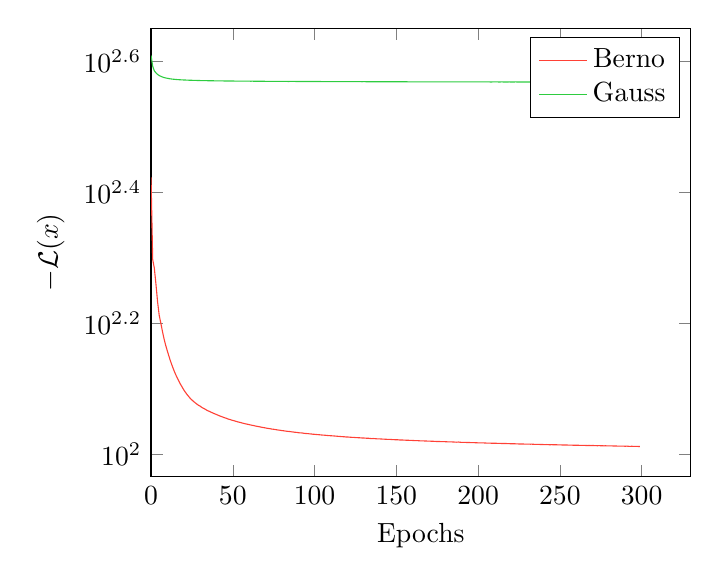
\begin{tikzpicture}\begin{semilogyaxis}    [% title={Comparison of Bernoulli and Gaussian},
    xlabel={Epochs},ylabel={$-\mathcal{L}(x)$},    xmin=0.0, xmax=330.0,ymin=92.5556732441, ymax=446.604102112,]    \addplot[color=red,]    coordinates {(0,264.441280629)(1,198.356619651)(2,192.436159585)(3,181.88292228)(4,170.867163613)(5,162.992125716)(6,158.524081254)(7,153.932894148)(8,149.911452137)(9,146.580097961)(10,143.728252064)(11,141.037141141)(12,138.570631631)(13,136.372970886)(14,134.325379597)(15,132.500336595)(16,130.871126321)(17,129.356009452)(18,127.971898707)(19,126.734941822)(20,125.497351657)(21,124.439595947)(22,123.45012017)(23,122.597523845)(24,121.760369304)(25,121.092850231)(26,120.448084176)(27,119.904902316)(28,119.36392291)(29,118.862854156)(30,118.50087892)(31,117.988382235)(32,117.637162698)(33,117.266831055)(34,116.858649569)(35,116.516663)(36,116.235720312)(37,115.906768508)(38,115.614068063)(39,115.31957292)(40,115.074554138)(41,114.762385753)(42,114.501882116)(43,114.261472196)(44,114.013497939)(45,113.760223153)(46,113.572592801)(47,113.29693616)(48,113.097699502)(49,112.896285359)(50,112.703451538)(51,112.534344316)(52,112.330035373)(53,112.128076033)(54,111.982370273)(55,111.833869726)(56,111.637882593)(57,111.479892134)(58,111.326744149)(59,111.203077074)(60,111.038512462)(61,110.916051622)(62,110.766563707)(63,110.65089404)(64,110.492657582)(65,110.373103416)(66,110.249482394)(67,110.115731964)(68,109.99644147)(69,109.878812866)(70,109.775324083)(71,109.634529669)(72,109.559145397)(73,109.445472745)(74,109.320581277)(75,109.244318709)(76,109.146542539)(77,109.045235651)(78,108.944406142)(79,108.870623821)(80,108.74620894)(81,108.68357537)(82,108.587148687)(83,108.508367004)(84,108.428299491)(85,108.377628465)(86,108.274904397)(87,108.215070093)(88,108.107207142)(89,108.082712153)(90,107.957791762)(91,107.885240506)(92,107.874081143)(93,107.774433053)(94,107.687143444)(95,107.63011365)(96,107.611140927)(97,107.495306466)(98,107.462627772)(99,107.365913835)(100,107.339672685)(101,107.266658963)(102,107.22216285)(103,107.166845037)(104,107.105922893)(105,107.046152371)(106,107.005534446)(107,106.951648865)(108,106.880565352)(109,106.854399705)(110,106.794855444)(111,106.763020269)(112,106.703687938)(113,106.668937961)(114,106.601654746)(115,106.561210799)(116,106.495546611)(117,106.447004936)(118,106.437038019)(119,106.348604292)(120,106.347453433)(121,106.292754641)(122,106.236165799)(123,106.202416687)(124,106.187918299)(125,106.117115784)(126,106.101480824)(127,106.043606304)(128,106.023886025)(129,105.969436354)(130,105.964091256)(131,105.911135712)(132,105.86270795)(133,105.870225164)(134,105.767693703)(135,105.744643374)(136,105.758845797)(137,105.714368258)(138,105.655033458)(139,105.641385567)(140,105.614113104)(141,105.581705725)(142,105.539112757)(143,105.510583621)(144,105.476887249)(145,105.440138453)(146,105.445337122)(147,105.399370769)(148,105.357715884)(149,105.329335896)(150,105.307112482)(151,105.289525036)(152,105.234197277)(153,105.229070324)(154,105.20831285)(155,105.151071847)(156,105.1411246)(157,105.129370228)(158,105.095529133)(159,105.084275596)(160,105.042046301)(161,105.009904993)(162,104.998100447)(163,104.974266926)(164,104.93239305)(165,104.892173295)(166,104.890742368)(167,104.868025471)(168,104.85551418)(169,104.81427887)(170,104.813642772)(171,104.77356111)(172,104.750256486)(173,104.733592613)(174,104.68709524)(175,104.667044109)(176,104.667854933)(177,104.634924524)(178,104.64095932)(179,104.608868741)(180,104.587649189)(181,104.556419886)(182,104.525155196)(183,104.513777729)(184,104.505319547)(185,104.481649905)(186,104.436392475)(187,104.407857527)(188,104.469331027)(189,104.376140886)(190,104.363132075)(191,104.363238498)(192,104.34758907)(193,104.30443383)(194,104.289089619)(195,104.282533639)(196,104.261895017)(197,104.250397228)(198,104.227165763)(199,104.207602178)(200,104.170897716)(201,104.174600997)(202,104.164283683)(203,104.150617357)(204,104.128893072)(205,104.092258578)(206,104.075724571)(207,104.087209722)(208,104.029951949)(209,104.036403101)(210,104.020640869)(211,104.009712275)(212,103.98694809)(213,103.983077642)(214,103.950611836)(215,103.933232394)(216,103.916490132)(217,103.929296903)(218,103.879854209)(219,103.88473698)(220,103.834719252)(221,103.859805159)(222,103.831793227)(223,103.818233573)(224,103.797998907)(225,103.757128629)(226,103.758065893)(227,103.759830114)(228,103.727329074)(229,103.707931477)(230,103.710236206)(231,103.704472323)(232,103.674412301)(233,103.683378046)(234,103.640059273)(235,103.602581829)(236,103.630522849)(237,103.601974529)(238,103.576733815)(239,103.578803697)(240,103.547068204)(241,103.532769429)(242,103.551075023)(243,103.51092109)(244,103.468415319)(245,103.506135961)(246,103.476072596)(247,103.482724679)(248,103.460180387)(249,103.446728724)(250,103.432438091)(251,103.409496515)(252,103.378862915)(253,103.401112227)(254,103.379215629)(255,103.360722476)(256,103.349105114)(257,103.3508815)(258,103.304165663)(259,103.310064087)(260,103.288380266)(261,103.291818959)(262,103.262840285)(263,103.266642706)(264,103.274717685)(265,103.241352428)(266,103.211669242)(267,103.179503618)(268,103.227792733)(269,103.176346006)(270,103.201589328)(271,103.179954973)(272,103.145690724)(273,103.125769265)(274,103.152660009)(275,103.1216678)(276,103.110800545)(277,103.083517359)(278,103.105228299)(279,103.071753457)(280,103.062483826)(281,103.064295557)(282,103.050972776)(283,103.019537784)(284,103.02247234)(285,103.00129278)(286,102.987354847)(287,102.988847032)(288,102.973827834)(289,102.970682553)(290,102.935659762)(291,102.965902446)(292,102.911485929)(293,102.906138472)(294,102.919145619)(295,102.90329698)(296,102.884802094)(297,102.887694439)(298,102.853640053)(299,102.839636938)    };    \addplot[color=green,]    coordinates {(0,406.003729193)(1,390.939739602)(2,384.54523432)(3,381.838768311)(4,379.759768122)(5,378.267186113)(6,377.267560591)(7,376.348206843)(8,375.579662365)(9,375.048516346)(10,374.609351751)(11,374.216701383)(12,373.866577259)(13,373.565440896)(14,373.319059115)(15,373.116086981)(16,372.93212308)(17,372.773892822)(18,372.669434482)(19,372.504596502)(20,372.41885498)(21,372.329580078)(22,372.231299383)(23,372.134079534)(24,372.090334861)(25,372.015324263)(26,371.884471047)(27,371.865363936)(28,371.796386774)(29,371.741563832)(30,371.674778109)(31,371.634727672)(32,371.582589)(33,371.502061768)(34,371.501245339)(35,371.444502064)(36,371.440941218)(37,371.371742665)(38,371.377627508)(39,371.31529025)(40,371.295935835)(41,371.26621177)(42,371.20323847)(43,371.202149492)(44,371.159871216)(45,371.140474243)(46,371.14647755)(47,371.070274991)(48,371.031648892)(49,371.081435991)(50,371.045891946)(51,371.002709628)(52,370.961609719)(53,370.946009244)(54,370.952441129)(55,370.911104237)(56,370.900569624)(57,370.877404119)(58,370.891667314)(59,370.853477173)(60,370.847278886)(61,370.829388317)(62,370.851452692)(63,370.779978305)(64,370.810793402)(65,370.767765669)(66,370.72699879)(67,370.736319136)(68,370.776238348)(69,370.716379228)(70,370.674620139)(71,370.676075661)(72,370.615640592)(73,370.648289906)(74,370.636204668)(75,370.601516335)(76,370.567452393)(77,370.606661488)(78,370.632338312)(79,370.568280862)(80,370.538198242)(81,370.483640414)(82,370.544183461)(83,370.544202104)(84,370.471667092)(85,370.509069769)(86,370.561665261)(87,370.513296009)(88,370.481637296)(89,370.444348921)(90,370.460461537)(91,370.443092762)(92,370.462338978)(93,370.429670077)(94,370.458904585)(95,370.454886697)(96,370.399512385)(97,370.422553655)(98,370.367223067)(99,370.358451483)(100,370.406783614)(101,370.340309948)(102,370.384053456)(103,370.434330389)(104,370.343586037)(105,370.327331931)(106,370.337170521)(107,370.3213395)(108,370.33544822)(109,370.287293868)(110,370.302190385)(111,370.2948392)(112,370.288230313)(113,370.252630893)(114,370.301730513)(115,370.235750732)(116,370.280508811)(117,370.257764116)(118,370.270446722)(119,370.209195168)(120,370.24347684)(121,370.227830644)(122,370.207783813)(123,370.195554754)(124,370.224240057)(125,370.217907826)(126,370.229621915)(127,370.194501454)(128,370.202709129)(129,370.179134577)(130,370.20087763)(131,370.174820279)(132,370.147938787)(133,370.134144897)(134,370.147430253)(135,370.145547763)(136,370.105337191)(137,370.161078769)(138,370.077486572)(139,370.16130532)(140,370.06839755)(141,370.124783325)(142,370.094960105)(143,370.139419445)(144,370.097701139)(145,370.100525901)(146,370.143301003)(147,370.105321655)(148,370.07771673)(149,370.137167414)(150,370.090415483)(151,370.101734675)(152,370.068199185)(153,370.083830733)(154,370.081583196)(155,370.086565996)(156,370.052335261)(157,370.02979753)(158,370.017346025)(159,370.037857999)(160,370.047184837)(161,370.014314908)(162,370.025267278)(163,370.021092585)(164,369.99633728)(165,369.986302157)(166,370.012848622)(167,369.971484375)(168,369.988048429)(169,369.98106523)(170,369.970600697)(171,369.977597268)(172,369.96486711)(173,369.993229093)(174,369.948671043)(175,369.978321866)(176,369.957537675)(177,369.98084345)(178,369.943227539)(179,369.921962502)(180,369.946230691)(181,369.976184637)(182,369.893339677)(183,369.976866233)(184,369.929182795)(185,369.950832575)(186,369.929775613)(187,369.937298251)(188,369.915333696)(189,369.905003995)(190,369.930191872)(191,369.942003063)(192,369.877530629)(193,369.930859042)(194,369.908915572)(195,369.902914151)(196,369.91256098)(197,369.88914806)(198,369.898595692)(199,369.880836293)(200,369.931452526)(201,369.897385365)(202,369.912643987)(203,369.864959384)(204,369.897603538)(205,369.906336226)(206,369.886783447)(207,369.86219488)(208,369.825184271)(209,369.908119285)(210,369.845081121)(211,369.849126199)(212,369.843999523)(213,369.831956399)(214,369.851669755)(215,369.861633079)(216,369.827253806)(217,369.835707397)(218,369.796921276)(219,369.847068481)(220,369.782892456)(221,369.82677862)(222,369.828237582)(223,369.866682351)(224,369.824126143)(225,369.81707464)(226,369.816195179)(227,369.826950795)(228,369.793815585)(229,369.792368663)(230,369.755177668)(231,369.803535156)(232,369.782006559)(233,369.755731922)(234,369.792746305)(235,369.763325528)(236,369.787186612)(237,369.740280429)(238,369.813177379)(239,369.771820457)(240,369.802965754)(241,369.749562711)(242,369.774524592)(243,369.746097745)(244,369.768768422)(245,369.815776367)(246,369.728163619)(247,369.754583019)(248,369.752389471)(249,369.748848211)(250,369.742936679)(251,369.74863481)(252,369.753147749)(253,369.751789495)(254,369.722884022)(255,369.767100664)(256,369.746748269)(257,369.736292114)(258,369.708355935)(259,369.72956776)(260,369.732071089)(261,369.705545821)(262,369.692340365)(263,369.71375061)(264,369.681090421)(265,369.704867942)(266,369.693760986)(267,369.71161954)(268,369.722984397)(269,369.741091253)(270,369.745334195)(271,369.704395807)(272,369.680385853)(273,369.675386242)(274,369.685295688)(275,369.674346203)(276,369.692077193)(277,369.719304643)(278,369.692321333)(279,369.655731479)(280,369.631802979)(281,369.686782227)(282,369.658116566)(283,369.656245228)(284,369.731848366)(285,369.705967463)(286,369.681227084)(287,369.659715854)(288,369.683410312)(289,369.651943248)(290,369.681238847)(291,369.654617587)(292,369.651562888)(293,369.653493486)(294,369.631222812)(295,369.661070113)(296,369.64445368)(297,369.702831643)(298,369.624187955)(299,369.650165905)    };    \legend{Berno,Gauss,}\end{semilogyaxis}\end{tikzpicture}\\}
  \caption{Bernoulli v.s Gaussian decoder distributions}
  \label{fig:bergau}
\end{wrapfigure}

\subsection{Importance Weighting}
In their 2015 publication \textit{Importance Weighted Autoencoders}, Burda, Grosse, and Salakhutdinov observed that Kingma \& Welling's $\L(x)$ lower bound on the log-likelihood from Eq.\ref{eq:VAEOBJECTIVE} made strong assumptions about the posterior inference, leading to overly simplified representations. They proposed an improvement called Importance Weighted Auto Encoders (IWAE), a generative model using the VAE network architecture with a few key improvements to model generalizability.
\par The critical feature of an IWAE is that the encoder network uses multiple importance weighted samples to approximate the posterior, where the original VAE uses a single sample. This allows IWAE to approximate complex posteriors which are not available under the stronger VAE posterior assumptions.
\par By considering multiple importance weighted samples we introduce a new lower bound on the log-likelihood which is strictly tighter than Eq.\ref{eq:VAEOBJECTIVE}.
\par Given $K$ independent samples $\{z_1,\mathellipsis,z_K\}$ from the encoder distribution $z_k\sim q_\phi(z|x)$ we define the new lower bound given by the $K$-sample importance weighting expectation of the log-likelihood:
\begin{equation}
   \L_K(x) = \mathbb{E}_{z_1,\mathellipsis,z_K \sim q_\phi(z|x)}\left[\log\frac{1}{K}\sum_{k=1}^{K}\frac{p_\theta(x,z_k)}{q_\phi(z_k|x)}\right]
\end{equation}
\begin{wrapfigure}{l}{0.5\textwidth}
  \captionsetup[subfigure]{justification=centering}
  \resizebox{\linewidth}{!}{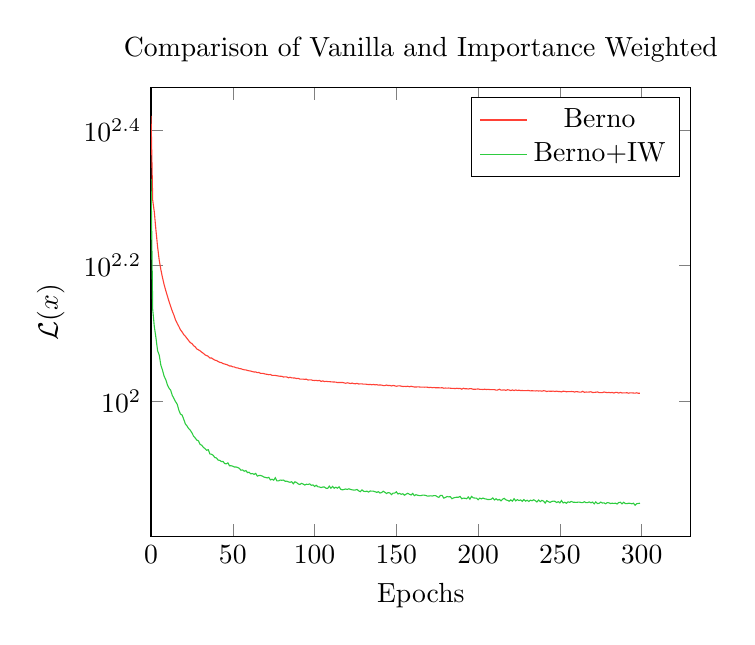
\begin{tikzpicture}\begin{semilogyaxis}    [title={Comparison of Vanilla and Importance Weighted},    xlabel={Epochs},ylabel={$\mathcal{L}(x)$},    xmin=0.0, xmax=330.0,ymin=63.1280970653, ymax=290.302163696,]    \addplot[color=red,]    coordinates {(0,263.911057906)(1,198.213255227)(2,190.304746094)(3,178.87626487)(4,169.086181335)(5,161.527062711)(6,156.384731972)(7,152.215601612)(8,148.611141996)(9,145.638506608)(10,142.924132968)(11,140.344120636)(12,137.979534649)(13,135.770691209)(14,133.905019739)(15,131.752419739)(16,130.218475314)(17,128.896445618)(18,127.414261669)(19,126.477938871)(20,125.370981806)(21,124.637320931)(22,123.725098253)(23,122.82003633)(24,121.97621564)(25,121.58177733)(26,120.742236287)(27,120.238140037)(28,119.374420554)(29,119.023158972)(30,118.607805509)(31,118.065131212)(32,117.60139052)(33,117.004031622)(34,116.718400712)(35,116.41280125)(36,115.757396102)(37,115.78068358)(38,115.311512451)(39,114.938878132)(40,114.766606986)(41,114.397145122)(42,114.068754716)(43,113.958563232)(44,113.586094263)(45,113.409035561)(46,113.245632921)(47,112.991837852)(48,112.665145236)(49,112.659438712)(50,112.346413921)(51,112.275464713)(52,111.965743034)(53,111.909392631)(54,111.668662997)(55,111.587927884)(56,111.359355261)(57,111.197885062)(58,111.16540107)(59,110.941213629)(60,110.819788527)(61,110.707621737)(62,110.529289024)(63,110.37031558)(64,110.406151165)(65,110.126960144)(66,110.205561454)(67,109.840602986)(68,109.876750807)(69,109.761879716)(70,109.585940247)(71,109.505338482)(72,109.363434989)(73,109.430629342)(74,109.109307736)(75,109.116950628)(76,109.086401492)(77,108.97200463)(78,108.851236808)(79,108.78205479)(80,108.765222321)(81,108.507579249)(82,108.57878135)(83,108.516908292)(84,108.210548054)(85,108.397520225)(86,108.204046173)(87,108.158662775)(88,108.119251099)(89,107.944731265)(90,108.016901661)(91,107.73954816)(92,107.710474063)(93,107.722989225)(94,107.645931951)(95,107.707727384)(96,107.39834155)(97,107.476644176)(98,107.438700867)(99,107.269752627)(100,107.226178214)(101,107.27347143)(102,107.135012554)(103,107.281838046)(104,106.898756478)(105,107.094956707)(106,106.842869887)(107,106.930941065)(108,106.833211892)(109,106.811454052)(110,106.74715787)(111,106.697943781)(112,106.671509316)(113,106.647949122)(114,106.467280981)(115,106.508278073)(116,106.494360435)(117,106.514126157)(118,106.379689359)(119,106.226369046)(120,106.389516629)(121,106.264832902)(122,106.141597665)(123,106.29064829)(124,106.089729767)(125,106.044406197)(126,106.192846985)(127,105.948057792)(128,106.009500122)(129,105.998451857)(130,105.889937189)(131,105.930427121)(132,105.831874473)(133,105.746641471)(134,105.81172312)(135,105.682832489)(136,105.784496613)(137,105.645301098)(138,105.740606662)(139,105.552423151)(140,105.615537886)(141,105.549215324)(142,105.395384771)(143,105.389573253)(144,105.572810267)(145,105.387793316)(146,105.453733201)(147,105.254012659)(148,105.439921903)(149,105.314982494)(150,105.142971275)(151,105.266738933)(152,105.306561043)(153,105.18495611)(154,105.064412842)(155,105.095941134)(156,105.06192129)(157,105.141722329)(158,104.962899822)(159,105.14358096)(160,104.997266513)(161,104.893339261)(162,104.877855197)(163,104.918052826)(164,104.899852669)(165,104.81209481)(166,104.848601851)(167,104.805977284)(168,104.821523576)(169,104.803668463)(170,104.667991735)(171,104.766617543)(172,104.629148407)(173,104.700370983)(174,104.605317577)(175,104.63054005)(176,104.611541415)(177,104.561938019)(178,104.629640406)(179,104.441594585)(180,104.512454348)(181,104.45640908)(182,104.514999376)(183,104.452973189)(184,104.380399669)(185,104.375079595)(186,104.317090399)(187,104.428788841)(188,104.330876146)(189,104.386269698)(190,104.100571511)(191,104.423475272)(192,104.240891294)(193,104.259876778)(194,104.166290921)(195,104.302629908)(196,104.255080955)(197,104.077226341)(198,104.0614371)(199,104.126844025)(200,104.175664645)(201,104.05645462)(202,104.047560023)(203,103.987927413)(204,104.079551905)(205,103.982308322)(206,104.042302163)(207,103.970290777)(208,103.958484331)(209,103.947987879)(210,103.96327172)(211,103.76637422)(212,103.808471305)(213,104.091310647)(214,103.776604892)(215,103.799186332)(216,103.860700254)(217,103.682867903)(218,103.907387848)(219,103.812983232)(220,103.614567913)(221,103.836631248)(222,103.59787495)(223,103.838682875)(224,103.65001125)(225,103.76185207)(226,103.608184717)(227,103.631562625)(228,103.600637956)(229,103.59588716)(230,103.617301331)(231,103.645032404)(232,103.505390778)(233,103.568912243)(234,103.512093561)(235,103.475622905)(236,103.542617298)(237,103.458997664)(238,103.525815666)(239,103.391191656)(240,103.57085022)(241,103.501735021)(242,103.269330347)(243,103.432664781)(244,103.366980355)(245,103.361040011)(246,103.434469188)(247,103.279656011)(248,103.424536896)(249,103.280434931)(250,103.293235501)(251,103.138385315)(252,103.381104029)(253,103.340434723)(254,103.193569599)(255,103.243596954)(256,103.220414692)(257,103.283062328)(258,103.251557936)(259,103.102934931)(260,103.248284232)(261,103.181984031)(262,103.060927512)(263,103.05878762)(264,103.356516363)(265,102.997390858)(266,103.102375141)(267,103.061714866)(268,103.104844236)(269,103.193875705)(270,102.934247242)(271,102.966972268)(272,103.023014429)(273,103.135971902)(274,102.914399802)(275,102.884195876)(276,102.911637296)(277,103.110926569)(278,102.980401265)(279,102.88293611)(280,102.968769601)(281,102.855491666)(282,102.971831748)(283,102.752470301)(284,102.950700476)(285,102.961044977)(286,102.733744424)(287,102.971840598)(288,102.765343822)(289,102.825684038)(290,102.796692491)(291,102.862699835)(292,102.688350164)(293,102.817591525)(294,102.802225425)(295,102.750529341)(296,102.698477298)(297,102.824272738)(298,102.667397516)(299,102.672452365)    };    \addplot[color=green,]    coordinates {(0,212.889503881)(1,136.69067473)(2,128.82833134)(3,124.040854936)(4,118.690849804)(5,116.909000924)(6,113.013927626)(7,111.075254586)(8,108.798369917)(9,107.562806091)(10,105.667284851)(11,104.449745872)(12,103.738867798)(13,101.913222407)(14,100.880470165)(15,99.7707582092)(16,98.9113952359)(17,96.9467745001)(18,95.6420740024)(19,95.3488831676)(20,93.9665334251)(21,92.4877756431)(22,91.8431637018)(23,91.0363048068)(24,90.5232136397)(25,89.7399208069)(26,88.7281854803)(27,88.1798480225)(28,87.5367355208)(29,87.3209809875)(30,86.2576438349)(31,86.0276815102)(32,85.4221434021)(33,85.0303677923)(34,84.5800309337)(35,84.7152453891)(36,83.5131790022)(37,83.4104959453)(38,83.1304513758)(39,82.4841615989)(40,82.3764996546)(41,81.7875932936)(42,81.7060721588)(43,81.3806930681)(44,81.4111268546)(45,80.838586731)(46,80.7406091725)(47,81.017188041)(48,80.2124638228)(49,80.2271451361)(50,80.0896083138)(51,79.8871128637)(52,79.8942684867)(53,79.7550364408)(54,79.538298645)(55,79.0118305414)(56,79.0969413133)(57,78.7534699735)(58,78.9117192979)(59,78.3776827171)(60,78.4891304779)(61,78.0464635398)(62,78.1325949721)(63,77.9003106967)(64,78.1739014712)(65,77.4500395133)(66,77.6281871865)(67,77.6110464131)(68,77.474847426)(69,77.2124328683)(70,77.1030504678)(71,76.9742827121)(72,77.1269824912)(73,76.453514002)(74,76.6268032559)(75,76.3920169484)(76,77.0279490245)(77,76.1911592518)(78,76.1912690319)(79,76.4120253546)(80,76.3616653512)(81,76.4200014773)(82,76.1013489741)(83,76.1299544941)(84,75.9456712133)(85,75.8474544456)(86,75.9958151453)(87,75.4516047114)(88,75.9606080211)(89,75.7825870514)(90,75.4166851807)(91,75.2730201028)(92,75.5633785178)(93,75.3926641221)(94,75.1231771504)(95,75.3425059509)(96,75.2793357017)(97,75.42107236)(98,75.0752778209)(99,75.1563735268)(100,74.7741940308)(101,75.0860549094)(102,74.687021852)(103,74.6451232633)(104,74.4814327032)(105,74.6204650948)(106,74.6206243688)(107,74.3239216544)(108,74.2764617642)(109,74.8516898277)(110,74.3182112052)(111,74.7670684121)(112,74.3290488018)(113,74.5695130088)(114,74.3323224362)(115,74.6895237246)(116,74.0510518993)(117,73.9067425815)(118,74.0074700442)(119,74.1338988495)(120,74.0175181926)(121,74.1761847895)(122,74.0235229562)(123,73.9181140345)(124,73.8457655473)(125,73.8702288749)(126,74.0162856362)(127,73.6437659316)(128,73.4565949943)(129,73.9170945116)(130,73.5467081313)(131,73.4937463864)(132,73.5905630146)(133,73.353295621)(134,73.6264864766)(135,73.5908654092)(136,73.5732003923)(137,73.4532649994)(138,73.2716727794)(139,73.465524188)(140,73.112097598)(141,73.2420930204)(142,73.5635126287)(143,73.3090762398)(144,72.9897125105)(145,73.2172430489)(146,73.1516952931)(147,72.7228497869)(148,73.0782187098)(149,73.1016768508)(150,73.4024589885)(151,72.880766879)(152,73.0312317588)(153,72.7873863844)(154,72.9423721105)(155,72.5628787509)(156,72.8360966284)(157,73.047174426)(158,72.8167339325)(159,72.6396780465)(160,73.0304298262)(161,72.4665298601)(162,72.6912430434)(163,72.5760772358)(164,72.4846100339)(165,72.459022411)(166,72.5838312045)(167,72.6003749293)(168,72.5145784413)(169,72.3569016474)(170,72.3737294076)(171,72.4213695249)(172,72.3710491943)(173,72.4755430534)(174,72.4657969249)(175,72.2095316592)(176,72.0375349288)(177,72.5440174311)(178,72.5334384502)(179,71.8655854936)(180,72.008425508)(181,72.254446425)(182,72.1637018724)(183,72.2237791096)(184,71.714810257)(185,71.9142984702)(186,72.0176052856)(187,72.0815261771)(188,72.0838776606)(189,72.2727386128)(190,71.688610285)(191,71.8585383883)(192,71.8177259757)(193,71.7062380357)(194,72.1454219471)(195,71.6026708776)(196,72.2864398055)(197,71.9247254597)(198,71.868394928)(199,71.8450078375)(200,71.4535544239)(201,71.8534567261)(202,71.670494683)(203,71.8755769626)(204,71.7016650391)(205,71.6363452565)(206,71.504623205)(207,71.5315711698)(208,71.587473741)(209,71.8978508828)(210,71.4103687564)(211,71.70563883)(212,71.3756308677)(213,71.5474994174)(214,71.1844528337)(215,71.60504733)(216,71.8060398934)(217,71.4310690862)(218,71.3169561282)(219,71.1020025912)(220,71.425415476)(221,71.1148356559)(222,71.7071190435)(223,71.1754220234)(224,71.483830067)(225,71.261985321)(226,71.4267416937)(227,71.0780576116)(228,71.5027765656)(229,71.1248665203)(230,71.3434074541)(231,71.0519401204)(232,71.3568696039)(233,71.2187969555)(234,71.4516134782)(235,71.2335008032)(236,70.9221232674)(237,71.3969466123)(238,70.9965213568)(239,71.3100876895)(240,71.1295058164)(241,70.6539552723)(242,71.2394960577)(243,70.9955520907)(244,70.8132880679)(245,71.0490945296)(246,71.1247871052)(247,71.0870736417)(248,70.7841236739)(249,70.9903914504)(250,70.7095126967)(251,71.2655674189)(252,70.6899923706)(253,70.8693695623)(254,70.6116099063)(255,70.951697138)(256,70.8354414368)(257,71.0545902252)(258,70.8714400898)(259,70.8538174022)(260,70.822078039)(261,70.8707302163)(262,70.8950232905)(263,70.7760084395)(264,70.7706362083)(265,70.9704128127)(266,70.7572787822)(267,70.7819294947)(268,70.9383078766)(269,70.7281015916)(270,70.8945835599)(271,70.482622972)(272,70.93528905)(273,70.5277008334)(274,70.5941716211)(275,70.8907409599)(276,70.6606239388)(277,70.7143197632)(278,70.4889673545)(279,70.7734613106)(280,70.716083048)(281,70.5357097002)(282,70.6280721283)(283,70.5701076577)(284,70.6263676938)(285,70.4352469635)(286,70.7839288816)(287,70.8557285656)(288,70.4485128229)(289,70.8420001637)(290,70.5595037981)(291,70.5228122572)(292,70.6055964106)(293,70.5968888716)(294,70.4848312725)(295,70.6190093855)(296,70.1423300726)(297,70.5032779763)(298,70.5609679066)(299,70.6179385029)    };    \legend{Berno,Berno+IW,}\end{semilogyaxis}\end{tikzpicture}\\}
  \caption{Variational v.s. Importance Weighted (IW)}
  \label{fig:variw}
\end{wrapfigure}
The term inside the sum is the normalized importance weights for the joint distribution. Note in particular that the case $K=1$ corresponds exactly to Kingma \& Welling's $\L(x)$ from Eq.\ref{eq:VAEOBJECTIVE}. Burda, Grosse, and Salakhutdinov show that this importance weighted lower bound is strictly tighter than the vanilla lower bound. In particular, that $\log p(x) \geq \L_{K+1}(x)>\L_K(x)$ Our implementation of IWAE with this lower bound supports their findings. We observed that with $K=5$ samples IWAE significantly improves the learned log-likelihood bound during training. The results of this experiment can be found in Figure \ref{fig:variw}. Since importance weighting so significantly improved the performance of our Auto Encoder, all further methods were implemented on VAEs with importance weighting.
\subsection{Batch Normalization}
Batch normalization is a recent method developed to improve stability and convergence speed in deep networks \cite{Ioffe2015}. In the recent paper \textit{How to Train Deep Variational Autoencoders and Probabilistic Ladder Networks} by S\o nderby et al. 2016, the authors show that batch normalization is an important method for learning deep VAEs \cite{Sonderby2016}. That is, deep generative models with several latent layers. Though we are only considering a shallow model with a single latent layer, we were interested to see how batch normalization affected training as well as latent space activity (discussed in later sections).
\begin{wrapfigure}{l}{0.5\textwidth}
    \resizebox{\linewidth}{!}{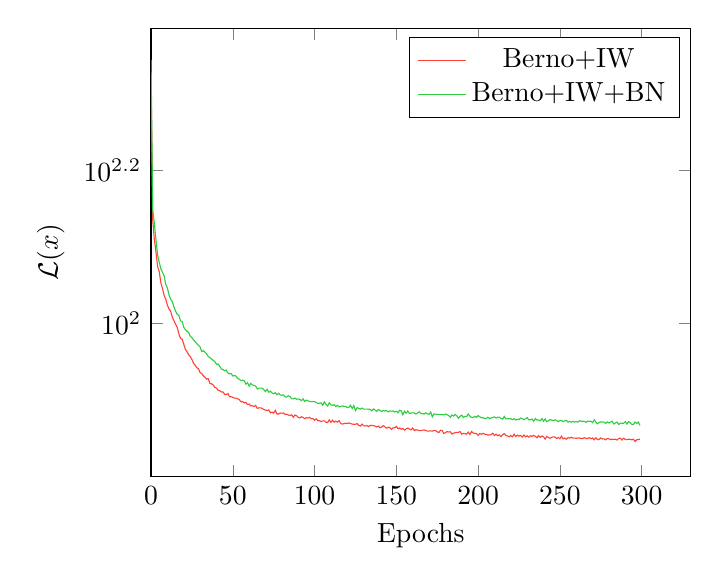
\begin{tikzpicture}\begin{semilogyaxis}    [% title={Comparison of Importance Weighted and Batch Normalized},
    xlabel={Epochs},ylabel={$\mathcal{L}(x)$},    xmin=0.0, xmax=330.0,ymin=63.1280970653, ymax=242.893315674,]    \addplot[color=red,]    coordinates {(0,212.889503881)(1,136.69067473)(2,128.82833134)(3,124.040854936)(4,118.690849804)(5,116.909000924)(6,113.013927626)(7,111.075254586)(8,108.798369917)(9,107.562806091)(10,105.667284851)(11,104.449745872)(12,103.738867798)(13,101.913222407)(14,100.880470165)(15,99.7707582092)(16,98.9113952359)(17,96.9467745001)(18,95.6420740024)(19,95.3488831676)(20,93.9665334251)(21,92.4877756431)(22,91.8431637018)(23,91.0363048068)(24,90.5232136397)(25,89.7399208069)(26,88.7281854803)(27,88.1798480225)(28,87.5367355208)(29,87.3209809875)(30,86.2576438349)(31,86.0276815102)(32,85.4221434021)(33,85.0303677923)(34,84.5800309337)(35,84.7152453891)(36,83.5131790022)(37,83.4104959453)(38,83.1304513758)(39,82.4841615989)(40,82.3764996546)(41,81.7875932936)(42,81.7060721588)(43,81.3806930681)(44,81.4111268546)(45,80.838586731)(46,80.7406091725)(47,81.017188041)(48,80.2124638228)(49,80.2271451361)(50,80.0896083138)(51,79.8871128637)(52,79.8942684867)(53,79.7550364408)(54,79.538298645)(55,79.0118305414)(56,79.0969413133)(57,78.7534699735)(58,78.9117192979)(59,78.3776827171)(60,78.4891304779)(61,78.0464635398)(62,78.1325949721)(63,77.9003106967)(64,78.1739014712)(65,77.4500395133)(66,77.6281871865)(67,77.6110464131)(68,77.474847426)(69,77.2124328683)(70,77.1030504678)(71,76.9742827121)(72,77.1269824912)(73,76.453514002)(74,76.6268032559)(75,76.3920169484)(76,77.0279490245)(77,76.1911592518)(78,76.1912690319)(79,76.4120253546)(80,76.3616653512)(81,76.4200014773)(82,76.1013489741)(83,76.1299544941)(84,75.9456712133)(85,75.8474544456)(86,75.9958151453)(87,75.4516047114)(88,75.9606080211)(89,75.7825870514)(90,75.4166851807)(91,75.2730201028)(92,75.5633785178)(93,75.3926641221)(94,75.1231771504)(95,75.3425059509)(96,75.2793357017)(97,75.42107236)(98,75.0752778209)(99,75.1563735268)(100,74.7741940308)(101,75.0860549094)(102,74.687021852)(103,74.6451232633)(104,74.4814327032)(105,74.6204650948)(106,74.6206243688)(107,74.3239216544)(108,74.2764617642)(109,74.8516898277)(110,74.3182112052)(111,74.7670684121)(112,74.3290488018)(113,74.5695130088)(114,74.3323224362)(115,74.6895237246)(116,74.0510518993)(117,73.9067425815)(118,74.0074700442)(119,74.1338988495)(120,74.0175181926)(121,74.1761847895)(122,74.0235229562)(123,73.9181140345)(124,73.8457655473)(125,73.8702288749)(126,74.0162856362)(127,73.6437659316)(128,73.4565949943)(129,73.9170945116)(130,73.5467081313)(131,73.4937463864)(132,73.5905630146)(133,73.353295621)(134,73.6264864766)(135,73.5908654092)(136,73.5732003923)(137,73.4532649994)(138,73.2716727794)(139,73.465524188)(140,73.112097598)(141,73.2420930204)(142,73.5635126287)(143,73.3090762398)(144,72.9897125105)(145,73.2172430489)(146,73.1516952931)(147,72.7228497869)(148,73.0782187098)(149,73.1016768508)(150,73.4024589885)(151,72.880766879)(152,73.0312317588)(153,72.7873863844)(154,72.9423721105)(155,72.5628787509)(156,72.8360966284)(157,73.047174426)(158,72.8167339325)(159,72.6396780465)(160,73.0304298262)(161,72.4665298601)(162,72.6912430434)(163,72.5760772358)(164,72.4846100339)(165,72.459022411)(166,72.5838312045)(167,72.6003749293)(168,72.5145784413)(169,72.3569016474)(170,72.3737294076)(171,72.4213695249)(172,72.3710491943)(173,72.4755430534)(174,72.4657969249)(175,72.2095316592)(176,72.0375349288)(177,72.5440174311)(178,72.5334384502)(179,71.8655854936)(180,72.008425508)(181,72.254446425)(182,72.1637018724)(183,72.2237791096)(184,71.714810257)(185,71.9142984702)(186,72.0176052856)(187,72.0815261771)(188,72.0838776606)(189,72.2727386128)(190,71.688610285)(191,71.8585383883)(192,71.8177259757)(193,71.7062380357)(194,72.1454219471)(195,71.6026708776)(196,72.2864398055)(197,71.9247254597)(198,71.868394928)(199,71.8450078375)(200,71.4535544239)(201,71.8534567261)(202,71.670494683)(203,71.8755769626)(204,71.7016650391)(205,71.6363452565)(206,71.504623205)(207,71.5315711698)(208,71.587473741)(209,71.8978508828)(210,71.4103687564)(211,71.70563883)(212,71.3756308677)(213,71.5474994174)(214,71.1844528337)(215,71.60504733)(216,71.8060398934)(217,71.4310690862)(218,71.3169561282)(219,71.1020025912)(220,71.425415476)(221,71.1148356559)(222,71.7071190435)(223,71.1754220234)(224,71.483830067)(225,71.261985321)(226,71.4267416937)(227,71.0780576116)(228,71.5027765656)(229,71.1248665203)(230,71.3434074541)(231,71.0519401204)(232,71.3568696039)(233,71.2187969555)(234,71.4516134782)(235,71.2335008032)(236,70.9221232674)(237,71.3969466123)(238,70.9965213568)(239,71.3100876895)(240,71.1295058164)(241,70.6539552723)(242,71.2394960577)(243,70.9955520907)(244,70.8132880679)(245,71.0490945296)(246,71.1247871052)(247,71.0870736417)(248,70.7841236739)(249,70.9903914504)(250,70.7095126967)(251,71.2655674189)(252,70.6899923706)(253,70.8693695623)(254,70.6116099063)(255,70.951697138)(256,70.8354414368)(257,71.0545902252)(258,70.8714400898)(259,70.8538174022)(260,70.822078039)(261,70.8707302163)(262,70.8950232905)(263,70.7760084395)(264,70.7706362083)(265,70.9704128127)(266,70.7572787822)(267,70.7819294947)(268,70.9383078766)(269,70.7281015916)(270,70.8945835599)(271,70.482622972)(272,70.93528905)(273,70.5277008334)(274,70.5941716211)(275,70.8907409599)(276,70.6606239388)(277,70.7143197632)(278,70.4889673545)(279,70.7734613106)(280,70.716083048)(281,70.5357097002)(282,70.6280721283)(283,70.5701076577)(284,70.6263676938)(285,70.4352469635)(286,70.7839288816)(287,70.8557285656)(288,70.4485128229)(289,70.8420001637)(290,70.5595037981)(291,70.5228122572)(292,70.6055964106)(293,70.5968888716)(294,70.4848312725)(295,70.6190093855)(296,70.1423300726)(297,70.5032779763)(298,70.5609679066)(299,70.6179385029)    };    \addplot[color=green,]    coordinates {(0,220.812105158)(1,140.868051827)(2,135.319417752)(3,128.724276525)(4,122.955164934)(5,120.300830952)(6,117.842742795)(7,116.64050999)(8,115.456067366)(9,112.34451896)(10,111.265299988)(11,108.952617645)(12,107.563851083)(13,106.774169367)(14,105.103744632)(15,103.802531835)(16,102.803668574)(17,102.481998249)(18,100.802762729)(19,100.585010515)(20,98.9090365462)(21,98.1169030346)(22,97.765475991)(23,97.2764186928)(24,96.245937181)(25,95.8124569841)(26,95.1456111839)(27,94.6529702898)(28,94.1195864868)(29,93.6386244618)(30,93.1986750516)(31,91.8884819724)(32,92.1219651656)(33,91.7660386519)(34,91.250533586)(35,90.5151538641)(36,90.2425081288)(37,89.9071646812)(38,89.4961200783)(39,89.1786010881)(40,88.4559831515)(41,88.51847229)(42,87.9428533242)(43,87.1944852101)(44,87.0648347751)(45,86.7229512579)(46,86.9227582203)(47,86.1712326466)(48,85.950587068)(49,86.04926608)(50,85.3923743786)(51,85.5322129267)(52,85.3271336781)(53,84.8019374084)(54,84.536986951)(55,84.2305892389)(56,84.3286683377)(57,84.1522436732)(58,83.3012238104)(59,83.7155057456)(60,82.7992233693)(61,83.5205334057)(62,83.1124755651)(63,83.0196700356)(64,82.8275105979)(65,82.1291870949)(66,82.3226089686)(67,82.3403921648)(68,82.3120443171)(69,81.9174896448)(70,81.5030302568)(71,82.0591559809)(72,81.3132039018)(73,81.591406354)(74,81.1437691914)(75,80.9562143222)(76,81.1953004109)(77,80.6989246923)(78,81.0439923997)(79,80.7104799097)(80,80.579273647)(81,80.6894023687)(82,80.1604832944)(83,80.1868576397)(84,80.4712490706)(85,80.2842603579)(86,79.7442494479)(87,79.7343605735)(88,79.9086901647)(89,79.635063428)(90,79.741575685)(91,79.5902122983)(92,79.2991520483)(93,79.7187010609)(94,79.1092982483)(95,79.4226407693)(96,79.2733724282)(97,79.1051692338)(98,79.0754059809)(99,79.1018828097)(100,79.0593816376)(101,78.9150700933)(102,78.6440699699)(103,78.6818985402)(104,78.7929203033)(105,78.1865223347)(106,79.0145359802)(107,78.4409182462)(108,78.0524690108)(109,78.8077469358)(110,78.2960041046)(111,78.1936078644)(112,78.3528583457)(113,77.9041483238)(114,78.1752235205)(115,77.8163253368)(116,77.9147369385)(117,78.0464619376)(118,77.9532819644)(119,77.9274888819)(120,77.6990697479)(121,77.7212414135)(122,78.2119804313)(123,77.451852091)(124,78.1315626803)(125,76.9649418432)(126,77.6510731576)(127,77.4836851571)(128,77.3073894709)(129,77.5475659943)(130,77.2900101055)(131,77.294678206)(132,77.3047630587)(133,77.2909118236)(134,77.2878407634)(135,76.902970907)(136,77.3512902208)(137,77.1018692849)(138,76.7875662162)(139,77.2080883581)(140,77.0465301098)(141,76.7734781647)(142,76.9981128554)(143,76.8602037048)(144,77.0179359089)(145,76.6783211795)(146,76.887396268)(147,76.8487717438)(148,76.8828933646)(149,76.647767112)(150,76.8185476893)(151,76.4525053753)(152,77.0563210227)(153,76.8780969932)(154,75.9855017992)(155,76.8270853493)(156,76.3929172169)(157,76.8689556191)(158,76.309076219)(159,76.3741976166)(160,76.4659639948)(161,76.4167646165)(162,76.1588406788)(163,76.3985902058)(164,76.6891410065)(165,76.2885811199)(166,76.2813544395)(167,76.1354372267)(168,76.4683616222)(169,76.2195049425)(170,76.0912478707)(171,76.6379284737)(172,75.5368430675)(173,76.2009703549)(174,76.1571691686)(175,76.094223286)(176,76.0969603105)(177,76.0537287279)(178,76.031106505)(179,75.9697008722)(180,76.1766836964)(181,76.0215624861)(182,75.862494486)(183,75.431596867)(184,75.9766488231)(185,75.7119712067)(186,76.0821262498)(187,75.7707103799)(188,75.1897688363)(189,75.6704169533)(190,75.9127686449)(191,75.4278393763)(192,75.6543837253)(193,75.6135286505)(194,76.2010392206)(195,75.6841124101)(196,75.3987940424)(197,75.3748238234)(198,75.6606351887)(199,75.4237091203)(200,75.814623961)(201,75.5699364263)(202,75.2985267292)(203,75.3570597284)(204,75.1684181213)(205,75.1631805767)(206,75.4559900457)(207,75.1224482172)(208,75.3214972063)(209,75.3767447038)(210,75.5251281738)(211,75.2924619501)(212,75.4850157166)(213,75.4524022883)(214,75.191533869)(215,75.0114420249)(216,75.6158445601)(217,75.0702012426)(218,75.0961439167)(219,75.124752121)(220,75.1005330519)(221,74.893462566)(222,75.1368557531)(223,74.8167615856)(224,74.9818515986)(225,74.9404246035)(226,75.2453195329)(227,75.1283115734)(228,74.9109797738)(229,75.103415777)(230,75.3592353058)(231,74.8492726482)(232,74.8929144565)(233,75.032299118)(234,74.5508918693)(235,75.1469980205)(236,74.8126035794)(237,74.8305967782)(238,74.6399993966)(239,75.1417248535)(240,74.556847874)(241,75.0714584628)(242,74.4212250103)(243,74.6612699266)(244,74.9332658733)(245,74.7995458221)(246,74.6834466622)(247,74.8652081229)(248,74.724238524)(249,74.4261099451)(250,74.7198648904)(251,74.7438465743)(252,74.4551574222)(253,74.6536740459)(254,74.7526102794)(255,74.3327881414)(256,74.5383223516)(257,74.3206366036)(258,74.522478603)(259,74.3381154216)(260,74.4665795552)(261,74.3358595623)(262,74.6770175864)(263,74.5301153842)(264,74.5491240345)(265,74.5142330655)(266,74.2829835094)(267,74.5868861389)(268,74.5018216705)(269,74.5457204853)(270,74.2275134763)(271,74.8797874797)(272,74.3535444294)(273,73.9741289312)(274,74.2580836209)(275,74.3988033711)(276,74.3752106198)(277,74.3335512335)(278,74.0707263738)(279,74.4006223158)(280,74.1427292494)(281,74.3383737044)(282,74.5402551686)(283,73.9278499881)(284,74.1787790402)(285,74.3597446858)(286,73.8246305778)(287,74.1425923504)(288,74.0815582622)(289,74.0791946827)(290,74.4631946841)(291,73.9177805467)(292,74.4376518111)(293,74.2326508817)(294,73.8226823009)(295,73.8183200836)(296,74.3854140889)(297,74.0012052363)(298,74.3635426539)(299,73.5976050429)    };    \legend{Berno+IW,Berno+IW+BN,}\end{semilogyaxis}\end{tikzpicture}\\}
    \caption{Effect of Batch Normalization (BN)}
    \label{fig:bncost}
\end{wrapfigure}
\par Batch normalization was developed to improve learning stability during deep network training. As parameters change during learning the layer output distributions change for each hidden layer, requiring later layers to adjust parameters in response to these distribution changes. The problem that batch normalization attempts to address is that changes in early layer output distributions can cause noisy changes to later layers. 
\par Batch normalization functions by normalizing the inputs of the activation function for each layer so that the inputs across each training batch have a mean of 0 and a variance of 1. However, batch normalization restricts the representation of each layer by assuming this normal distribution. To alleviate some of this restriction, batch normalization introduces learnable parameters to scale the variance of the normal distribution, $\gamma$ and shift the mean, $\beta$. Therefore, we transform each activation function input, $x_i$, with the batch normalization given by:

\begin{align*}
    \text{BN}(x_i)=\gamma\left(\frac{x_i-\mu_B}{\sqrt{\sigma_B^2+\epsilon}}\right)+\beta\\
\end{align*} 
where $\mu_B$ and $\sigma_B$ are the mean and standard deviation of the layer's activation function input across the batch, $\epsilon$ is a small constant addition to the variance to avoid division by 0, and $\gamma$ and $\beta$ are learnable scale and shift parameters. Note in particular that when learning with batch normalization, the learned shift parameter $\beta$ for each layer replaces the need for bias terms added to that layer's activation inputs.
\begin{wrapfigure}{l}{0.5\textwidth}
    \resizebox{\linewidth}{!}{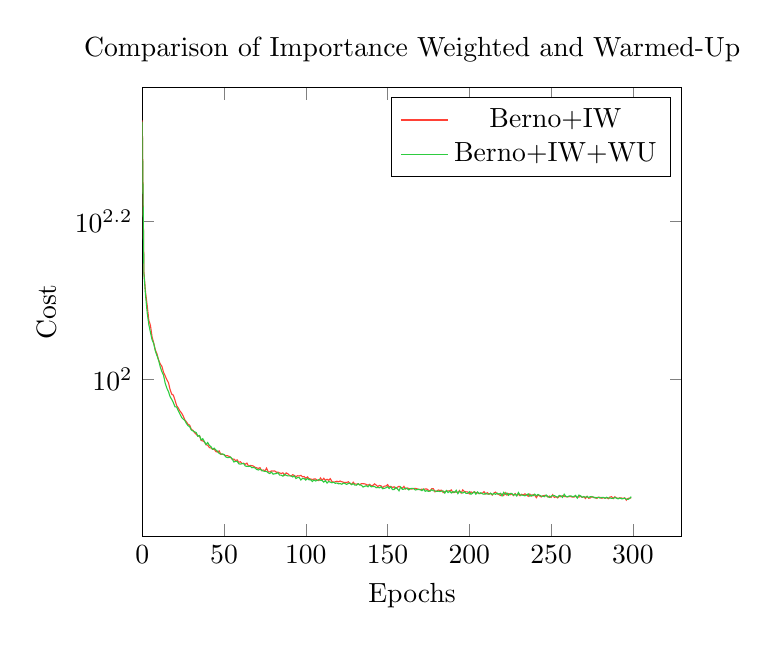
\begin{tikzpicture}\begin{semilogyaxis}    [title={Comparison of Importance Weighted and Warmed-Up},    xlabel={Epochs},ylabel={Cost},    xmin=0.0, xmax=330.0,ymin=63.1280970653, ymax=234.178454269,]    \addplot[color=red,]    coordinates {(0,212.889503881)(1,136.69067473)(2,128.82833134)(3,124.040854936)(4,118.690849804)(5,116.909000924)(6,113.013927626)(7,111.075254586)(8,108.798369917)(9,107.562806091)(10,105.667284851)(11,104.449745872)(12,103.738867798)(13,101.913222407)(14,100.880470165)(15,99.7707582092)(16,98.9113952359)(17,96.9467745001)(18,95.6420740024)(19,95.3488831676)(20,93.9665334251)(21,92.4877756431)(22,91.8431637018)(23,91.0363048068)(24,90.5232136397)(25,89.7399208069)(26,88.7281854803)(27,88.1798480225)(28,87.5367355208)(29,87.3209809875)(30,86.2576438349)(31,86.0276815102)(32,85.4221434021)(33,85.0303677923)(34,84.5800309337)(35,84.7152453891)(36,83.5131790022)(37,83.4104959453)(38,83.1304513758)(39,82.4841615989)(40,82.3764996546)(41,81.7875932936)(42,81.7060721588)(43,81.3806930681)(44,81.4111268546)(45,80.838586731)(46,80.7406091725)(47,81.017188041)(48,80.2124638228)(49,80.2271451361)(50,80.0896083138)(51,79.8871128637)(52,79.8942684867)(53,79.7550364408)(54,79.538298645)(55,79.0118305414)(56,79.0969413133)(57,78.7534699735)(58,78.9117192979)(59,78.3776827171)(60,78.4891304779)(61,78.0464635398)(62,78.1325949721)(63,77.9003106967)(64,78.1739014712)(65,77.4500395133)(66,77.6281871865)(67,77.6110464131)(68,77.474847426)(69,77.2124328683)(70,77.1030504678)(71,76.9742827121)(72,77.1269824912)(73,76.453514002)(74,76.6268032559)(75,76.3920169484)(76,77.0279490245)(77,76.1911592518)(78,76.1912690319)(79,76.4120253546)(80,76.3616653512)(81,76.4200014773)(82,76.1013489741)(83,76.1299544941)(84,75.9456712133)(85,75.8474544456)(86,75.9958151453)(87,75.4516047114)(88,75.9606080211)(89,75.7825870514)(90,75.4166851807)(91,75.2730201028)(92,75.5633785178)(93,75.3926641221)(94,75.1231771504)(95,75.3425059509)(96,75.2793357017)(97,75.42107236)(98,75.0752778209)(99,75.1563735268)(100,74.7741940308)(101,75.0860549094)(102,74.687021852)(103,74.6451232633)(104,74.4814327032)(105,74.6204650948)(106,74.6206243688)(107,74.3239216544)(108,74.2764617642)(109,74.8516898277)(110,74.3182112052)(111,74.7670684121)(112,74.3290488018)(113,74.5695130088)(114,74.3323224362)(115,74.6895237246)(116,74.0510518993)(117,73.9067425815)(118,74.0074700442)(119,74.1338988495)(120,74.0175181926)(121,74.1761847895)(122,74.0235229562)(123,73.9181140345)(124,73.8457655473)(125,73.8702288749)(126,74.0162856362)(127,73.6437659316)(128,73.4565949943)(129,73.9170945116)(130,73.5467081313)(131,73.4937463864)(132,73.5905630146)(133,73.353295621)(134,73.6264864766)(135,73.5908654092)(136,73.5732003923)(137,73.4532649994)(138,73.2716727794)(139,73.465524188)(140,73.112097598)(141,73.2420930204)(142,73.5635126287)(143,73.3090762398)(144,72.9897125105)(145,73.2172430489)(146,73.1516952931)(147,72.7228497869)(148,73.0782187098)(149,73.1016768508)(150,73.4024589885)(151,72.880766879)(152,73.0312317588)(153,72.7873863844)(154,72.9423721105)(155,72.5628787509)(156,72.8360966284)(157,73.047174426)(158,72.8167339325)(159,72.6396780465)(160,73.0304298262)(161,72.4665298601)(162,72.6912430434)(163,72.5760772358)(164,72.4846100339)(165,72.459022411)(166,72.5838312045)(167,72.6003749293)(168,72.5145784413)(169,72.3569016474)(170,72.3737294076)(171,72.4213695249)(172,72.3710491943)(173,72.4755430534)(174,72.4657969249)(175,72.2095316592)(176,72.0375349288)(177,72.5440174311)(178,72.5334384502)(179,71.8655854936)(180,72.008425508)(181,72.254446425)(182,72.1637018724)(183,72.2237791096)(184,71.714810257)(185,71.9142984702)(186,72.0176052856)(187,72.0815261771)(188,72.0838776606)(189,72.2727386128)(190,71.688610285)(191,71.8585383883)(192,71.8177259757)(193,71.7062380357)(194,72.1454219471)(195,71.6026708776)(196,72.2864398055)(197,71.9247254597)(198,71.868394928)(199,71.8450078375)(200,71.4535544239)(201,71.8534567261)(202,71.670494683)(203,71.8755769626)(204,71.7016650391)(205,71.6363452565)(206,71.504623205)(207,71.5315711698)(208,71.587473741)(209,71.8978508828)(210,71.4103687564)(211,71.70563883)(212,71.3756308677)(213,71.5474994174)(214,71.1844528337)(215,71.60504733)(216,71.8060398934)(217,71.4310690862)(218,71.3169561282)(219,71.1020025912)(220,71.425415476)(221,71.1148356559)(222,71.7071190435)(223,71.1754220234)(224,71.483830067)(225,71.261985321)(226,71.4267416937)(227,71.0780576116)(228,71.5027765656)(229,71.1248665203)(230,71.3434074541)(231,71.0519401204)(232,71.3568696039)(233,71.2187969555)(234,71.4516134782)(235,71.2335008032)(236,70.9221232674)(237,71.3969466123)(238,70.9965213568)(239,71.3100876895)(240,71.1295058164)(241,70.6539552723)(242,71.2394960577)(243,70.9955520907)(244,70.8132880679)(245,71.0490945296)(246,71.1247871052)(247,71.0870736417)(248,70.7841236739)(249,70.9903914504)(250,70.7095126967)(251,71.2655674189)(252,70.6899923706)(253,70.8693695623)(254,70.6116099063)(255,70.951697138)(256,70.8354414368)(257,71.0545902252)(258,70.8714400898)(259,70.8538174022)(260,70.822078039)(261,70.8707302163)(262,70.8950232905)(263,70.7760084395)(264,70.7706362083)(265,70.9704128127)(266,70.7572787822)(267,70.7819294947)(268,70.9383078766)(269,70.7281015916)(270,70.8945835599)(271,70.482622972)(272,70.93528905)(273,70.5277008334)(274,70.5941716211)(275,70.8907409599)(276,70.6606239388)(277,70.7143197632)(278,70.4889673545)(279,70.7734613106)(280,70.716083048)(281,70.5357097002)(282,70.6280721283)(283,70.5701076577)(284,70.6263676938)(285,70.4352469635)(286,70.7839288816)(287,70.8557285656)(288,70.4485128229)(289,70.8420001637)(290,70.5595037981)(291,70.5228122572)(292,70.6055964106)(293,70.5968888716)(294,70.4848312725)(295,70.6190093855)(296,70.1423300726)(297,70.5032779763)(298,70.5609679066)(299,70.6179385029)    };    \addplot[color=green,]    coordinates {(0,211.920771235)(1,136.041950406)(2,127.655567821)(3,121.377622819)(4,117.200239147)(5,114.557719255)(6,112.116237765)(7,110.84459438)(8,108.501328)(9,106.994591078)(10,105.528599104)(11,103.523439331)(12,102.1049311)(13,101.044200897)(14,98.7788123946)(15,97.3334535911)(16,96.3747294894)(17,94.9241513478)(18,94.1876848117)(19,93.2820657765)(20,92.1499564431)(21,92.0965787853)(22,91.0992267262)(23,90.258514758)(24,89.367028656)(25,88.9131237516)(26,88.5632063016)(27,87.767957944)(28,87.2004882396)(29,86.9265007296)(30,86.1039954307)(31,85.8721412659)(32,85.6376069225)(33,85.4787972051)(34,84.5375452215)(35,84.7001387995)(36,83.6577368858)(37,83.947080737)(38,83.2251933774)(39,82.5260546667)(40,83.0149431818)(41,82.3260683649)(42,82.0198558253)(43,81.4007761314)(44,81.6464194419)(45,81.2116883087)(46,80.9339801233)(47,80.4093423184)(48,80.2538064506)(49,80.26445626)(50,80.1754982549)(51,79.6065968947)(52,79.4661076424)(53,79.4585576491)(54,79.5529119804)(55,79.1475428841)(56,78.4317886353)(57,78.5672041876)(58,78.5849059296)(59,78.0135896163)(60,77.9302610571)(61,78.0612969971)(62,78.0728800826)(63,77.4989095861)(64,77.4372096252)(65,77.4075387226)(66,77.4833906486)(67,77.1108856895)(68,77.1884387693)(69,77.0652495228)(70,76.731728259)(71,76.6167685491)(72,76.7790292775)(73,76.5561487024)(74,76.3609124687)(75,76.3262932101)(76,76.3038299006)(77,75.9853085813)(78,75.8234346841)(79,76.1432714566)(80,75.6845736278)(81,75.7622598683)(82,75.8358496371)(83,75.9875228327)(84,75.4749721943)(85,75.4622674214)(86,75.2420097698)(87,75.6665474632)(88,75.4173044517)(89,75.3114855055)(90,75.3042652408)(91,75.304190334)(92,75.0652448966)(93,75.300028097)(94,74.7269321858)(95,74.946974633)(96,74.9376493211)(97,74.3935957822)(98,74.7417864921)(99,74.6863958948)(100,74.3666138042)(101,74.7649751837)(102,74.4365995372)(103,74.4630230644)(104,74.0690942868)(105,74.4223918013)(106,74.1677435858)(107,74.364454852)(108,74.4814361225)(109,74.3563543701)(110,74.2843151301)(111,73.9439342429)(112,74.253199671)(113,73.7365618619)(114,74.0730549552)(115,73.9424624426)(116,73.8065217244)(117,73.9410490071)(118,73.6878705528)(119,73.7514558896)(120,73.5626132202)(121,73.6353796248)(122,73.4780480055)(123,73.7383365909)(124,73.6388123183)(125,73.4429614743)(126,73.6361689412)(127,73.7351134422)(128,73.4076615212)(129,73.5874217502)(130,73.2892312969)(131,73.2766345978)(132,73.5973419189)(133,73.3347916274)(134,73.2807842185)(135,72.8754071669)(136,73.0309365359)(137,73.1606336282)(138,72.9356776567)(139,73.3240285353)(140,72.9366025196)(141,72.9952358107)(142,73.0188198159)(143,72.7373005329)(144,72.8023182193)(145,72.7158220118)(146,72.9424673878)(147,72.5235708063)(148,72.6176831956)(149,72.710772067)(150,72.9506710538)(151,72.5792145538)(152,72.9156984433)(153,72.350460968)(154,72.3601283472)(155,72.8084296348)(156,72.5080196381)(157,72.0916944885)(158,72.8939842363)(159,72.4100078236)(160,72.4259916826)(161,72.6570126343)(162,72.5569174957)(163,72.2766546492)(164,72.5522474878)(165,72.6117680151)(166,72.5266255327)(167,72.2553674594)(168,72.3381537975)(169,72.409844291)(170,72.3197260839)(171,72.1210739621)(172,72.4554304712)(173,71.9798968367)(174,72.1140852148)(175,71.9664068465)(176,72.0398827431)(177,72.3290373785)(178,72.0786895613)(179,72.0804263652)(180,71.9566899109)(181,72.0199571228)(182,71.934291909)(183,72.0198452967)(184,72.0492370259)(185,71.6058983959)(186,72.1443767201)(187,71.7032741547)(188,72.0154839186)(189,71.6328542813)(190,71.9075974829)(191,71.724543027)(192,72.2001169101)(193,71.4893339469)(194,71.9989465609)(195,71.7248961431)(196,71.6155355904)(197,71.8625546958)(198,71.5448267087)(199,71.5348938821)(200,71.8927913874)(201,71.3641139291)(202,71.5757099152)(203,71.8791705461)(204,71.3734206529)(205,71.8555987896)(206,71.484037642)(207,71.6702431141)(208,71.4488757324)(209,71.3613694555)(210,71.5625690668)(211,71.4003565147)(212,71.3800912059)(213,71.5839483781)(214,71.2877472617)(215,71.524486944)(216,71.3508754522)(217,71.598925379)(218,71.382131424)(219,71.5678360124)(220,71.0216996072)(221,71.747851396)(222,71.3518445795)(223,71.618864323)(224,71.1494074457)(225,71.5245897744)(226,71.5174071919)(227,71.1610129131)(228,71.3841708721)(229,71.0022963645)(230,71.7317855974)(231,71.1931494349)(232,71.2135812586)(233,71.137647171)(234,71.0353393555)(235,71.2289615215)(236,71.4292991708)(237,70.9530152269)(238,71.2058131478)(239,71.0402913943)(240,71.3815405204)(241,71.0421990273)(242,71.3243312489)(243,71.1418269834)(244,70.98499287)(245,70.9436188715)(246,70.8601362124)(247,71.2015867962)(248,70.8859353013)(249,70.7014370034)(250,70.9372913707)(251,71.1071626767)(252,71.0702215923)(253,70.9006895516)(254,70.7234609569)(255,71.1173128163)(256,71.0182432417)(257,70.705510351)(258,71.3739971924)(259,70.9233442272)(260,70.824895505)(261,70.9906147697)(262,71.0317549272)(263,70.8631683003)(264,70.9017379622)(265,71.1260205356)(266,70.5664304837)(267,71.1922574269)(268,71.0396257782)(269,70.7427878848)(270,70.8481825534)(271,70.7551518041)(272,70.8912699682)(273,70.6720841703)(274,70.8669612746)(275,70.8213413793)(276,70.7864981842)(277,70.5794426311)(278,70.681183867)(279,70.7142483451)(280,70.5600470179)(281,70.7070504691)(282,70.7109043052)(283,70.5212578167)(284,70.7369764571)(285,70.5565758722)(286,70.6001445909)(287,70.5064651142)(288,70.5170895316)(289,70.6795578072)(290,70.5741186662)(291,70.4079902926)(292,70.5973380557)(293,70.4269882133)(294,70.4426253232)(295,70.5469852933)(296,70.359163097)(297,70.2867510431)(298,70.4760524542)(299,70.8463656408)    };    \legend{Berno+IW,Berno+IW+WU,}\end{semilogyaxis}\end{tikzpicture}\\}
    \caption{Effect of Warm-Up}
    \label{fig:wucost}
\end{wrapfigure}
\par To train our model we add batch normalization before the activation for all layers in our auto-encoder except the output layers, as described in \cite{Sonderby2016}. See the result of training with batch normalization in Figure \ref{fig:bncost}. Our experiments resulted in VAEs trained with batch normalization performing poorer than VAEs without batch normalization. While the literature suggests that batch normalization significantly improves training for deep networks, we found no improvements to our shallow VAEs. We suggest that the reason for this result is that the benefit of batch normalization is to stabilize the propagation of signal throughout the layers of a deep network. However, to achieve this stabilization, batch normalization imposes assumptions on the distribution of activation inputs for each layer. We suggest that batch normalization reduced performance on our VAEs because they were too shallow to receive any benefit from signal stabilization, and were made less effective by the normalization assumption.


\subsection{Warm Up}
Recall that the log-likelihood lower bound in Eq.\ref{eq:VAEOBJECTIVE} contains a reconstruction term and a variational regularization term. Further, notice that without that variational regularization term the lower bound becomes that of a standard deterministic autoencoder. It has been observed that the variational regularization term causes some latent dimensions to become inactive or `pruned' during training \cite{MacKay2001, Burda2016}. In the later sections of this report we consider the activity of the latent dimensions, and particularly how training prunes or preserves latent dimensions.
\par Pruning non-informative dimensions later in training could be considered advantageous for automatic relevance determination. However, if latent dimensions are pruned too early in training they will not have a chance to learn informative representations. Once the dimensions become inactive in training, they are unlikely be reactivated. This problem of early latent dimension pruning is particularly troublesome for deep VAEs, because deep latent layers depend on the shallow latent dimensions in the network. If shallow latent dimensions are pruned early,  deep latent layers will not be able to learn useful representations \cite{Sonderby2016}.
\par To avoid the problem of early pruning due to the variational regularization, we `warm up' our VAE. Warm-up is achieved by initializing the learning process with the objective of a standard deterministic autoencoder, and then linearly introducing the variational regularization. This way the latent dimensions have a chance to learn useful representations as in a deterministic autoencoder before being possibly pruned by variational regularization.\\ We introduce a warm-up parameter $\beta$ to our objective function which increases linearly from 0 to 1 during the first $N_T$ epochs of training:

\begin{equation}
    -\L(x)_T=-\beta D_{KL}\left(q_\phi(z|x)||p_\theta(z)\right)+\mathbb{E}_{q_\phi(z|x)}\left[\log{p_\theta(x|z)}\right]
\end{equation}

Again, note that this causes the first epoch to initialize a standard deterministic autoencoder objective function, then linearly introduce the variational behaviour. Further, observe that after $N_T$ epochs the model becomes a fully variational autoencoder. This warm-up can also be applied to the lower bound objective of the IWAE identically, by linearly scaling the variational regularization term. See the result of training with warm-up of 100 epochs in Figure \ref{fig:wucost}. We observe that VAEs with warmup learn at the same rate and converge to the same lower bound as VAEs without warmup. However, we will discuss later how warm-up improves early latent dimension pruning, as desired. 


\subsection{Latent Space Dimensionality}
\begin{wrapfigure}{l}{0.5\textwidth}
  \resizebox{\linewidth}{!}{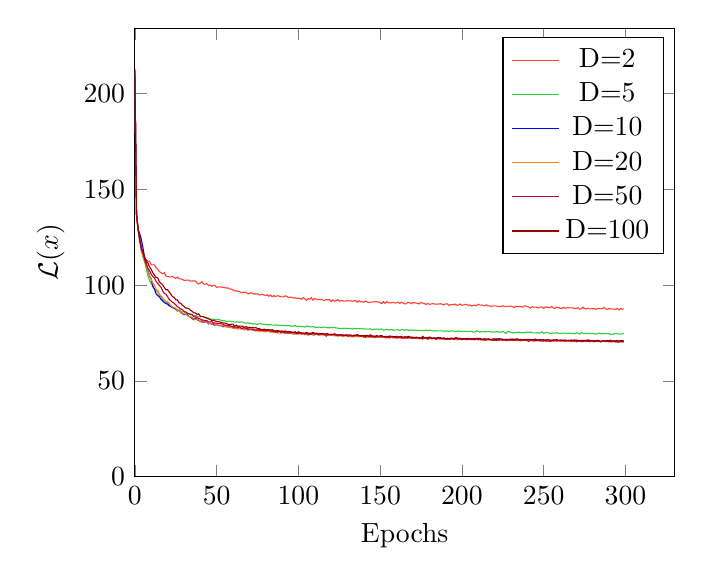
\begin{tikzpicture}\begin{axis}    [% title={Comparison of Dimension Values for Cost},
    xlabel={Epochs},ylabel={$\mathcal{L}(x)$},    xmin=0, xmax=330.0,ymin=0, ymax=234.178454269,]    \addplot[color=red,]    coordinates {(0,212.64562518)(1,136.790049189)(2,129.450027147)(3,124.806456646)(4,119.629016543)(5,115.866283098)(6,113.65281791)(7,113.216522466)(8,112.390473661)(9,112.459851352)(10,110.561585)(11,110.58909249)(12,110.582688959)(13,108.98578168)(14,108.174572268)(15,106.94951391)(16,106.52779971)(17,105.903768741)(18,106.490196048)(19,104.782711417)(20,104.510796273)(21,104.317927634)(22,104.268410977)(23,104.529566068)(24,103.975174047)(25,103.529354553)(26,104.223509424)(27,103.341782157)(28,103.223864885)(29,103.04055112)(30,102.511857203)(31,102.44037004)(32,102.624933264)(33,102.595905859)(34,102.056924605)(35,102.161272638)(36,102.107101718)(37,102.169749908)(38,101.139953877)(39,100.591849768)(40,101.12034163)(41,101.795387601)(42,100.565506148)(43,100.449325894)(44,100.776369449)(45,99.805602306)(46,100.013280903)(47,99.3922403648)(48,99.8124241222)(49,99.8443745006)(50,98.8423816612)(51,99.0189324119)(52,99.0970941301)(53,98.9608595831)(54,98.8333989091)(55,98.6930469444)(56,98.4971124406)(57,98.5305879628)(58,97.8677001537)(59,97.9693040328)(60,97.4770084312)(61,96.9026780007)(62,97.0764308583)(63,96.6972712846)(64,96.7026261208)(65,96.0112938621)(66,96.3034130166)(67,96.2243750139)(68,96.2673697316)(69,95.4720721852)(70,95.5351370933)(71,96.0084017944)(72,95.6774275901)(73,95.3824603826)(74,95.3175074768)(75,95.4738596552)(76,94.8010714999)(77,95.0208831926)(78,95.1377222651)(79,94.8573893877)(80,94.5328298118)(81,94.9248980435)(82,94.1536433272)(83,94.8404233482)(84,93.9009531888)(85,94.5247418768)(86,94.003690463)(87,94.4343333712)(88,94.3249619779)(89,93.9180274963)(90,93.8450731312)(91,93.9086502769)(92,94.4001156061)(93,94.0345778448)(94,93.4910698076)(95,93.7357471258)(96,93.620851052)(97,93.2118634033)(98,93.4317974992)(99,92.9778021379)(100,93.178931108)(101,93.0553935103)(102,92.6037774519)(103,93.4789959023)(104,92.8939061252)(105,92.0754372198)(106,92.9563021989)(107,92.5446649864)(108,93.3927328352)(109,92.1056706377)(110,92.9950072132)(111,92.6017806591)(112,92.3819902455)(113,92.4697180453)(114,92.4149521568)(115,92.1641739585)(116,92.02042099)(117,92.5232783647)(118,92.1915834462)(119,92.5636461709)(120,91.499622664)(121,92.2548089045)(122,91.5942985951)(123,91.8366348821)(124,92.4226245949)(125,91.5781864513)(126,91.9253713434)(127,91.8256563915)(128,91.6219063776)(129,91.6083890742)(130,91.9204267606)(131,91.7192824485)(132,91.8309332414)(133,91.6001627697)(134,91.7785151256)(135,91.9343934909)(136,90.9708414945)(137,91.8394788014)(138,91.2352882108)(139,91.3972491316)(140,91.053236084)(141,91.6676521024)(142,91.2520715193)(143,90.921548344)(144,91.0097028836)(145,91.2740852633)(146,91.2315159746)(147,91.3598694957)(148,91.3016590465)(149,91.116959173)(150,90.8034104503)(151,90.3776094263)(152,91.37105982)(153,90.459977847)(154,91.4105793762)(155,90.7973893738)(156,90.6487164862)(157,90.7972389776)(158,90.9623546531)(159,90.6492305825)(160,90.7841757202)(161,91.0368552191)(162,90.3820919384)(163,91.0561155978)(164,90.7019770119)(165,90.1748568309)(166,90.2482923057)(167,91.0781902244)(168,90.8552395491)(169,90.2778696095)(170,90.8713644132)(171,90.8574212785)(172,90.5594718933)(173,90.5203334323)(174,90.1041105929)(175,90.9452550437)(176,90.5799438199)(177,90.4445606578)(178,89.8594377136)(179,90.4176010825)(180,89.9413424336)(181,90.0970399891)(182,90.3487412054)(183,90.1685987715)(184,90.0106440666)(185,90.0788917403)(186,90.1420660817)(187,90.2814241583)(188,89.9337448814)(189,89.6335220406)(190,90.2058405998)(191,90.229971154)(192,89.4233127663)(193,89.7349503118)(194,89.8484557689)(195,89.8542760398)(196,90.0848807595)(197,89.4077824055)(198,89.7168458696)(199,90.091522307)(200,89.4497258412)(201,89.6172247592)(202,89.9387405673)(203,89.9406651445)(204,89.3606143882)(205,89.6490585882)(206,89.088557878)(207,89.4311926131)(208,89.4872697171)(209,89.221857064)(210,90.0243047541)(211,89.536120439)(212,89.5942551977)(213,89.4242223566)(214,89.2525826402)(215,89.6891998638)(216,89.0924630599)(217,89.1673583984)(218,88.8423385204)(219,89.1576703436)(220,89.1534130859)(221,89.1359509277)(222,88.7960712086)(223,88.941094187)(224,88.6995326233)(225,89.2326003057)(226,88.8880756031)(227,88.8336592657)(228,88.8789133731)(229,88.9285824793)(230,89.0151744218)(231,88.7847638356)(232,88.2256437544)(233,88.9106356118)(234,88.7218838778)(235,88.8426841042)(236,88.7913392084)(237,88.4047441101)(238,89.1131186745)(239,89.1689117987)(240,88.7673648626)(241,88.5378052035)(242,87.9620528481)(243,88.7573857672)(244,88.4587245456)(245,88.5162724165)(246,88.3751076438)(247,88.0754129999)(248,88.4787031139)(249,88.6045204995)(250,87.8536755232)(251,88.6177316284)(252,88.437724221)(253,88.4052790971)(254,88.2066417209)(255,88.8713390697)(256,87.9724222495)(257,87.8995355086)(258,88.4342787864)(259,88.268974755)(260,87.899311891)(261,87.7624074346)(262,88.4280469721)(263,87.8955852509)(264,88.0528344588)(265,88.1902413247)(266,88.0831458768)(267,88.0866466037)(268,88.1232280939)(269,87.7360985426)(270,87.8346880687)(271,88.1459167758)(272,87.4026767384)(273,87.6557292037)(274,88.5485077598)(275,87.7667722667)(276,87.4979941212)(277,87.977197113)(278,87.5508903642)(279,87.6130116272)(280,87.648626709)(281,87.6456446145)(282,87.3224346924)(283,87.8284001576)(284,87.7360886036)(285,87.74671789)(286,87.6882106365)(287,88.4206697568)(288,87.53956767)(289,87.2739833485)(290,87.8526529)(291,87.535925071)(292,87.5970885329)(293,87.4183481945)(294,87.3325238661)(295,87.8397986811)(296,87.0593926586)(297,87.8364493075)(298,87.3532575989)(299,87.6076428569)    };    \addplot[color=green,]    coordinates {(0,210.501984849)(1,137.075507604)(2,129.281337502)(3,124.670307298)(4,118.349319444)(5,114.545375671)(6,111.9949311)(7,108.483689686)(8,104.742418241)(9,102.436671475)(10,100.699877541)(11,99.6592659551)(12,97.9936723189)(13,97.0524140653)(14,96.2055522572)(15,94.8494610318)(16,93.8501225558)(17,92.5859065801)(18,91.9925247747)(19,91.100423473)(20,90.5070888727)(21,89.7772999573)(22,88.9261402546)(23,88.6802403606)(24,87.8085623446)(25,87.7236609303)(26,87.0449466428)(27,87.0122712985)(28,86.5224651822)(29,85.9470366044)(30,86.0935158053)(31,85.5794501634)(32,85.1979700401)(33,85.1442778709)(34,84.9510265281)(35,84.3852848608)(36,83.976246546)(37,84.2003873582)(38,83.8376353593)(39,83.4123169778)(40,83.4118772541)(41,83.604622123)(42,83.5064559728)(43,83.1131862432)(44,82.5573041673)(45,82.7421252858)(46,82.2595257985)(47,82.2053425321)(48,82.1005601085)(49,82.0737834376)(50,82.106804227)(51,81.9768792308)(52,81.8916197551)(53,81.331090296)(54,81.4447430559)(55,81.3403038788)(56,81.0759906145)(57,81.0545472648)(58,81.2044740434)(59,81.007102675)(60,80.9177202606)(61,80.6498646476)(62,80.734708252)(63,80.7922399556)(64,80.5605086725)(65,80.7934116086)(66,80.665143932)(67,80.3323184135)(68,80.0511437295)(69,80.3284948106)(70,80.0951102794)(71,80.0512655778)(72,79.7207394687)(73,79.6659372989)(74,79.7284209442)(75,79.4676317042)(76,79.7636759047)(77,79.8371999983)(78,79.6556122034)(79,79.5083737391)(80,79.3074531278)(81,79.2636697943)(82,79.2930197421)(83,79.3694778997)(84,79.092231695)(85,79.123703856)(86,79.1527527202)(87,79.1723667561)(88,78.9246874861)(89,79.0386757521)(90,78.8049234494)(91,78.9347836512)(92,78.8507095545)(93,78.6895934989)(94,78.8346243078)(95,78.7257290719)(96,78.4792713581)(97,78.61088596)(98,78.8161852819)(99,78.3291396887)(100,78.5983930414)(101,78.3670714569)(102,78.3264143302)(103,78.2904959523)(104,78.090738241)(105,78.6211502769)(106,78.4656384277)(107,78.3553288616)(108,78.1264351099)(109,78.3306529929)(110,77.97312208)(111,77.9854709001)(112,77.988705701)(113,78.0535845184)(114,77.813373316)(115,77.9109470645)(116,78.1250200306)(117,77.7843016052)(118,77.7414848466)(119,77.6925270705)(120,77.7898147652)(121,77.6532926872)(122,77.9439878152)(123,77.6072086196)(124,77.5368785997)(125,77.4319115309)(126,77.3784812719)(127,77.3251980452)(128,77.5103069999)(129,77.3995335249)(130,77.3553479212)(131,77.427784833)(132,77.3322245858)(133,77.0407563574)(134,77.4313127552)(135,77.1908862721)(136,77.2558485621)(137,77.2573469821)(138,77.1382824291)(139,77.2453216622)(140,77.0509434162)(141,77.1357038186)(142,77.0007127311)(143,77.0212986339)(144,77.177219488)(145,76.6698545491)(146,76.9416000019)(147,76.9459104503)(148,77.0630956962)(149,76.9116096843)(150,76.9611441734)(151,77.0762087319)(152,76.4179645122)(153,76.5954526104)(154,76.9663122281)(155,76.5431107192)(156,76.7295690294)(157,76.8492005851)(158,76.3803129578)(159,76.5865985732)(160,76.6495975494)(161,76.6690515484)(162,76.3390494399)(163,76.7323929319)(164,76.7073927793)(165,76.3065315039)(166,76.7965827526)(167,76.4679162112)(168,76.3149358021)(169,76.6054893216)(170,76.2898497634)(171,76.5383934784)(172,76.2822440546)(173,76.3573246418)(174,76.3488247681)(175,76.2088411435)(176,76.288880754)(177,76.2151406722)(178,76.5547682814)(179,76.2251662861)(180,76.5499588151)(181,76.2401910608)(182,76.2402269745)(183,75.9284913705)(184,76.2365732921)(185,76.0621616155)(186,76.095933179)(187,76.0857770608)(188,76.1040701363)(189,75.9783032781)(190,75.8970612058)(191,76.0414581299)(192,75.8832362574)(193,75.9362079065)(194,76.1279233482)(195,75.9636046462)(196,75.7527720642)(197,75.9061491533)(198,76.0593045252)(199,75.9230548304)(200,75.8052145178)(201,75.84747234)(202,75.9585491527)(203,75.6737758914)(204,75.799857906)(205,75.8544074319)(206,75.8279181047)(207,75.4626869132)(208,75.4334246757)(209,76.1175993694)(210,75.8160605275)(211,75.3820623433)(212,75.7279130762)(213,75.6446553109)(214,75.6278378227)(215,75.6822237743)(216,75.7021572599)(217,75.7327327728)(218,75.4201906932)(219,75.616132972)(220,75.4431809789)(221,75.6443736128)(222,75.6418913893)(223,75.3642416382)(224,75.5007856473)(225,75.7272929036)(226,75.2912066997)(227,74.8557698891)(228,75.6354122023)(229,75.646555689)(230,75.2526025737)(231,75.1074757385)(232,75.0593515639)(233,75.2300431616)(234,75.2383104914)(235,75.4473842135)(236,75.1380824072)(237,75.0794655609)(238,75.2648110338)(239,75.2718040882)(240,75.5252774811)(241,75.2152252267)(242,75.5597033553)(243,75.0637916288)(244,75.0717963063)(245,75.0603993086)(246,75.1080421656)(247,74.9899288802)(248,75.1213946603)(249,75.6110543199)(250,74.8033103874)(251,75.0794984783)(252,75.2843201308)(253,75.0477356581)(254,74.7610156527)(255,74.929453992)(256,74.9775204606)(257,74.8987329171)(258,75.1241829265)(259,74.8208806125)(260,74.817326674)(261,74.7231320537)(262,74.980364803)(263,74.8937613054)(264,74.7461031688)(265,74.9003012293)(266,74.8006846064)(267,74.658688729)(268,74.8256352303)(269,74.5678833632)(270,74.999543027)(271,74.9508922716)(272,74.4357467582)(273,75.1088637612)(274,74.8442000649)(275,74.8130131115)(276,74.7061365648)(277,74.6935067264)(278,74.6705164684)(279,74.7002849232)(280,74.8671345035)(281,74.4714349573)(282,74.426989649)(283,74.6264271199)(284,74.9894369715)(285,74.5697355791)(286,74.5427379123)(287,74.7578710729)(288,74.6157774561)(289,74.6708412795)(290,74.6360291915)(291,74.1683399617)(292,74.3667049061)(293,74.4849787071)(294,74.8149117973)(295,74.6043548376)(296,74.3590469777)(297,74.5105581457)(298,74.5680466947)(299,74.7613955064)    };    \addplot[color=blue,]    coordinates {(0,210.805377586)(1,137.116728529)(2,128.859737674)(3,126.882699585)(4,123.527543349)(5,119.283413377)(6,114.258773041)(7,111.363694708)(8,107.596632871)(9,104.649666693)(10,103.174246424)(11,99.2228121671)(12,97.9776563887)(13,95.3905151367)(14,94.5612316062)(15,93.8692550104)(16,92.5689438699)(17,91.7366139082)(18,90.9618677035)(19,90.2944361531)(20,90.1236234214)(21,89.1918947809)(22,88.8872610196)(23,88.2187327853)(24,87.945478585)(25,87.5157904746)(26,86.4525629911)(27,86.8669065163)(28,85.8463019631)(29,85.0825779655)(30,84.7324903176)(31,84.5373736503)(32,84.7178816362)(33,83.531367021)(34,83.4053398548)(35,82.6062086417)(36,81.924853044)(37,82.8104113978)(38,82.0791072221)(39,81.4736042092)(40,81.1106216361)(41,80.8272524678)(42,80.5497364738)(43,80.7907390109)(44,80.7951538155)(45,79.818405082)(46,79.9556618777)(47,79.7972120528)(48,79.4068537071)(49,79.1125786383)(50,79.2225243031)(51,79.0328106759)(52,78.7970121072)(53,78.8382280176)(54,78.268974547)(55,78.5370346347)(56,78.2795204648)(57,78.1833996443)(58,78.1062804898)(59,77.7715376143)(60,77.8667078816)(61,77.5529171961)(62,77.4743877619)(63,77.158035854)(64,77.4061579895)(65,77.2179792023)(66,77.2439936274)(67,76.6596198828)(68,77.2404046839)(69,76.4401885848)(70,76.7938676036)(71,76.7965398546)(72,76.5919960646)(73,76.3555091026)(74,76.4947394354)(75,76.2794761242)(76,76.0223075451)(77,76.2928421229)(78,76.2222049089)(79,76.0680673356)(80,75.7754479218)(81,76.1391630624)(82,75.7892865961)(83,75.7298967327)(84,76.0480288904)(85,75.2720735377)(86,75.3616966733)(87,75.8932360285)(88,75.4016416862)(89,75.2394439004)(90,75.2417322748)(91,75.2767940521)(92,74.9464581715)(93,75.073021913)(94,74.7422158189)(95,74.8724870439)(96,74.7574166177)(97,75.0232330184)(98,74.5517318032)(99,74.6715887174)(100,74.5199523302)(101,74.8786798026)(102,74.6074508806)(103,74.6752639008)(104,74.1762513178)(105,74.2637443542)(106,74.1469034507)(107,74.4218732314)(108,74.3959826938)(109,73.9786575664)(110,74.2916333701)(111,74.3400038355)(112,74.2114924552)(113,73.9273243644)(114,74.1721839697)(115,74.0829265525)(116,74.2963823353)(117,73.3767652477)(118,74.0375676727)(119,73.9004110024)(120,73.7683638417)(121,74.0675895552)(122,73.9856854525)(123,73.6399375638)(124,73.5326794087)(125,73.5831799524)(126,73.9530765325)(127,73.351258649)(128,73.8997176014)(129,73.7914783616)(130,73.3225152935)(131,73.6086916698)(132,73.3898071983)(133,73.1948840748)(134,73.5019721499)(135,73.3955278778)(136,73.3245137787)(137,73.4736843109)(138,73.2816038305)(139,73.5074686987)(140,73.4485437636)(141,72.6507272061)(142,73.1803403473)(143,72.9454844388)(144,73.1157070923)(145,73.2377040586)(146,73.2773954357)(147,73.3195385326)(148,72.9746385956)(149,73.1594836703)(150,72.8340458263)(151,72.7832887615)(152,72.9845461134)(153,72.7136743372)(154,73.0008097354)(155,72.873502225)(156,72.6611200298)(157,73.0716532412)(158,72.9241616683)(159,73.0377799364)(160,72.854239169)(161,72.6062628243)(162,72.6800379666)(163,72.728583922)(164,72.3782882621)(165,72.7541693462)(166,72.2774318071)(167,72.4181261167)(168,72.6175854562)(169,72.4200798035)(170,72.7006170932)(171,72.4649362668)(172,72.3676314337)(173,72.2532235787)(174,72.3197823334)(175,72.2944328724)(176,72.7332879223)(177,72.2654542819)(178,72.228600124)(179,72.0361454496)(180,72.2510664714)(181,72.141515496)(182,72.1215873163)(183,72.4423155767)(184,72.1798284773)(185,72.4754714064)(186,72.0542878793)(187,72.5016117096)(188,71.9982482286)(189,72.1277138034)(190,71.9718277324)(191,72.2027148784)(192,71.8538428983)(193,72.0882627869)(194,72.1624921695)(195,71.738991831)(196,72.5394513148)(197,71.7041123546)(198,71.7370714569)(199,71.8832234747)(200,71.8390793055)(201,72.0583731495)(202,71.7663406372)(203,72.1200838887)(204,71.8821543746)(205,71.6936623452)(206,71.7386560544)(207,71.735013504)(208,71.7341114114)(209,72.1664496404)(210,71.8764752059)(211,72.0868402585)(212,71.6658541315)(213,71.7407638758)(214,71.8993235709)(215,71.5313149123)(216,71.8992809157)(217,71.6577984827)(218,71.6788152937)(219,71.659934734)(220,71.3898347751)(221,71.8588566451)(222,71.8568906403)(223,71.9123310991)(224,71.8601500286)(225,71.397764095)(226,71.2743127649)(227,71.5866728835)(228,71.584455504)(229,71.5629575625)(230,71.5612635318)(231,71.7805418673)(232,71.5455781625)(233,71.6698658198)(234,71.4797457955)(235,71.2211938477)(236,71.6869631195)(237,71.265167916)(238,71.4069093739)(239,71.3827942727)(240,71.4787065125)(241,71.4591339319)(242,71.2523995139)(243,71.3399791995)(244,71.4316796181)(245,71.829281852)(246,71.0685124068)(247,71.3249252111)(248,71.4583506983)(249,71.1087824943)(250,71.2524101188)(251,71.0987912126)(252,71.0407142917)(253,71.2507783647)(254,71.1633548043)(255,71.0380099834)(256,71.2570751398)(257,71.3968035126)(258,70.8929305406)(259,71.0093754508)(260,71.1997750785)(261,71.1378930248)(262,70.8190575201)(263,71.0119934984)(264,71.0426097801)(265,70.9170135498)(266,71.1692184587)(267,70.8931625713)(268,71.1996928683)(269,71.4163565202)(270,70.4015319131)(271,71.029079361)(272,70.8215114732)(273,70.8611870575)(274,71.122573589)(275,71.0621153398)(276,70.6541871019)(277,71.3613972196)(278,71.0020488392)(279,71.0694339475)(280,70.8212981137)(281,70.8612864408)(282,70.7644188482)(283,71.1742059812)(284,70.6360337136)(285,70.5606497192)(286,70.8101563679)(287,70.8258729553)(288,70.7642208169)(289,71.1440361092)(290,70.8147142861)(291,71.1803513614)(292,70.6979013616)(293,70.7419972576)(294,70.8993927349)(295,70.8619057048)(296,70.6977005144)(297,71.0587973785)(298,70.8877211276)(299,70.5950963315)    };    \addplot[color=orange,]    coordinates {(0,210.067998685)(1,135.924982133)(2,128.162313316)(3,122.365900393)(4,117.321169697)(5,115.378946284)(6,112.446838864)(7,110.273829859)(8,107.225112929)(9,104.94283088)(10,103.006424144)(11,101.051688108)(12,99.9995623641)(13,97.7379589982)(14,97.2208271928)(15,95.0927515897)(16,94.4046158947)(17,93.374045535)(18,92.0970552895)(19,91.5744178009)(20,91.26135222)(21,90.4882005865)(22,89.3494713246)(23,88.4897178927)(24,88.3572992221)(25,87.8525562217)(26,86.5699448464)(27,86.7658450664)(28,86.0220187031)(29,85.3636644259)(30,85.0691066465)(31,84.8522001509)(32,84.2232303827)(33,83.5569254234)(34,83.4845186892)(35,83.1967647483)(36,82.4388994044)(37,81.9567146093)(38,82.1423571222)(39,81.8483164631)(40,80.8048564217)(41,81.8203006675)(42,80.7149843112)(43,80.6572627744)(44,80.5903736531)(45,80.136736686)(46,80.0964270366)(47,79.4371155895)(48,80.088521999)(49,79.3858214222)(50,79.2741473181)(51,78.8369503854)(52,78.6887142251)(53,78.7809480008)(54,78.8353205594)(55,78.2748225333)(56,78.2004178966)(57,78.3085963856)(58,78.0025651065)(59,77.9744016405)(60,77.4716886)(61,77.6376948825)(62,77.2191833288)(63,77.4403823228)(64,77.457765059)(65,77.2389772172)(66,76.9001133312)(67,76.9644827548)(68,76.8444026184)(69,76.3451540167)(70,76.6860837694)(71,76.985631596)(72,76.4810112485)(73,76.3770838998)(74,75.8985991253)(75,76.6630442116)(76,75.7269213243)(77,76.2843125777)(78,76.0529123757)(79,75.5861088978)(80,76.22549933)(81,75.7344876237)(82,75.9931949269)(83,75.4179362002)(84,75.532575642)(85,75.2223866619)(86,75.8430100874)(87,74.9378965759)(88,75.395146956)(89,74.8168042547)(90,75.1678382596)(91,75.0309718461)(92,75.0199485224)(93,75.2028841816)(94,74.7833815488)(95,75.2199762587)(96,74.6280482136)(97,74.2619567247)(98,74.9425719244)(99,74.9164593228)(100,74.5682100469)(101,74.4179598028)(102,74.377331758)(103,74.5857282188)(104,74.1685173659)(105,74.4809372156)(106,73.7183423545)(107,74.2812943476)(108,74.2187140031)(109,74.4443210186)(110,73.9411229012)(111,74.3093142007)(112,73.9010637665)(113,73.9294226907)(114,74.1067575906)(115,74.2201416917)(116,73.7519722678)(117,73.8029774059)(118,73.9551397844)(119,73.6798677479)(120,73.7457054485)(121,73.8178698522)(122,73.5380041851)(123,73.4702351587)(124,73.7084370561)(125,73.5073988412)(126,73.4265007088)(127,73.2588257183)(128,73.5227523942)(129,73.5504966042)(130,73.4830147414)(131,73.6048667145)(132,72.9733215818)(133,73.1291408123)(134,72.9092477902)(135,73.530682373)(136,73.1148989591)(137,73.0349337422)(138,73.2787869609)(139,73.2421035489)(140,72.6470006561)(141,73.1254089078)(142,72.8462848594)(143,72.9474872658)(144,72.9827051128)(145,72.6077140461)(146,72.6293927141)(147,72.6594016127)(148,72.8551838199)(149,72.9122679624)(150,72.8462239005)(151,72.6652156552)(152,72.6997789071)(153,72.5827100997)(154,72.3626133243)(155,72.7704119249)(156,72.2998460458)(157,72.9624353652)(158,72.3118800215)(159,72.5633028412)(160,72.2252251018)(161,72.6700037453)(162,72.5253759349)(163,72.2390390015)(164,72.3768651511)(165,72.37757164)(166,72.3180823309)(167,72.3214420665)(168,72.5228073259)(169,72.3010631908)(170,72.0201938629)(171,72.2315172369)(172,72.3154453278)(173,72.1195651592)(174,71.8384674558)(175,72.471930438)(176,71.5810544517)(177,72.3934994021)(178,72.3483094996)(179,71.6023356628)(180,72.1951685403)(181,72.0268935325)(182,71.8780494066)(183,72.495882395)(184,71.8206502325)(185,72.1004072432)(186,72.0318539984)(187,71.8243254436)(188,71.8782419794)(189,71.5088406927)(190,71.672149249)(191,71.6986189894)(192,71.8458012598)(193,71.8815737221)(194,71.8216658089)(195,71.8777112233)(196,71.8074403867)(197,71.4608718456)(198,71.5143265048)(199,71.7370192996)(200,71.5109205697)(201,71.6101569783)(202,71.6200373563)(203,71.3979359852)(204,71.5890264338)(205,71.7003530051)(206,71.6171399689)(207,71.6297502483)(208,71.357931366)(209,71.7080817413)(210,71.5355818523)(211,71.4957586809)(212,71.4540012845)(213,71.3020967102)(214,71.7917720448)(215,71.188479746)(216,71.2686520316)(217,71.371897042)(218,71.7548731093)(219,71.4140290763)(220,71.1514096139)(221,71.4310161452)(222,71.1650571442)(223,71.2706152691)(224,71.6830214414)(225,70.915824148)(226,71.4493759086)(227,70.9761279158)(228,71.0877371563)(229,71.565141123)(230,71.0794142844)(231,71.2863718484)(232,70.9661503116)(233,71.0355113914)(234,71.0188234017)(235,71.1096931319)(236,71.113998316)(237,71.2431414101)(238,71.1387946458)(239,71.0805060647)(240,70.8092944683)(241,70.9747370217)(242,71.1794044009)(243,71.0321707153)(244,70.9970620866)(245,70.897882954)(246,70.8474617282)(247,71.081367888)(248,70.8767741463)(249,70.9309477165)(250,70.9230121474)(251,70.6240361855)(252,70.9061814464)(253,71.0331926103)(254,71.0194979442)(255,70.7929125907)(256,70.8274236367)(257,70.8451274594)(258,70.8660537442)(259,71.0744285098)(260,70.9579298054)(261,70.664812851)(262,70.9925811976)(263,70.6772500194)(264,70.899464361)(265,70.7725664659)(266,70.7583813962)(267,70.4356981312)(268,70.5925863509)(269,70.4825072757)(270,70.9462791235)(271,70.9600786868)(272,70.6372254874)(273,70.4675903598)(274,70.5070909257)(275,70.5083206593)(276,70.7750220351)(277,70.6195004342)(278,70.4290041213)(279,71.0901097731)(280,70.3589060003)(281,70.467044428)(282,70.7747598683)(283,70.8541592754)(284,70.572219058)(285,70.3026625408)(286,70.5957660814)(287,70.5955959667)(288,70.6720675104)(289,70.4583931871)(290,70.3036518236)(291,70.4643600672)(292,70.2936555342)(293,70.5787976352)(294,70.1761015736)(295,70.1782268663)(296,70.4880830037)(297,70.5506308122)(298,70.1181903146)(299,70.2723682612)    };    \addplot[color=purple,]    coordinates {(0,212.889503881)(1,136.69067473)(2,128.82833134)(3,124.040854936)(4,118.690849804)(5,116.909000924)(6,113.013927626)(7,111.075254586)(8,108.798369917)(9,107.562806091)(10,105.667284851)(11,104.449745872)(12,103.738867798)(13,101.913222407)(14,100.880470165)(15,99.7707582092)(16,98.9113952359)(17,96.9467745001)(18,95.6420740024)(19,95.3488831676)(20,93.9665334251)(21,92.4877756431)(22,91.8431637018)(23,91.0363048068)(24,90.5232136397)(25,89.7399208069)(26,88.7281854803)(27,88.1798480225)(28,87.5367355208)(29,87.3209809875)(30,86.2576438349)(31,86.0276815102)(32,85.4221434021)(33,85.0303677923)(34,84.5800309337)(35,84.7152453891)(36,83.5131790022)(37,83.4104959453)(38,83.1304513758)(39,82.4841615989)(40,82.3764996546)(41,81.7875932936)(42,81.7060721588)(43,81.3806930681)(44,81.4111268546)(45,80.838586731)(46,80.7406091725)(47,81.017188041)(48,80.2124638228)(49,80.2271451361)(50,80.0896083138)(51,79.8871128637)(52,79.8942684867)(53,79.7550364408)(54,79.538298645)(55,79.0118305414)(56,79.0969413133)(57,78.7534699735)(58,78.9117192979)(59,78.3776827171)(60,78.4891304779)(61,78.0464635398)(62,78.1325949721)(63,77.9003106967)(64,78.1739014712)(65,77.4500395133)(66,77.6281871865)(67,77.6110464131)(68,77.474847426)(69,77.2124328683)(70,77.1030504678)(71,76.9742827121)(72,77.1269824912)(73,76.453514002)(74,76.6268032559)(75,76.3920169484)(76,77.0279490245)(77,76.1911592518)(78,76.1912690319)(79,76.4120253546)(80,76.3616653512)(81,76.4200014773)(82,76.1013489741)(83,76.1299544941)(84,75.9456712133)(85,75.8474544456)(86,75.9958151453)(87,75.4516047114)(88,75.9606080211)(89,75.7825870514)(90,75.4166851807)(91,75.2730201028)(92,75.5633785178)(93,75.3926641221)(94,75.1231771504)(95,75.3425059509)(96,75.2793357017)(97,75.42107236)(98,75.0752778209)(99,75.1563735268)(100,74.7741940308)(101,75.0860549094)(102,74.687021852)(103,74.6451232633)(104,74.4814327032)(105,74.6204650948)(106,74.6206243688)(107,74.3239216544)(108,74.2764617642)(109,74.8516898277)(110,74.3182112052)(111,74.7670684121)(112,74.3290488018)(113,74.5695130088)(114,74.3323224362)(115,74.6895237246)(116,74.0510518993)(117,73.9067425815)(118,74.0074700442)(119,74.1338988495)(120,74.0175181926)(121,74.1761847895)(122,74.0235229562)(123,73.9181140345)(124,73.8457655473)(125,73.8702288749)(126,74.0162856362)(127,73.6437659316)(128,73.4565949943)(129,73.9170945116)(130,73.5467081313)(131,73.4937463864)(132,73.5905630146)(133,73.353295621)(134,73.6264864766)(135,73.5908654092)(136,73.5732003923)(137,73.4532649994)(138,73.2716727794)(139,73.465524188)(140,73.112097598)(141,73.2420930204)(142,73.5635126287)(143,73.3090762398)(144,72.9897125105)(145,73.2172430489)(146,73.1516952931)(147,72.7228497869)(148,73.0782187098)(149,73.1016768508)(150,73.4024589885)(151,72.880766879)(152,73.0312317588)(153,72.7873863844)(154,72.9423721105)(155,72.5628787509)(156,72.8360966284)(157,73.047174426)(158,72.8167339325)(159,72.6396780465)(160,73.0304298262)(161,72.4665298601)(162,72.6912430434)(163,72.5760772358)(164,72.4846100339)(165,72.459022411)(166,72.5838312045)(167,72.6003749293)(168,72.5145784413)(169,72.3569016474)(170,72.3737294076)(171,72.4213695249)(172,72.3710491943)(173,72.4755430534)(174,72.4657969249)(175,72.2095316592)(176,72.0375349288)(177,72.5440174311)(178,72.5334384502)(179,71.8655854936)(180,72.008425508)(181,72.254446425)(182,72.1637018724)(183,72.2237791096)(184,71.714810257)(185,71.9142984702)(186,72.0176052856)(187,72.0815261771)(188,72.0838776606)(189,72.2727386128)(190,71.688610285)(191,71.8585383883)(192,71.8177259757)(193,71.7062380357)(194,72.1454219471)(195,71.6026708776)(196,72.2864398055)(197,71.9247254597)(198,71.868394928)(199,71.8450078375)(200,71.4535544239)(201,71.8534567261)(202,71.670494683)(203,71.8755769626)(204,71.7016650391)(205,71.6363452565)(206,71.504623205)(207,71.5315711698)(208,71.587473741)(209,71.8978508828)(210,71.4103687564)(211,71.70563883)(212,71.3756308677)(213,71.5474994174)(214,71.1844528337)(215,71.60504733)(216,71.8060398934)(217,71.4310690862)(218,71.3169561282)(219,71.1020025912)(220,71.425415476)(221,71.1148356559)(222,71.7071190435)(223,71.1754220234)(224,71.483830067)(225,71.261985321)(226,71.4267416937)(227,71.0780576116)(228,71.5027765656)(229,71.1248665203)(230,71.3434074541)(231,71.0519401204)(232,71.3568696039)(233,71.2187969555)(234,71.4516134782)(235,71.2335008032)(236,70.9221232674)(237,71.3969466123)(238,70.9965213568)(239,71.3100876895)(240,71.1295058164)(241,70.6539552723)(242,71.2394960577)(243,70.9955520907)(244,70.8132880679)(245,71.0490945296)(246,71.1247871052)(247,71.0870736417)(248,70.7841236739)(249,70.9903914504)(250,70.7095126967)(251,71.2655674189)(252,70.6899923706)(253,70.8693695623)(254,70.6116099063)(255,70.951697138)(256,70.8354414368)(257,71.0545902252)(258,70.8714400898)(259,70.8538174022)(260,70.822078039)(261,70.8707302163)(262,70.8950232905)(263,70.7760084395)(264,70.7706362083)(265,70.9704128127)(266,70.7572787822)(267,70.7819294947)(268,70.9383078766)(269,70.7281015916)(270,70.8945835599)(271,70.482622972)(272,70.93528905)(273,70.5277008334)(274,70.5941716211)(275,70.8907409599)(276,70.6606239388)(277,70.7143197632)(278,70.4889673545)(279,70.7734613106)(280,70.716083048)(281,70.5357097002)(282,70.6280721283)(283,70.5701076577)(284,70.6263676938)(285,70.4352469635)(286,70.7839288816)(287,70.8557285656)(288,70.4485128229)(289,70.8420001637)(290,70.5595037981)(291,70.5228122572)(292,70.6055964106)(293,70.5968888716)(294,70.4848312725)(295,70.6190093855)(296,70.1423300726)(297,70.5032779763)(298,70.5609679066)(299,70.6179385029)    };    \addplot[color=crimson,]    coordinates {(0,212.039563182)(1,137.227005865)(2,129.614564015)(3,122.868323142)(4,119.571938144)(5,116.697059687)(6,114.658347473)(7,112.527611417)(8,111.440707689)(9,109.471019107)(10,108.22395591)(11,106.433720398)(12,105.239981468)(13,104.024576014)(14,103.772119127)(15,101.646527363)(16,100.905797577)(17,100.20180757)(18,98.7593887052)(19,97.5801294084)(20,97.5575055764)(21,96.3992757901)(22,95.2872680664)(23,93.9911086065)(24,93.6356017512)(25,92.3592711986)(26,92.2598874318)(27,90.7334927923)(28,90.4955191456)(29,89.5533440052)(30,88.9449502563)(31,88.0546641541)(32,88.0069049766)(33,87.6846243841)(34,86.8078676813)(35,86.3173411421)(36,85.543703433)(37,85.4867595256)(38,84.7009303353)(39,85.0167525274)(40,83.7460846363)(41,83.6698393596)(42,83.4445797799)(43,83.0411663541)(44,82.9096408913)(45,82.3510414956)(46,82.0608427637)(47,81.5545689323)(48,81.5605580902)(49,81.3109250849)(50,81.0572958443)(51,80.9268129037)(52,80.7258593473)(53,80.3824426686)(54,80.2055065294)(55,80.1646096663)(56,79.9869374015)(57,79.5170462591)(58,79.4061609095)(59,79.5656501007)(60,79.6308617332)(61,78.5143985124)(62,79.135577455)(63,78.3613404638)(64,78.6407981387)(65,78.563548695)(66,78.4910784427)(67,77.925945601)(68,78.3036572543)(69,77.9039735205)(70,77.9748676786)(71,77.7790186865)(72,77.8952567291)(73,77.596546721)(74,77.8247525649)(75,77.2450709603)(76,77.3437627896)(77,76.8722628715)(78,76.599724565)(79,77.0143345434)(80,76.8284113312)(81,76.635512078)(82,76.809213673)(83,76.5110565532)(84,76.7733340454)(85,76.159373814)(86,75.9849719654)(87,76.1730693193)(88,76.1426014363)(89,75.6682129739)(90,76.1217581177)(91,75.7681585347)(92,76.0921120314)(93,75.3710738789)(94,75.7868552745)(95,75.6391721968)(96,75.4986325628)(97,75.1434716936)(98,75.6404488512)(99,74.6438331188)(100,75.6185196408)(101,75.2318935047)(102,74.9748832703)(103,75.0609959481)(104,74.8513715709)(105,75.3014293046)(106,74.8140919841)(107,74.8457119404)(108,74.9727545097)(109,75.241271182)(110,74.7714003268)(111,74.9243031797)(112,74.4076462694)(113,74.6716630624)(114,74.6927879611)(115,74.5755828094)(116,74.4379206016)(117,74.6187052155)(118,74.5941385373)(119,74.141126494)(120,74.3427397988)(121,74.2087947776)(122,74.5707944072)(123,74.3412156053)(124,73.7706280101)(125,74.192972856)(126,73.9348603613)(127,74.026331364)(128,73.691987166)(129,73.8850137398)(130,74.0069591245)(131,74.0306104209)(132,74.0371748491)(133,73.4270824224)(134,73.9323885207)(135,73.7935875841)(136,74.1767524858)(137,73.7194287248)(138,73.5894774212)(139,73.4787757249)(140,73.5292327742)(141,73.6168738348)(142,73.734774274)(143,73.342374226)(144,74.0275036899)(145,73.5368975067)(146,73.2592835097)(147,73.1974846441)(148,73.7065324124)(149,73.0416785431)(150,73.6097421473)(151,73.6058541454)(152,73.0523033281)(153,73.1077828425)(154,73.2408514751)(155,73.1611174566)(156,73.3866937464)(157,73.2324635315)(158,73.223810508)(159,72.8410156389)(160,73.2730692707)(161,72.9142342862)(162,73.0589042386)(163,73.2076397636)(164,72.702815635)(165,73.0443814572)(166,72.8409559493)(167,73.2653859295)(168,73.0079451197)(169,72.7579323439)(170,72.7907337674)(171,72.5297621918)(172,72.8243227941)(173,72.5943514182)(174,72.4342909588)(175,72.1721242038)(176,73.2465561191)(177,72.4238556671)(178,72.5926984891)(179,72.4761038208)(180,72.8798136278)(181,72.5854214478)(182,72.2764034133)(183,72.4566061263)(184,72.1982383034)(185,72.5277849579)(186,72.7088948337)(187,72.1059343442)(188,72.2482518075)(189,72.4276114238)(190,71.8815495439)(191,72.0862786518)(192,72.0678002305)(193,72.2957406963)(194,72.1430504608)(195,72.1484981537)(196,71.9697526204)(197,72.5720690987)(198,71.9797823056)(199,72.2632491996)(200,71.9456255895)(201,71.8932656652)(202,72.080543636)(203,71.7892183893)(204,72.2095629259)(205,71.7839186928)(206,72.0567432195)(207,72.0026570337)(208,71.9424785406)(209,72.1611479464)(210,72.1670975009)(211,72.0808817083)(212,71.7657454473)(213,71.5818119327)(214,71.9939413799)(215,71.5670192719)(216,71.7554188746)(217,71.6532582578)(218,71.5559408847)(219,71.7905417494)(220,72.0833369515)(221,71.2988774248)(222,71.8309216031)(223,71.8537068038)(224,71.747578451)(225,71.7339050501)(226,71.6105525069)(227,71.7546853638)(228,71.3571602492)(229,71.6606266507)(230,71.8033929374)(231,71.6524653071)(232,71.6965953619)(233,71.7416812897)(234,71.9445179402)(235,71.4681651237)(236,71.5460668182)(237,71.5479721347)(238,71.4190080331)(239,71.6026788469)(240,71.6197561299)(241,71.6569667608)(242,71.6510816678)(243,71.4505215732)(244,71.6025352062)(245,71.1539069505)(246,71.309879088)(247,71.4973060261)(248,71.3534587028)(249,71.4245876936)(250,71.4703724601)(251,71.1119898709)(252,71.5169133204)(253,71.4497759802)(254,71.1549646412)(255,71.2602478374)(256,71.3688519287)(257,71.2276049666)(258,71.6382891152)(259,71.107729943)(260,71.2443089294)(261,71.3530235915)(262,71.1255810408)(263,71.3901048071)(264,71.0870995331)(265,71.1928002999)(266,71.0295605261)(267,71.3385529744)(268,70.9274197873)(269,71.0613703641)(270,71.2191394043)(271,71.1685913017)(272,71.0013334586)(273,71.1794925759)(274,70.8293097409)(275,71.0646055256)(276,71.1837904843)(277,70.9545514263)(278,71.1789379605)(279,70.8328126526)(280,71.0099153484)(281,70.8474416976)(282,70.9677443001)(283,70.8127647608)(284,70.9805190485)(285,70.5329126323)(286,70.8466603505)(287,70.9979537409)(288,70.7751597387)(289,70.8110449774)(290,70.6825756767)(291,71.0729032066)(292,70.6829895644)(293,70.902476876)(294,70.6805907024)(295,70.938482125)(296,70.8477972551)(297,70.9155728427)(298,70.8201013392)(299,70.7504443637)    };    \legend{D=2,D=5,D=10,D=20,D=50,D=100,}\end{axis}\end{tikzpicture}\\}
  \caption{Latent Dimensionality}
  \label{fig:latdimcost}
\end{wrapfigure}
Finally, we were interested in determining how the choice of latent space dimensionality affected the training of our model. As described previously, the number of latent dimensions, $n_z$ is given by the number of nodes in the stochastic layer of the model.
\par To experiment with this parameter, we trained multiple Importance Weighted VAEs with dimensionality ${n_z \in \{2,5,10,20,50,100\}}$. See the effect of dimensionality on training in Figure \ref{fig:latdimcost}. Our experiments show that models with 2 or 5 latent dimensions were not trained as successfully as models with higher latent dimensions. Further, it is interesting to note that all models with $n_z\geq10$ converged to the same log-likelihood bound. This suggests to us that the additional latent dimensionality was not useful for learning latent representations of the MNIST data. In fact, $n_z=10$ converged slightly faster than higher latent dimensional models, further suggesting that the additional dimensions were superfluous to training.
\par We were particularly interested in this question of latent space dimensionality. It is especially suggestive that models with $n_z\geq10$ perform identically, given that there are 10 classes of digits in MNIST. This motivates our inquiry for the next section where we explore usefulness of latent dimensions by describing their activity.

\section{Latent Dimension Activity}
\subsection{Activity Metric}
In the previous sections we discussed latent dimension activity. Here we define it explicitly, using a method described by Burda, Grosse, \& Salakhutdinov \cite{Burda2016}. Given that the distribution parameters of nodes in the latent space combine to form the latent representation of the data, the authors observed that if the parameters remain the same or very similar while encoding  all data in the training set, then the contribution of those nodes and their corresponding latent dimensions to the representation of the data is minor. As such, they defined a measurement of latent dimension activity from the variance of the expected value of the latent distribution across each dimension:
\begin{align}
  Cov_{\textbf{x}}\left(\mathbb{E}_{u~q(u|\textbf{x})}[u]\right)>\epsilon
  \label{eq:ACTIVITYMET}
\end{align}
\par Where $u$ represents a single dimension in the latent space, $q$ is the generative distribution of the encoder network $q_\phi$, and $\epsilon$ is a threshold value. Any dimension whose activity (represented by the left-hand side of the equation) exceeds $\epsilon$ is defined as ``active`` for the purposes of our experiment. In the experiment from \cite{Burda2016}, an activation of $\epsilon=10^{-2}$ was used, but for this experiment a higher threshold of $\epsilon=10^{-1}$ proved to be more useful as many dimensions surpassed this lower threshold with random variation. The effect of the additional methods described previously, averaged over multiple trials with a 50 dimensional VAE, can be seen in the Figure \ref{fig:activities}.
\begin{figure}[h]
\captionsetup[subfigure]{justification=centering}
  \centering
  \begin{subfigure}[t]{0.3\textwidth}
    \resizebox{\linewidth}{!}{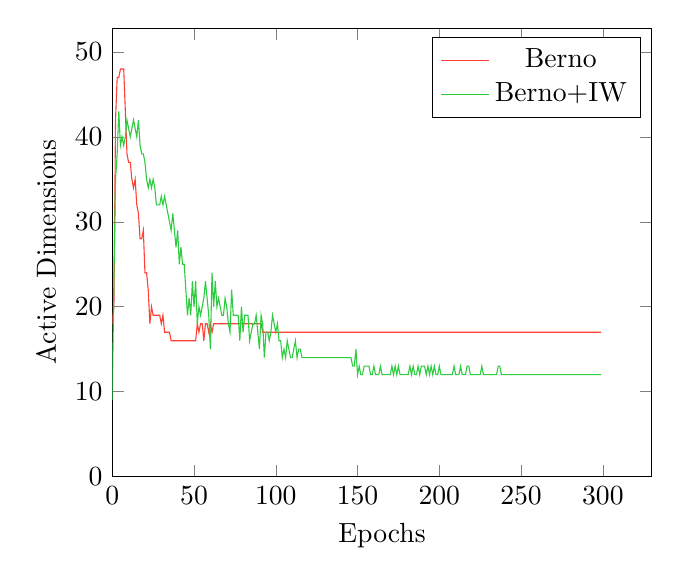
\begin{tikzpicture}\begin{axis}    [% title={Comparison of Vanilla and Importance Weighted Activity},
    xlabel={Epochs},ylabel={Active Dimensions},    xmin=0, xmax=330.0,ymin=0, ymax=52.8,]    \addplot[color=red,]    coordinates {(0,18.0)(1,20.0)(2,42.0)(3,47.0)(4,47.0)(5,48.0)(6,48.0)(7,48.0)(8,43.0)(9,38.0)(10,37.0)(11,37.0)(12,35.0)(13,34.0)(14,35.0)(15,32.0)(16,31.0)(17,28.0)(18,28.0)(19,29.0)(20,24.0)(21,24.0)(22,22.0)(23,18.0)(24,20.0)(25,19.0)(26,19.0)(27,19.0)(28,19.0)(29,19.0)(30,18.0)(31,19.0)(32,17.0)(33,17.0)(34,17.0)(35,17.0)(36,16.0)(37,16.0)(38,16.0)(39,16.0)(40,16.0)(41,16.0)(42,16.0)(43,16.0)(44,16.0)(45,16.0)(46,16.0)(47,16.0)(48,16.0)(49,16.0)(50,16.0)(51,16.0)(52,18.0)(53,17.0)(54,18.0)(55,18.0)(56,16.0)(57,18.0)(58,18.0)(59,17.0)(60,18.0)(61,17.0)(62,18.0)(63,18.0)(64,18.0)(65,18.0)(66,18.0)(67,18.0)(68,18.0)(69,18.0)(70,18.0)(71,18.0)(72,18.0)(73,18.0)(74,18.0)(75,18.0)(76,18.0)(77,18.0)(78,18.0)(79,18.0)(80,18.0)(81,18.0)(82,18.0)(83,18.0)(84,18.0)(85,18.0)(86,18.0)(87,18.0)(88,18.0)(89,18.0)(90,18.0)(91,18.0)(92,17.0)(93,17.0)(94,17.0)(95,17.0)(96,17.0)(97,17.0)(98,17.0)(99,17.0)(100,17.0)(101,17.0)(102,17.0)(103,17.0)(104,17.0)(105,17.0)(106,17.0)(107,17.0)(108,17.0)(109,17.0)(110,17.0)(111,17.0)(112,17.0)(113,17.0)(114,17.0)(115,17.0)(116,17.0)(117,17.0)(118,17.0)(119,17.0)(120,17.0)(121,17.0)(122,17.0)(123,17.0)(124,17.0)(125,17.0)(126,17.0)(127,17.0)(128,17.0)(129,17.0)(130,17.0)(131,17.0)(132,17.0)(133,17.0)(134,17.0)(135,17.0)(136,17.0)(137,17.0)(138,17.0)(139,17.0)(140,17.0)(141,17.0)(142,17.0)(143,17.0)(144,17.0)(145,17.0)(146,17.0)(147,17.0)(148,17.0)(149,17.0)(150,17.0)(151,17.0)(152,17.0)(153,17.0)(154,17.0)(155,17.0)(156,17.0)(157,17.0)(158,17.0)(159,17.0)(160,17.0)(161,17.0)(162,17.0)(163,17.0)(164,17.0)(165,17.0)(166,17.0)(167,17.0)(168,17.0)(169,17.0)(170,17.0)(171,17.0)(172,17.0)(173,17.0)(174,17.0)(175,17.0)(176,17.0)(177,17.0)(178,17.0)(179,17.0)(180,17.0)(181,17.0)(182,17.0)(183,17.0)(184,17.0)(185,17.0)(186,17.0)(187,17.0)(188,17.0)(189,17.0)(190,17.0)(191,17.0)(192,17.0)(193,17.0)(194,17.0)(195,17.0)(196,17.0)(197,17.0)(198,17.0)(199,17.0)(200,17.0)(201,17.0)(202,17.0)(203,17.0)(204,17.0)(205,17.0)(206,17.0)(207,17.0)(208,17.0)(209,17.0)(210,17.0)(211,17.0)(212,17.0)(213,17.0)(214,17.0)(215,17.0)(216,17.0)(217,17.0)(218,17.0)(219,17.0)(220,17.0)(221,17.0)(222,17.0)(223,17.0)(224,17.0)(225,17.0)(226,17.0)(227,17.0)(228,17.0)(229,17.0)(230,17.0)(231,17.0)(232,17.0)(233,17.0)(234,17.0)(235,17.0)(236,17.0)(237,17.0)(238,17.0)(239,17.0)(240,17.0)(241,17.0)(242,17.0)(243,17.0)(244,17.0)(245,17.0)(246,17.0)(247,17.0)(248,17.0)(249,17.0)(250,17.0)(251,17.0)(252,17.0)(253,17.0)(254,17.0)(255,17.0)(256,17.0)(257,17.0)(258,17.0)(259,17.0)(260,17.0)(261,17.0)(262,17.0)(263,17.0)(264,17.0)(265,17.0)(266,17.0)(267,17.0)(268,17.0)(269,17.0)(270,17.0)(271,17.0)(272,17.0)(273,17.0)(274,17.0)(275,17.0)(276,17.0)(277,17.0)(278,17.0)(279,17.0)(280,17.0)(281,17.0)(282,17.0)(283,17.0)(284,17.0)(285,17.0)(286,17.0)(287,17.0)(288,17.0)(289,17.0)(290,17.0)(291,17.0)(292,17.0)(293,17.0)(294,17.0)(295,17.0)(296,17.0)(297,17.0)(298,17.0)(299,17.0)    };    \addplot[color=green,]    coordinates {(0,9.0)(1,23.0)(2,35.0)(3,38.0)(4,43.0)(5,39.0)(6,40.0)(7,39.0)(8,40.0)(9,42.0)(10,41.0)(11,40.0)(12,41.0)(13,42.0)(14,41.0)(15,40.0)(16,42.0)(17,39.0)(18,38.0)(19,38.0)(20,37.0)(21,35.0)(22,34.0)(23,35.0)(24,34.0)(25,35.0)(26,34.0)(27,32.0)(28,32.0)(29,32.0)(30,33.0)(31,32.0)(32,33.0)(33,32.0)(34,31.0)(35,30.0)(36,29.0)(37,31.0)(38,29.0)(39,27.0)(40,29.0)(41,25.0)(42,27.0)(43,25.0)(44,25.0)(45,22.0)(46,19.0)(47,21.0)(48,19.0)(49,23.0)(50,20.0)(51,23.0)(52,18.0)(53,20.0)(54,19.0)(55,20.0)(56,21.0)(57,23.0)(58,21.0)(59,19.0)(60,15.0)(61,24.0)(62,20.0)(63,23.0)(64,20.0)(65,21.0)(66,20.0)(67,19.0)(68,19.0)(69,21.0)(70,20.0)(71,18.0)(72,17.0)(73,22.0)(74,19.0)(75,19.0)(76,19.0)(77,19.0)(78,16.0)(79,20.0)(80,17.0)(81,19.0)(82,19.0)(83,19.0)(84,16.0)(85,17.0)(86,18.0)(87,18.0)(88,19.0)(89,17.0)(90,15.0)(91,19.0)(92,18.0)(93,14.0)(94,17.0)(95,17.0)(96,16.0)(97,17.0)(98,19.0)(99,18.0)(100,17.0)(101,18.0)(102,16.0)(103,16.0)(104,14.0)(105,15.0)(106,14.0)(107,16.0)(108,15.0)(109,14.0)(110,14.0)(111,15.0)(112,16.0)(113,14.0)(114,15.0)(115,15.0)(116,14.0)(117,14.0)(118,14.0)(119,14.0)(120,14.0)(121,14.0)(122,14.0)(123,14.0)(124,14.0)(125,14.0)(126,14.0)(127,14.0)(128,14.0)(129,14.0)(130,14.0)(131,14.0)(132,14.0)(133,14.0)(134,14.0)(135,14.0)(136,14.0)(137,14.0)(138,14.0)(139,14.0)(140,14.0)(141,14.0)(142,14.0)(143,14.0)(144,14.0)(145,14.0)(146,14.0)(147,13.0)(148,13.0)(149,15.0)(150,12.0)(151,13.0)(152,12.0)(153,12.0)(154,13.0)(155,13.0)(156,13.0)(157,13.0)(158,12.0)(159,12.0)(160,13.0)(161,12.0)(162,12.0)(163,12.0)(164,13.0)(165,12.0)(166,12.0)(167,12.0)(168,12.0)(169,12.0)(170,12.0)(171,13.0)(172,12.0)(173,13.0)(174,12.0)(175,13.0)(176,12.0)(177,12.0)(178,12.0)(179,12.0)(180,12.0)(181,12.0)(182,13.0)(183,12.0)(184,13.0)(185,12.0)(186,12.0)(187,13.0)(188,12.0)(189,13.0)(190,13.0)(191,13.0)(192,12.0)(193,13.0)(194,12.0)(195,13.0)(196,12.0)(197,13.0)(198,12.0)(199,12.0)(200,13.0)(201,12.0)(202,12.0)(203,12.0)(204,12.0)(205,12.0)(206,12.0)(207,12.0)(208,12.0)(209,13.0)(210,12.0)(211,12.0)(212,12.0)(213,13.0)(214,12.0)(215,12.0)(216,12.0)(217,13.0)(218,13.0)(219,12.0)(220,12.0)(221,12.0)(222,12.0)(223,12.0)(224,12.0)(225,12.0)(226,13.0)(227,12.0)(228,12.0)(229,12.0)(230,12.0)(231,12.0)(232,12.0)(233,12.0)(234,12.0)(235,12.0)(236,13.0)(237,13.0)(238,12.0)(239,12.0)(240,12.0)(241,12.0)(242,12.0)(243,12.0)(244,12.0)(245,12.0)(246,12.0)(247,12.0)(248,12.0)(249,12.0)(250,12.0)(251,12.0)(252,12.0)(253,12.0)(254,12.0)(255,12.0)(256,12.0)(257,12.0)(258,12.0)(259,12.0)(260,12.0)(261,12.0)(262,12.0)(263,12.0)(264,12.0)(265,12.0)(266,12.0)(267,12.0)(268,12.0)(269,12.0)(270,12.0)(271,12.0)(272,12.0)(273,12.0)(274,12.0)(275,12.0)(276,12.0)(277,12.0)(278,12.0)(279,12.0)(280,12.0)(281,12.0)(282,12.0)(283,12.0)(284,12.0)(285,12.0)(286,12.0)(287,12.0)(288,12.0)(289,12.0)(290,12.0)(291,12.0)(292,12.0)(293,12.0)(294,12.0)(295,12.0)(296,12.0)(297,12.0)(298,12.0)(299,12.0)    };    \legend{Berno,Berno+IW,}\end{axis}\end{tikzpicture}\\}
    \caption{Importance Weighting (IW)}
    \label{fig:iwlat}
  \end{subfigure}
  \begin{subfigure}[t]{0.3\textwidth}
    \resizebox{\linewidth}{!}{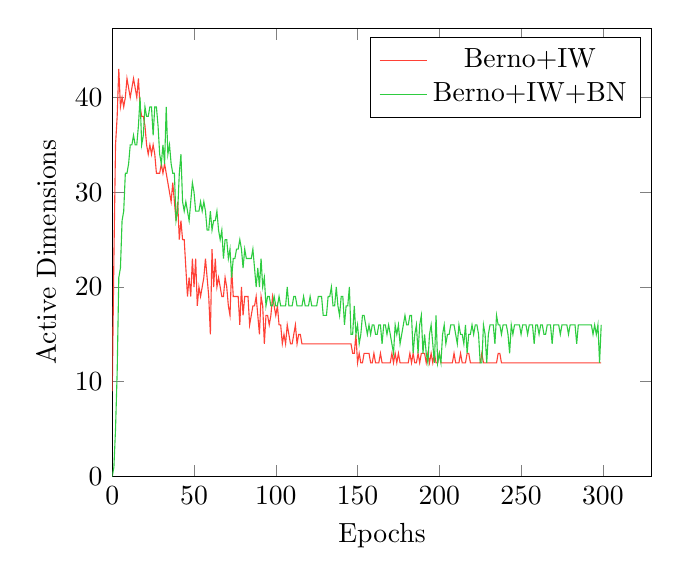
\begin{tikzpicture}\begin{axis}    [% title={Comparison of Importance Weighted and Batch Normalized for Activity},
    xlabel={Epochs},ylabel={Active Dimensions},    xmin=0, xmax=330.0,ymin=0, ymax=47.3,]    \addplot[color=red,]    coordinates {(0,9.0)(1,23.0)(2,35.0)(3,38.0)(4,43.0)(5,39.0)(6,40.0)(7,39.0)(8,40.0)(9,42.0)(10,41.0)(11,40.0)(12,41.0)(13,42.0)(14,41.0)(15,40.0)(16,42.0)(17,39.0)(18,38.0)(19,38.0)(20,37.0)(21,35.0)(22,34.0)(23,35.0)(24,34.0)(25,35.0)(26,34.0)(27,32.0)(28,32.0)(29,32.0)(30,33.0)(31,32.0)(32,33.0)(33,32.0)(34,31.0)(35,30.0)(36,29.0)(37,31.0)(38,29.0)(39,27.0)(40,29.0)(41,25.0)(42,27.0)(43,25.0)(44,25.0)(45,22.0)(46,19.0)(47,21.0)(48,19.0)(49,23.0)(50,20.0)(51,23.0)(52,18.0)(53,20.0)(54,19.0)(55,20.0)(56,21.0)(57,23.0)(58,21.0)(59,19.0)(60,15.0)(61,24.0)(62,20.0)(63,23.0)(64,20.0)(65,21.0)(66,20.0)(67,19.0)(68,19.0)(69,21.0)(70,20.0)(71,18.0)(72,17.0)(73,22.0)(74,19.0)(75,19.0)(76,19.0)(77,19.0)(78,16.0)(79,20.0)(80,17.0)(81,19.0)(82,19.0)(83,19.0)(84,16.0)(85,17.0)(86,18.0)(87,18.0)(88,19.0)(89,17.0)(90,15.0)(91,19.0)(92,18.0)(93,14.0)(94,17.0)(95,17.0)(96,16.0)(97,17.0)(98,19.0)(99,18.0)(100,17.0)(101,18.0)(102,16.0)(103,16.0)(104,14.0)(105,15.0)(106,14.0)(107,16.0)(108,15.0)(109,14.0)(110,14.0)(111,15.0)(112,16.0)(113,14.0)(114,15.0)(115,15.0)(116,14.0)(117,14.0)(118,14.0)(119,14.0)(120,14.0)(121,14.0)(122,14.0)(123,14.0)(124,14.0)(125,14.0)(126,14.0)(127,14.0)(128,14.0)(129,14.0)(130,14.0)(131,14.0)(132,14.0)(133,14.0)(134,14.0)(135,14.0)(136,14.0)(137,14.0)(138,14.0)(139,14.0)(140,14.0)(141,14.0)(142,14.0)(143,14.0)(144,14.0)(145,14.0)(146,14.0)(147,13.0)(148,13.0)(149,15.0)(150,12.0)(151,13.0)(152,12.0)(153,12.0)(154,13.0)(155,13.0)(156,13.0)(157,13.0)(158,12.0)(159,12.0)(160,13.0)(161,12.0)(162,12.0)(163,12.0)(164,13.0)(165,12.0)(166,12.0)(167,12.0)(168,12.0)(169,12.0)(170,12.0)(171,13.0)(172,12.0)(173,13.0)(174,12.0)(175,13.0)(176,12.0)(177,12.0)(178,12.0)(179,12.0)(180,12.0)(181,12.0)(182,13.0)(183,12.0)(184,13.0)(185,12.0)(186,12.0)(187,13.0)(188,12.0)(189,13.0)(190,13.0)(191,13.0)(192,12.0)(193,13.0)(194,12.0)(195,13.0)(196,12.0)(197,13.0)(198,12.0)(199,12.0)(200,13.0)(201,12.0)(202,12.0)(203,12.0)(204,12.0)(205,12.0)(206,12.0)(207,12.0)(208,12.0)(209,13.0)(210,12.0)(211,12.0)(212,12.0)(213,13.0)(214,12.0)(215,12.0)(216,12.0)(217,13.0)(218,13.0)(219,12.0)(220,12.0)(221,12.0)(222,12.0)(223,12.0)(224,12.0)(225,12.0)(226,13.0)(227,12.0)(228,12.0)(229,12.0)(230,12.0)(231,12.0)(232,12.0)(233,12.0)(234,12.0)(235,12.0)(236,13.0)(237,13.0)(238,12.0)(239,12.0)(240,12.0)(241,12.0)(242,12.0)(243,12.0)(244,12.0)(245,12.0)(246,12.0)(247,12.0)(248,12.0)(249,12.0)(250,12.0)(251,12.0)(252,12.0)(253,12.0)(254,12.0)(255,12.0)(256,12.0)(257,12.0)(258,12.0)(259,12.0)(260,12.0)(261,12.0)(262,12.0)(263,12.0)(264,12.0)(265,12.0)(266,12.0)(267,12.0)(268,12.0)(269,12.0)(270,12.0)(271,12.0)(272,12.0)(273,12.0)(274,12.0)(275,12.0)(276,12.0)(277,12.0)(278,12.0)(279,12.0)(280,12.0)(281,12.0)(282,12.0)(283,12.0)(284,12.0)(285,12.0)(286,12.0)(287,12.0)(288,12.0)(289,12.0)(290,12.0)(291,12.0)(292,12.0)(293,12.0)(294,12.0)(295,12.0)(296,12.0)(297,12.0)(298,12.0)(299,12.0)    };    \addplot[color=green,]    coordinates {(0,0.0)(1,1.0)(2,5.0)(3,11.0)(4,21.0)(5,22.0)(6,27.0)(7,28.0)(8,32.0)(9,32.0)(10,33.0)(11,35.0)(12,35.0)(13,36.0)(14,35.0)(15,35.0)(16,37.0)(17,40.0)(18,35.0)(19,36.0)(20,39.0)(21,38.0)(22,38.0)(23,39.0)(24,39.0)(25,36.0)(26,39.0)(27,39.0)(28,37.0)(29,34.0)(30,33.0)(31,35.0)(32,33.0)(33,39.0)(34,34.0)(35,35.0)(36,33.0)(37,32.0)(38,32.0)(39,27.0)(40,28.0)(41,32.0)(42,34.0)(43,29.0)(44,28.0)(45,29.0)(46,28.0)(47,27.0)(48,29.0)(49,31.0)(50,30.0)(51,28.0)(52,28.0)(53,28.0)(54,29.0)(55,28.0)(56,29.0)(57,28.0)(58,26.0)(59,26.0)(60,28.0)(61,26.0)(62,27.0)(63,27.0)(64,28.0)(65,26.0)(66,25.0)(67,26.0)(68,23.0)(69,25.0)(70,25.0)(71,23.0)(72,24.0)(73,21.0)(74,23.0)(75,23.0)(76,24.0)(77,24.0)(78,25.0)(79,24.0)(80,22.0)(81,24.0)(82,23.0)(83,23.0)(84,23.0)(85,23.0)(86,24.0)(87,22.0)(88,20.0)(89,22.0)(90,20.0)(91,23.0)(92,20.0)(93,21.0)(94,18.0)(95,19.0)(96,19.0)(97,18.0)(98,18.0)(99,19.0)(100,18.0)(101,18.0)(102,19.0)(103,18.0)(104,18.0)(105,18.0)(106,18.0)(107,20.0)(108,18.0)(109,18.0)(110,18.0)(111,19.0)(112,19.0)(113,18.0)(114,18.0)(115,18.0)(116,18.0)(117,19.0)(118,18.0)(119,18.0)(120,18.0)(121,19.0)(122,18.0)(123,18.0)(124,18.0)(125,18.0)(126,19.0)(127,19.0)(128,19.0)(129,17.0)(130,17.0)(131,17.0)(132,19.0)(133,19.0)(134,20.0)(135,18.0)(136,18.0)(137,20.0)(138,18.0)(139,17.0)(140,19.0)(141,19.0)(142,16.0)(143,18.0)(144,18.0)(145,20.0)(146,15.0)(147,15.0)(148,18.0)(149,15.0)(150,16.0)(151,14.0)(152,15.0)(153,17.0)(154,17.0)(155,16.0)(156,15.0)(157,16.0)(158,15.0)(159,16.0)(160,16.0)(161,15.0)(162,15.0)(163,16.0)(164,16.0)(165,14.0)(166,16.0)(167,16.0)(168,15.0)(169,16.0)(170,15.0)(171,14.0)(172,13.0)(173,16.0)(174,15.0)(175,16.0)(176,14.0)(177,15.0)(178,16.0)(179,17.0)(180,16.0)(181,16.0)(182,17.0)(183,17.0)(184,13.0)(185,15.0)(186,16.0)(187,13.0)(188,16.0)(189,17.0)(190,13.0)(191,15.0)(192,13.0)(193,12.0)(194,15.0)(195,16.0)(196,14.0)(197,12.0)(198,17.0)(199,12.0)(200,13.0)(201,12.0)(202,15.0)(203,16.0)(204,14.0)(205,15.0)(206,15.0)(207,16.0)(208,16.0)(209,16.0)(210,15.0)(211,14.0)(212,16.0)(213,15.0)(214,15.0)(215,14.0)(216,16.0)(217,13.0)(218,15.0)(219,15.0)(220,16.0)(221,15.0)(222,16.0)(223,16.0)(224,15.0)(225,12.0)(226,12.0)(227,16.0)(228,15.0)(229,12.0)(230,15.0)(231,16.0)(232,16.0)(233,16.0)(234,14.0)(235,17.0)(236,16.0)(237,16.0)(238,15.0)(239,16.0)(240,16.0)(241,16.0)(242,15.0)(243,13.0)(244,16.0)(245,15.0)(246,16.0)(247,16.0)(248,16.0)(249,16.0)(250,15.0)(251,16.0)(252,16.0)(253,16.0)(254,15.0)(255,16.0)(256,16.0)(257,16.0)(258,14.0)(259,16.0)(260,16.0)(261,15.0)(262,16.0)(263,16.0)(264,15.0)(265,15.0)(266,16.0)(267,16.0)(268,16.0)(269,14.0)(270,16.0)(271,16.0)(272,16.0)(273,16.0)(274,15.0)(275,16.0)(276,16.0)(277,16.0)(278,16.0)(279,15.0)(280,16.0)(281,16.0)(282,16.0)(283,16.0)(284,14.0)(285,16.0)(286,16.0)(287,16.0)(288,16.0)(289,16.0)(290,16.0)(291,16.0)(292,16.0)(293,16.0)(294,15.0)(295,16.0)(296,15.0)(297,16.0)(298,12.0)(299,16.0)    };    \legend{Berno+IW,Berno+IW+BN,}\end{axis}\end{tikzpicture}\\}
    \caption{Batch Normalization (BN)}
    \label{fig:bnlat}
  \end{subfigure}
  \begin{subfigure}[t]{0.3\textwidth}
    \resizebox{\linewidth}{!}{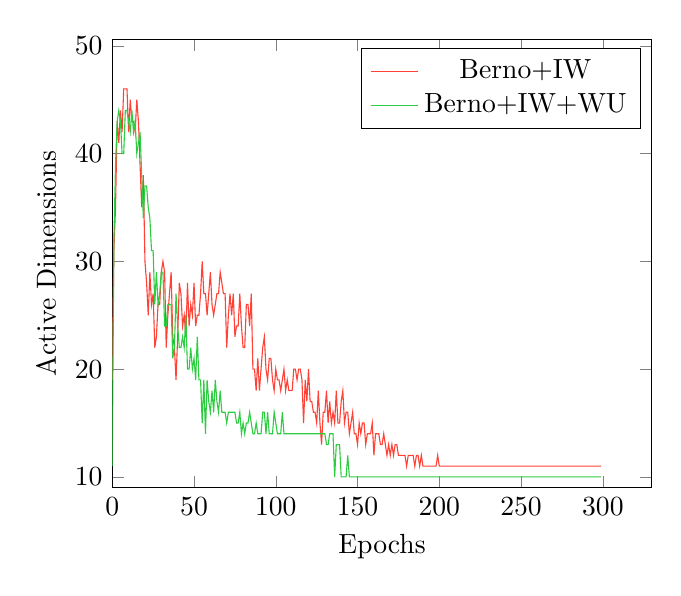
\begin{tikzpicture}\begin{axis}    [% title={Comparison of Importance Weighted and Warmed-Up for Activity},
    xlabel={Epochs},ylabel={Active Dimensions},    xmin=0.0, xmax=330.0,ymin=9.0, ymax=50.6,]    \addplot[color=red,]    coordinates {(0,19.0)(1,31.0)(2,35.0)(3,43.0)(4,41.0)(5,44.0)(6,42.0)(7,46.0)(8,46.0)(9,46.0)(10,42.0)(11,45.0)(12,43.0)(13,43.0)(14,42.0)(15,45.0)(16,43.0)(17,39.0)(18,35.0)(19,38.0)(20,30.0)(21,28.0)(22,25.0)(23,29.0)(24,26.0)(25,27.0)(26,22.0)(27,23.0)(28,26.0)(29,26.0)(30,29.0)(31,30.0)(32,29.0)(33,22.0)(34,25.0)(35,27.0)(36,29.0)(37,23.0)(38,22.0)(39,19.0)(40,23.0)(41,28.0)(42,27.0)(43,24.0)(44,25.0)(45,23.0)(46,28.0)(47,24.0)(48,26.0)(49,25.0)(50,28.0)(51,24.0)(52,25.0)(53,25.0)(54,27.0)(55,30.0)(56,27.0)(57,27.0)(58,25.0)(59,27.0)(60,29.0)(61,26.0)(62,25.0)(63,26.0)(64,27.0)(65,27.0)(66,29.0)(67,28.0)(68,27.0)(69,27.0)(70,22.0)(71,25.0)(72,27.0)(73,25.0)(74,27.0)(75,23.0)(76,24.0)(77,24.0)(78,27.0)(79,24.0)(80,22.0)(81,22.0)(82,26.0)(83,26.0)(84,24.0)(85,27.0)(86,20.0)(87,20.0)(88,18.0)(89,21.0)(90,18.0)(91,20.0)(92,22.0)(93,23.0)(94,20.0)(95,19.0)(96,21.0)(97,21.0)(98,19.0)(99,18.0)(100,20.0)(101,19.0)(102,19.0)(103,18.0)(104,19.0)(105,20.0)(106,18.0)(107,19.0)(108,18.0)(109,18.0)(110,18.0)(111,20.0)(112,20.0)(113,19.0)(114,20.0)(115,20.0)(116,19.0)(117,15.0)(118,19.0)(119,17.0)(120,20.0)(121,17.0)(122,17.0)(123,16.0)(124,16.0)(125,15.0)(126,18.0)(127,15.0)(128,13.0)(129,16.0)(130,16.0)(131,18.0)(132,15.0)(133,17.0)(134,15.0)(135,16.0)(136,15.0)(137,18.0)(138,15.0)(139,15.0)(140,17.0)(141,18.0)(142,15.0)(143,16.0)(144,16.0)(145,14.0)(146,15.0)(147,16.0)(148,14.0)(149,14.0)(150,13.0)(151,15.0)(152,14.0)(153,15.0)(154,15.0)(155,13.0)(156,14.0)(157,14.0)(158,14.0)(159,15.0)(160,12.0)(161,14.0)(162,14.0)(163,14.0)(164,13.0)(165,13.0)(166,14.0)(167,13.0)(168,12.0)(169,13.0)(170,12.0)(171,13.0)(172,12.0)(173,13.0)(174,13.0)(175,12.0)(176,12.0)(177,12.0)(178,12.0)(179,12.0)(180,11.0)(181,12.0)(182,12.0)(183,12.0)(184,12.0)(185,11.0)(186,12.0)(187,12.0)(188,11.0)(189,12.0)(190,11.0)(191,11.0)(192,11.0)(193,11.0)(194,11.0)(195,11.0)(196,11.0)(197,11.0)(198,11.0)(199,12.0)(200,11.0)(201,11.0)(202,11.0)(203,11.0)(204,11.0)(205,11.0)(206,11.0)(207,11.0)(208,11.0)(209,11.0)(210,11.0)(211,11.0)(212,11.0)(213,11.0)(214,11.0)(215,11.0)(216,11.0)(217,11.0)(218,11.0)(219,11.0)(220,11.0)(221,11.0)(222,11.0)(223,11.0)(224,11.0)(225,11.0)(226,11.0)(227,11.0)(228,11.0)(229,11.0)(230,11.0)(231,11.0)(232,11.0)(233,11.0)(234,11.0)(235,11.0)(236,11.0)(237,11.0)(238,11.0)(239,11.0)(240,11.0)(241,11.0)(242,11.0)(243,11.0)(244,11.0)(245,11.0)(246,11.0)(247,11.0)(248,11.0)(249,11.0)(250,11.0)(251,11.0)(252,11.0)(253,11.0)(254,11.0)(255,11.0)(256,11.0)(257,11.0)(258,11.0)(259,11.0)(260,11.0)(261,11.0)(262,11.0)(263,11.0)(264,11.0)(265,11.0)(266,11.0)(267,11.0)(268,11.0)(269,11.0)(270,11.0)(271,11.0)(272,11.0)(273,11.0)(274,11.0)(275,11.0)(276,11.0)(277,11.0)(278,11.0)(279,11.0)(280,11.0)(281,11.0)(282,11.0)(283,11.0)(284,11.0)(285,11.0)(286,11.0)(287,11.0)(288,11.0)(289,11.0)(290,11.0)(291,11.0)(292,11.0)(293,11.0)(294,11.0)(295,11.0)(296,11.0)(297,11.0)(298,11.0)(299,11.0)    };    \addplot[color=green,]    coordinates {(0,11.0)(1,32.0)(2,39.0)(3,43.0)(4,44.0)(5,43.0)(6,40.0)(7,40.0)(8,44.0)(9,44.0)(10,43.0)(11,42.0)(12,44.0)(13,42.0)(14,43.0)(15,40.0)(16,41.0)(17,42.0)(18,38.0)(19,34.0)(20,37.0)(21,37.0)(22,35.0)(23,34.0)(24,31.0)(25,31.0)(26,26.0)(27,29.0)(28,26.0)(29,27.0)(30,29.0)(31,29.0)(32,24.0)(33,24.0)(34,26.0)(35,26.0)(36,26.0)(37,21.0)(38,22.0)(39,27.0)(40,24.0)(41,22.0)(42,22.0)(43,23.0)(44,22.0)(45,25.0)(46,20.0)(47,20.0)(48,22.0)(49,20.0)(50,21.0)(51,19.0)(52,23.0)(53,19.0)(54,19.0)(55,15.0)(56,19.0)(57,14.0)(58,19.0)(59,17.0)(60,16.0)(61,18.0)(62,16.0)(63,19.0)(64,17.0)(65,16.0)(66,18.0)(67,16.0)(68,16.0)(69,16.0)(70,15.0)(71,16.0)(72,16.0)(73,16.0)(74,16.0)(75,16.0)(76,15.0)(77,15.0)(78,16.0)(79,14.0)(80,15.0)(81,14.0)(82,15.0)(83,15.0)(84,16.0)(85,15.0)(86,14.0)(87,14.0)(88,15.0)(89,14.0)(90,14.0)(91,14.0)(92,16.0)(93,16.0)(94,14.0)(95,16.0)(96,14.0)(97,14.0)(98,14.0)(99,16.0)(100,15.0)(101,14.0)(102,14.0)(103,14.0)(104,16.0)(105,14.0)(106,14.0)(107,14.0)(108,14.0)(109,14.0)(110,14.0)(111,14.0)(112,14.0)(113,14.0)(114,14.0)(115,14.0)(116,14.0)(117,14.0)(118,14.0)(119,14.0)(120,14.0)(121,14.0)(122,14.0)(123,14.0)(124,14.0)(125,14.0)(126,14.0)(127,14.0)(128,14.0)(129,14.0)(130,14.0)(131,13.0)(132,13.0)(133,14.0)(134,14.0)(135,14.0)(136,10.0)(137,13.0)(138,13.0)(139,13.0)(140,10.0)(141,10.0)(142,10.0)(143,10.0)(144,12.0)(145,10.0)(146,10.0)(147,10.0)(148,10.0)(149,10.0)(150,10.0)(151,10.0)(152,10.0)(153,10.0)(154,10.0)(155,10.0)(156,10.0)(157,10.0)(158,10.0)(159,10.0)(160,10.0)(161,10.0)(162,10.0)(163,10.0)(164,10.0)(165,10.0)(166,10.0)(167,10.0)(168,10.0)(169,10.0)(170,10.0)(171,10.0)(172,10.0)(173,10.0)(174,10.0)(175,10.0)(176,10.0)(177,10.0)(178,10.0)(179,10.0)(180,10.0)(181,10.0)(182,10.0)(183,10.0)(184,10.0)(185,10.0)(186,10.0)(187,10.0)(188,10.0)(189,10.0)(190,10.0)(191,10.0)(192,10.0)(193,10.0)(194,10.0)(195,10.0)(196,10.0)(197,10.0)(198,10.0)(199,10.0)(200,10.0)(201,10.0)(202,10.0)(203,10.0)(204,10.0)(205,10.0)(206,10.0)(207,10.0)(208,10.0)(209,10.0)(210,10.0)(211,10.0)(212,10.0)(213,10.0)(214,10.0)(215,10.0)(216,10.0)(217,10.0)(218,10.0)(219,10.0)(220,10.0)(221,10.0)(222,10.0)(223,10.0)(224,10.0)(225,10.0)(226,10.0)(227,10.0)(228,10.0)(229,10.0)(230,10.0)(231,10.0)(232,10.0)(233,10.0)(234,10.0)(235,10.0)(236,10.0)(237,10.0)(238,10.0)(239,10.0)(240,10.0)(241,10.0)(242,10.0)(243,10.0)(244,10.0)(245,10.0)(246,10.0)(247,10.0)(248,10.0)(249,10.0)(250,10.0)(251,10.0)(252,10.0)(253,10.0)(254,10.0)(255,10.0)(256,10.0)(257,10.0)(258,10.0)(259,10.0)(260,10.0)(261,10.0)(262,10.0)(263,10.0)(264,10.0)(265,10.0)(266,10.0)(267,10.0)(268,10.0)(269,10.0)(270,10.0)(271,10.0)(272,10.0)(273,10.0)(274,10.0)(275,10.0)(276,10.0)(277,10.0)(278,10.0)(279,10.0)(280,10.0)(281,10.0)(282,10.0)(283,10.0)(284,10.0)(285,10.0)(286,10.0)(287,10.0)(288,10.0)(289,10.0)(290,10.0)(291,10.0)(292,10.0)(293,10.0)(294,10.0)(295,10.0)(296,10.0)(297,10.0)(298,10.0)(299,10.0)    };    \legend{Berno+IW,Berno+IW+WU,}\end{axis}\end{tikzpicture}\\}
    \caption{Warm-Up}
    \label{fig:wulat}
  \end{subfigure}
  \caption{Effect of Methods on Latent Dimension Activity}
  \label{fig:activities}
\end{figure}
\subsection{Effects of Methods on Activity}
We observe from our experiments that the vanilla VAE tends to quickly prune latent dimensions, and once inactive those dimensions are not likely to reactivate. The effect of importance weighting seems to smooth the early pruning, as seen in Figure \ref{fig:iwlat}. We also note that importance weighting encourages convergence to fewer latent dimensions than the vanilla VAE. Batch normalization also reduced the rating of early pruning, but conversely encouraged convergence to a greater number of active latent dimensions. Interestingly, this behaviour is suggested as desirable for deep VAEs where increased latent activity is required for training of deeper layers. However, we know from previous results that the batch normalization does not improve training for our shallow VAEs. It is possible that by encouraging more active latent dimensions here, batch normalization may be reducing the effectiveness of the model to learn fewer, more representative dimensions. Finally, we see that warm-up also smooths early pruning over the importance weighted VAE, removing that drastic initial drop in active dimensions. It is interesting to note the pruning of latent dimensions continues smoothly throughout the entire warm-up period of 100 epochs. The number of active dimensions at the end of the warm-up period is near to the final converged value of dimensions. The converged value of active dimensions did not differ with warm-up from the importance weighted VAE.\\
It is interesting to note that with these methods the latent dimensionality tended to converge to $\sim 10$ active dimensions. This result further supports our previous observation that those additional latent dimensions become superfluous to learning. To explore this further we trained multiple VAEs with latent dimension $n_z \in \{2,5,10,20,50,100\}$ and observed the dimensional activity throughout training, see Figure \ref{fig:latdimlat}. Here we see that latent dimensions fewer than 10 were never pruned by training. All models with latent dimensionality greater than 10 had their active dimensions pruned to $\sim 10$ active dimensions. This suggests to us that the true posterior distribution for our dataset is best represented by a $\sim 10$-dimensional latent space. 
 
%It is clear from our experiments that, as training progresses, importance weighting tends to reduce the number of active dimensions, while batch normalization increases it. Warmup was not seen to affect the final dimensionality count, but did accelerate its convergence. The dimension-reducing effect of importance weighting is likely a result of its more accurate loss function, which reduces the capacity for error in the network and forces a more specific lower entropy latent representation of the data. The dimension-increasing effects of batch normalization are likely a result of its tendency to force a distribution on the output of the deterministic layers. This introduces noise in the form of an additional influence on the data that is passed to the latent layer, which it must then compensate for. The effect of warmup is likely a result of the distinct loss function, which punishes frivolous and incorrect information in the latent layer disproportionately in the early training stages.
%\par An interesting result can be seen in Figure \ref{fig:latdimlat}, in which the dimensionality is varied for models trained with importance weighting and neither batch normalization or warmup. As the dimensionality of the model increases, the number of active dimensions as the training converges tends to be constant at $min(D_{init},10)$ where $D_{init}$ is the number of dimensions being trained (the ``initial`` dimensionality of the latent space before pruning). This suggests that a fixed number of dimensions in the latent space may be ideal for representing a particular data set. In this case, 10. This is consistent with the results in Figure \ref{fig:latdimcost}, which indicated that an increase in the dimensionality beyond 10 had little effect on the loss function of the trained model.
\begin{wrapfigure}{l}{0.5\textwidth}
  \resizebox{\linewidth}{!}{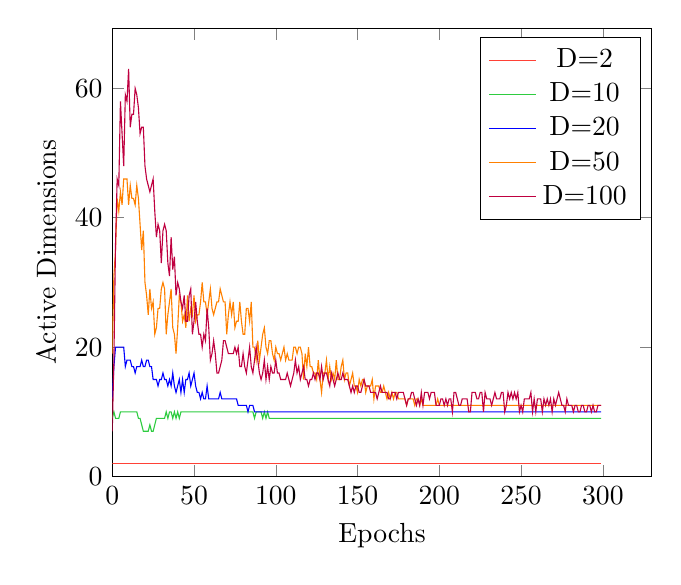
\begin{tikzpicture}\begin{axis}    [% title={Comparison of Dimension Values for Activity},
    xlabel={Epochs},ylabel={Active Dimensions},    xmin=0, xmax=330.0,ymin=0, ymax=69.3,]    \addplot[color=red,]    coordinates {(0,2.0)(1,2.0)(2,2.0)(3,2.0)(4,2.0)(5,2.0)(6,2.0)(7,2.0)(8,2.0)(9,2.0)(10,2.0)(11,2.0)(12,2.0)(13,2.0)(14,2.0)(15,2.0)(16,2.0)(17,2.0)(18,2.0)(19,2.0)(20,2.0)(21,2.0)(22,2.0)(23,2.0)(24,2.0)(25,2.0)(26,2.0)(27,2.0)(28,2.0)(29,2.0)(30,2.0)(31,2.0)(32,2.0)(33,2.0)(34,2.0)(35,2.0)(36,2.0)(37,2.0)(38,2.0)(39,2.0)(40,2.0)(41,2.0)(42,2.0)(43,2.0)(44,2.0)(45,2.0)(46,2.0)(47,2.0)(48,2.0)(49,2.0)(50,2.0)(51,2.0)(52,2.0)(53,2.0)(54,2.0)(55,2.0)(56,2.0)(57,2.0)(58,2.0)(59,2.0)(60,2.0)(61,2.0)(62,2.0)(63,2.0)(64,2.0)(65,2.0)(66,2.0)(67,2.0)(68,2.0)(69,2.0)(70,2.0)(71,2.0)(72,2.0)(73,2.0)(74,2.0)(75,2.0)(76,2.0)(77,2.0)(78,2.0)(79,2.0)(80,2.0)(81,2.0)(82,2.0)(83,2.0)(84,2.0)(85,2.0)(86,2.0)(87,2.0)(88,2.0)(89,2.0)(90,2.0)(91,2.0)(92,2.0)(93,2.0)(94,2.0)(95,2.0)(96,2.0)(97,2.0)(98,2.0)(99,2.0)(100,2.0)(101,2.0)(102,2.0)(103,2.0)(104,2.0)(105,2.0)(106,2.0)(107,2.0)(108,2.0)(109,2.0)(110,2.0)(111,2.0)(112,2.0)(113,2.0)(114,2.0)(115,2.0)(116,2.0)(117,2.0)(118,2.0)(119,2.0)(120,2.0)(121,2.0)(122,2.0)(123,2.0)(124,2.0)(125,2.0)(126,2.0)(127,2.0)(128,2.0)(129,2.0)(130,2.0)(131,2.0)(132,2.0)(133,2.0)(134,2.0)(135,2.0)(136,2.0)(137,2.0)(138,2.0)(139,2.0)(140,2.0)(141,2.0)(142,2.0)(143,2.0)(144,2.0)(145,2.0)(146,2.0)(147,2.0)(148,2.0)(149,2.0)(150,2.0)(151,2.0)(152,2.0)(153,2.0)(154,2.0)(155,2.0)(156,2.0)(157,2.0)(158,2.0)(159,2.0)(160,2.0)(161,2.0)(162,2.0)(163,2.0)(164,2.0)(165,2.0)(166,2.0)(167,2.0)(168,2.0)(169,2.0)(170,2.0)(171,2.0)(172,2.0)(173,2.0)(174,2.0)(175,2.0)(176,2.0)(177,2.0)(178,2.0)(179,2.0)(180,2.0)(181,2.0)(182,2.0)(183,2.0)(184,2.0)(185,2.0)(186,2.0)(187,2.0)(188,2.0)(189,2.0)(190,2.0)(191,2.0)(192,2.0)(193,2.0)(194,2.0)(195,2.0)(196,2.0)(197,2.0)(198,2.0)(199,2.0)(200,2.0)(201,2.0)(202,2.0)(203,2.0)(204,2.0)(205,2.0)(206,2.0)(207,2.0)(208,2.0)(209,2.0)(210,2.0)(211,2.0)(212,2.0)(213,2.0)(214,2.0)(215,2.0)(216,2.0)(217,2.0)(218,2.0)(219,2.0)(220,2.0)(221,2.0)(222,2.0)(223,2.0)(224,2.0)(225,2.0)(226,2.0)(227,2.0)(228,2.0)(229,2.0)(230,2.0)(231,2.0)(232,2.0)(233,2.0)(234,2.0)(235,2.0)(236,2.0)(237,2.0)(238,2.0)(239,2.0)(240,2.0)(241,2.0)(242,2.0)(243,2.0)(244,2.0)(245,2.0)(246,2.0)(247,2.0)(248,2.0)(249,2.0)(250,2.0)(251,2.0)(252,2.0)(253,2.0)(254,2.0)(255,2.0)(256,2.0)(257,2.0)(258,2.0)(259,2.0)(260,2.0)(261,2.0)(262,2.0)(263,2.0)(264,2.0)(265,2.0)(266,2.0)(267,2.0)(268,2.0)(269,2.0)(270,2.0)(271,2.0)(272,2.0)(273,2.0)(274,2.0)(275,2.0)(276,2.0)(277,2.0)(278,2.0)(279,2.0)(280,2.0)(281,2.0)(282,2.0)(283,2.0)(284,2.0)(285,2.0)(286,2.0)(287,2.0)(288,2.0)(289,2.0)(290,2.0)(291,2.0)(292,2.0)(293,2.0)(294,2.0)(295,2.0)(296,2.0)(297,2.0)(298,2.0)(299,2.0)    };    \addplot[color=green,]    coordinates {(0,9.0)(1,10.0)(2,9.0)(3,9.0)(4,9.0)(5,10.0)(6,10.0)(7,10.0)(8,10.0)(9,10.0)(10,10.0)(11,10.0)(12,10.0)(13,10.0)(14,10.0)(15,10.0)(16,9.0)(17,9.0)(18,8.0)(19,7.0)(20,7.0)(21,7.0)(22,7.0)(23,8.0)(24,7.0)(25,7.0)(26,8.0)(27,9.0)(28,9.0)(29,9.0)(30,9.0)(31,9.0)(32,9.0)(33,10.0)(34,9.0)(35,10.0)(36,10.0)(37,9.0)(38,10.0)(39,9.0)(40,10.0)(41,9.0)(42,10.0)(43,10.0)(44,10.0)(45,10.0)(46,10.0)(47,10.0)(48,10.0)(49,10.0)(50,10.0)(51,10.0)(52,10.0)(53,10.0)(54,10.0)(55,10.0)(56,10.0)(57,10.0)(58,10.0)(59,10.0)(60,10.0)(61,10.0)(62,10.0)(63,10.0)(64,10.0)(65,10.0)(66,10.0)(67,10.0)(68,10.0)(69,10.0)(70,10.0)(71,10.0)(72,10.0)(73,10.0)(74,10.0)(75,10.0)(76,10.0)(77,10.0)(78,10.0)(79,10.0)(80,10.0)(81,10.0)(82,10.0)(83,10.0)(84,10.0)(85,10.0)(86,10.0)(87,9.0)(88,10.0)(89,10.0)(90,10.0)(91,10.0)(92,9.0)(93,10.0)(94,9.0)(95,10.0)(96,9.0)(97,9.0)(98,9.0)(99,9.0)(100,9.0)(101,9.0)(102,9.0)(103,9.0)(104,9.0)(105,9.0)(106,9.0)(107,9.0)(108,9.0)(109,9.0)(110,9.0)(111,9.0)(112,9.0)(113,9.0)(114,9.0)(115,9.0)(116,9.0)(117,9.0)(118,9.0)(119,9.0)(120,9.0)(121,9.0)(122,9.0)(123,9.0)(124,9.0)(125,9.0)(126,9.0)(127,9.0)(128,9.0)(129,9.0)(130,9.0)(131,9.0)(132,9.0)(133,9.0)(134,9.0)(135,9.0)(136,9.0)(137,9.0)(138,9.0)(139,9.0)(140,9.0)(141,9.0)(142,9.0)(143,9.0)(144,9.0)(145,9.0)(146,9.0)(147,9.0)(148,9.0)(149,9.0)(150,9.0)(151,9.0)(152,9.0)(153,9.0)(154,9.0)(155,9.0)(156,9.0)(157,9.0)(158,9.0)(159,9.0)(160,9.0)(161,9.0)(162,9.0)(163,9.0)(164,9.0)(165,9.0)(166,9.0)(167,9.0)(168,9.0)(169,9.0)(170,9.0)(171,9.0)(172,9.0)(173,9.0)(174,9.0)(175,9.0)(176,9.0)(177,9.0)(178,9.0)(179,9.0)(180,9.0)(181,9.0)(182,9.0)(183,9.0)(184,9.0)(185,9.0)(186,9.0)(187,9.0)(188,9.0)(189,9.0)(190,9.0)(191,9.0)(192,9.0)(193,9.0)(194,9.0)(195,9.0)(196,9.0)(197,9.0)(198,9.0)(199,9.0)(200,9.0)(201,9.0)(202,9.0)(203,9.0)(204,9.0)(205,9.0)(206,9.0)(207,9.0)(208,9.0)(209,9.0)(210,9.0)(211,9.0)(212,9.0)(213,9.0)(214,9.0)(215,9.0)(216,9.0)(217,9.0)(218,9.0)(219,9.0)(220,9.0)(221,9.0)(222,9.0)(223,9.0)(224,9.0)(225,9.0)(226,9.0)(227,9.0)(228,9.0)(229,9.0)(230,9.0)(231,9.0)(232,9.0)(233,9.0)(234,9.0)(235,9.0)(236,9.0)(237,9.0)(238,9.0)(239,9.0)(240,9.0)(241,9.0)(242,9.0)(243,9.0)(244,9.0)(245,9.0)(246,9.0)(247,9.0)(248,9.0)(249,9.0)(250,9.0)(251,9.0)(252,9.0)(253,9.0)(254,9.0)(255,9.0)(256,9.0)(257,9.0)(258,9.0)(259,9.0)(260,9.0)(261,9.0)(262,9.0)(263,9.0)(264,9.0)(265,9.0)(266,9.0)(267,9.0)(268,9.0)(269,9.0)(270,9.0)(271,9.0)(272,9.0)(273,9.0)(274,9.0)(275,9.0)(276,9.0)(277,9.0)(278,9.0)(279,9.0)(280,9.0)(281,9.0)(282,9.0)(283,9.0)(284,9.0)(285,9.0)(286,9.0)(287,9.0)(288,9.0)(289,9.0)(290,9.0)(291,9.0)(292,9.0)(293,9.0)(294,9.0)(295,9.0)(296,9.0)(297,9.0)(298,9.0)(299,9.0)    };    \addplot[color=blue,]    coordinates {(0,12.0)(1,17.0)(2,20.0)(3,20.0)(4,20.0)(5,20.0)(6,20.0)(7,20.0)(8,17.0)(9,18.0)(10,18.0)(11,18.0)(12,17.0)(13,17.0)(14,16.0)(15,17.0)(16,17.0)(17,17.0)(18,18.0)(19,17.0)(20,17.0)(21,18.0)(22,18.0)(23,17.0)(24,17.0)(25,15.0)(26,15.0)(27,15.0)(28,14.0)(29,15.0)(30,15.0)(31,16.0)(32,15.0)(33,15.0)(34,14.0)(35,15.0)(36,14.0)(37,16.0)(38,14.0)(39,13.0)(40,14.0)(41,15.0)(42,13.0)(43,15.0)(44,13.0)(45,15.0)(46,15.0)(47,16.0)(48,14.0)(49,15.0)(50,16.0)(51,14.0)(52,13.0)(53,13.0)(54,12.0)(55,13.0)(56,12.0)(57,12.0)(58,14.0)(59,12.0)(60,12.0)(61,12.0)(62,12.0)(63,12.0)(64,12.0)(65,12.0)(66,13.0)(67,12.0)(68,12.0)(69,12.0)(70,12.0)(71,12.0)(72,12.0)(73,12.0)(74,12.0)(75,12.0)(76,12.0)(77,11.0)(78,11.0)(79,11.0)(80,11.0)(81,11.0)(82,11.0)(83,10.0)(84,11.0)(85,11.0)(86,11.0)(87,10.0)(88,10.0)(89,10.0)(90,10.0)(91,10.0)(92,10.0)(93,10.0)(94,10.0)(95,10.0)(96,10.0)(97,10.0)(98,10.0)(99,10.0)(100,10.0)(101,10.0)(102,10.0)(103,10.0)(104,10.0)(105,10.0)(106,10.0)(107,10.0)(108,10.0)(109,10.0)(110,10.0)(111,10.0)(112,10.0)(113,10.0)(114,10.0)(115,10.0)(116,10.0)(117,10.0)(118,10.0)(119,10.0)(120,10.0)(121,10.0)(122,10.0)(123,10.0)(124,10.0)(125,10.0)(126,10.0)(127,10.0)(128,10.0)(129,10.0)(130,10.0)(131,10.0)(132,10.0)(133,10.0)(134,10.0)(135,10.0)(136,10.0)(137,10.0)(138,10.0)(139,10.0)(140,10.0)(141,10.0)(142,10.0)(143,10.0)(144,10.0)(145,10.0)(146,10.0)(147,10.0)(148,10.0)(149,10.0)(150,10.0)(151,10.0)(152,10.0)(153,10.0)(154,10.0)(155,10.0)(156,10.0)(157,10.0)(158,10.0)(159,10.0)(160,10.0)(161,10.0)(162,10.0)(163,10.0)(164,10.0)(165,10.0)(166,10.0)(167,10.0)(168,10.0)(169,10.0)(170,10.0)(171,10.0)(172,10.0)(173,10.0)(174,10.0)(175,10.0)(176,10.0)(177,10.0)(178,10.0)(179,10.0)(180,10.0)(181,10.0)(182,10.0)(183,10.0)(184,10.0)(185,10.0)(186,10.0)(187,10.0)(188,10.0)(189,10.0)(190,10.0)(191,10.0)(192,10.0)(193,10.0)(194,10.0)(195,10.0)(196,10.0)(197,10.0)(198,10.0)(199,10.0)(200,10.0)(201,10.0)(202,10.0)(203,10.0)(204,10.0)(205,10.0)(206,10.0)(207,10.0)(208,10.0)(209,10.0)(210,10.0)(211,10.0)(212,10.0)(213,10.0)(214,10.0)(215,10.0)(216,10.0)(217,10.0)(218,10.0)(219,10.0)(220,10.0)(221,10.0)(222,10.0)(223,10.0)(224,10.0)(225,10.0)(226,10.0)(227,10.0)(228,10.0)(229,10.0)(230,10.0)(231,10.0)(232,10.0)(233,10.0)(234,10.0)(235,10.0)(236,10.0)(237,10.0)(238,10.0)(239,10.0)(240,10.0)(241,10.0)(242,10.0)(243,10.0)(244,10.0)(245,10.0)(246,10.0)(247,10.0)(248,10.0)(249,10.0)(250,10.0)(251,10.0)(252,10.0)(253,10.0)(254,10.0)(255,10.0)(256,10.0)(257,10.0)(258,10.0)(259,10.0)(260,10.0)(261,10.0)(262,10.0)(263,10.0)(264,10.0)(265,10.0)(266,10.0)(267,10.0)(268,10.0)(269,10.0)(270,10.0)(271,10.0)(272,10.0)(273,10.0)(274,10.0)(275,10.0)(276,10.0)(277,10.0)(278,10.0)(279,10.0)(280,10.0)(281,10.0)(282,10.0)(283,10.0)(284,10.0)(285,10.0)(286,10.0)(287,10.0)(288,10.0)(289,10.0)(290,10.0)(291,10.0)(292,10.0)(293,10.0)(294,10.0)(295,10.0)(296,10.0)(297,10.0)(298,10.0)(299,10.0)    };    \addplot[color=orange,]    coordinates {(0,19.0)(1,31.0)(2,35.0)(3,43.0)(4,41.0)(5,44.0)(6,42.0)(7,46.0)(8,46.0)(9,46.0)(10,42.0)(11,45.0)(12,43.0)(13,43.0)(14,42.0)(15,45.0)(16,43.0)(17,39.0)(18,35.0)(19,38.0)(20,30.0)(21,28.0)(22,25.0)(23,29.0)(24,26.0)(25,27.0)(26,22.0)(27,23.0)(28,26.0)(29,26.0)(30,29.0)(31,30.0)(32,29.0)(33,22.0)(34,25.0)(35,27.0)(36,29.0)(37,23.0)(38,22.0)(39,19.0)(40,23.0)(41,28.0)(42,27.0)(43,24.0)(44,25.0)(45,23.0)(46,28.0)(47,24.0)(48,26.0)(49,25.0)(50,28.0)(51,24.0)(52,25.0)(53,25.0)(54,27.0)(55,30.0)(56,27.0)(57,27.0)(58,25.0)(59,27.0)(60,29.0)(61,26.0)(62,25.0)(63,26.0)(64,27.0)(65,27.0)(66,29.0)(67,28.0)(68,27.0)(69,27.0)(70,22.0)(71,25.0)(72,27.0)(73,25.0)(74,27.0)(75,23.0)(76,24.0)(77,24.0)(78,27.0)(79,24.0)(80,22.0)(81,22.0)(82,26.0)(83,26.0)(84,24.0)(85,27.0)(86,20.0)(87,20.0)(88,18.0)(89,21.0)(90,18.0)(91,20.0)(92,22.0)(93,23.0)(94,20.0)(95,19.0)(96,21.0)(97,21.0)(98,19.0)(99,18.0)(100,20.0)(101,19.0)(102,19.0)(103,18.0)(104,19.0)(105,20.0)(106,18.0)(107,19.0)(108,18.0)(109,18.0)(110,18.0)(111,20.0)(112,20.0)(113,19.0)(114,20.0)(115,20.0)(116,19.0)(117,15.0)(118,19.0)(119,17.0)(120,20.0)(121,17.0)(122,17.0)(123,16.0)(124,16.0)(125,15.0)(126,18.0)(127,15.0)(128,13.0)(129,16.0)(130,16.0)(131,18.0)(132,15.0)(133,17.0)(134,15.0)(135,16.0)(136,15.0)(137,18.0)(138,15.0)(139,15.0)(140,17.0)(141,18.0)(142,15.0)(143,16.0)(144,16.0)(145,14.0)(146,15.0)(147,16.0)(148,14.0)(149,14.0)(150,13.0)(151,15.0)(152,14.0)(153,15.0)(154,15.0)(155,13.0)(156,14.0)(157,14.0)(158,14.0)(159,15.0)(160,12.0)(161,14.0)(162,14.0)(163,14.0)(164,13.0)(165,13.0)(166,14.0)(167,13.0)(168,12.0)(169,13.0)(170,12.0)(171,13.0)(172,12.0)(173,13.0)(174,13.0)(175,12.0)(176,12.0)(177,12.0)(178,12.0)(179,12.0)(180,11.0)(181,12.0)(182,12.0)(183,12.0)(184,12.0)(185,11.0)(186,12.0)(187,12.0)(188,11.0)(189,12.0)(190,11.0)(191,11.0)(192,11.0)(193,11.0)(194,11.0)(195,11.0)(196,11.0)(197,11.0)(198,11.0)(199,12.0)(200,11.0)(201,11.0)(202,11.0)(203,11.0)(204,11.0)(205,11.0)(206,11.0)(207,11.0)(208,11.0)(209,11.0)(210,11.0)(211,11.0)(212,11.0)(213,11.0)(214,11.0)(215,11.0)(216,11.0)(217,11.0)(218,11.0)(219,11.0)(220,11.0)(221,11.0)(222,11.0)(223,11.0)(224,11.0)(225,11.0)(226,11.0)(227,11.0)(228,11.0)(229,11.0)(230,11.0)(231,11.0)(232,11.0)(233,11.0)(234,11.0)(235,11.0)(236,11.0)(237,11.0)(238,11.0)(239,11.0)(240,11.0)(241,11.0)(242,11.0)(243,11.0)(244,11.0)(245,11.0)(246,11.0)(247,11.0)(248,11.0)(249,11.0)(250,11.0)(251,11.0)(252,11.0)(253,11.0)(254,11.0)(255,11.0)(256,11.0)(257,11.0)(258,11.0)(259,11.0)(260,11.0)(261,11.0)(262,11.0)(263,11.0)(264,11.0)(265,11.0)(266,11.0)(267,11.0)(268,11.0)(269,11.0)(270,11.0)(271,11.0)(272,11.0)(273,11.0)(274,11.0)(275,11.0)(276,11.0)(277,11.0)(278,11.0)(279,11.0)(280,11.0)(281,11.0)(282,11.0)(283,11.0)(284,11.0)(285,11.0)(286,11.0)(287,11.0)(288,11.0)(289,11.0)(290,11.0)(291,11.0)(292,11.0)(293,11.0)(294,11.0)(295,11.0)(296,11.0)(297,11.0)(298,11.0)(299,11.0)    };    \addplot[color=purple,]    coordinates {(0,7.0)(1,18.0)(2,36.0)(3,46.0)(4,45.0)(5,58.0)(6,53.0)(7,48.0)(8,59.0)(9,58.0)(10,63.0)(11,54.0)(12,56.0)(13,56.0)(14,60.0)(15,59.0)(16,57.0)(17,53.0)(18,54.0)(19,54.0)(20,48.0)(21,46.0)(22,45.0)(23,44.0)(24,45.0)(25,46.0)(26,41.0)(27,37.0)(28,39.0)(29,38.0)(30,33.0)(31,38.0)(32,39.0)(33,38.0)(34,33.0)(35,31.0)(36,37.0)(37,32.0)(38,34.0)(39,28.0)(40,30.0)(41,29.0)(42,27.0)(43,26.0)(44,28.0)(45,24.0)(46,24.0)(47,28.0)(48,29.0)(49,22.0)(50,24.0)(51,27.0)(52,24.0)(53,22.0)(54,22.0)(55,20.0)(56,22.0)(57,21.0)(58,26.0)(59,23.0)(60,18.0)(61,19.0)(62,21.0)(63,19.0)(64,16.0)(65,16.0)(66,17.0)(67,18.0)(68,21.0)(69,21.0)(70,20.0)(71,19.0)(72,19.0)(73,19.0)(74,19.0)(75,20.0)(76,19.0)(77,20.0)(78,17.0)(79,17.0)(80,19.0)(81,17.0)(82,16.0)(83,18.0)(84,20.0)(85,17.0)(86,16.0)(87,18.0)(88,20.0)(89,18.0)(90,16.0)(91,15.0)(92,16.0)(93,18.0)(94,15.0)(95,17.0)(96,15.0)(97,17.0)(98,16.0)(99,16.0)(100,18.0)(101,16.0)(102,16.0)(103,15.0)(104,15.0)(105,15.0)(106,15.0)(107,16.0)(108,15.0)(109,14.0)(110,15.0)(111,16.0)(112,18.0)(113,16.0)(114,17.0)(115,15.0)(116,16.0)(117,17.0)(118,15.0)(119,15.0)(120,14.0)(121,15.0)(122,15.0)(123,16.0)(124,15.0)(125,16.0)(126,16.0)(127,15.0)(128,17.0)(129,15.0)(130,16.0)(131,16.0)(132,15.0)(133,14.0)(134,16.0)(135,15.0)(136,14.0)(137,15.0)(138,16.0)(139,15.0)(140,15.0)(141,16.0)(142,15.0)(143,15.0)(144,15.0)(145,14.0)(146,13.0)(147,14.0)(148,13.0)(149,14.0)(150,14.0)(151,13.0)(152,13.0)(153,14.0)(154,15.0)(155,14.0)(156,14.0)(157,14.0)(158,13.0)(159,13.0)(160,13.0)(161,13.0)(162,12.0)(163,13.0)(164,14.0)(165,13.0)(166,13.0)(167,13.0)(168,13.0)(169,12.0)(170,12.0)(171,13.0)(172,13.0)(173,13.0)(174,12.0)(175,13.0)(176,13.0)(177,13.0)(178,13.0)(179,12.0)(180,11.0)(181,12.0)(182,12.0)(183,13.0)(184,13.0)(185,12.0)(186,11.0)(187,12.0)(188,11.0)(189,13.0)(190,11.0)(191,13.0)(192,13.0)(193,13.0)(194,12.0)(195,13.0)(196,13.0)(197,13.0)(198,11.0)(199,11.0)(200,11.0)(201,12.0)(202,12.0)(203,11.0)(204,12.0)(205,11.0)(206,12.0)(207,12.0)(208,10.0)(209,13.0)(210,13.0)(211,12.0)(212,11.0)(213,11.0)(214,12.0)(215,12.0)(216,12.0)(217,12.0)(218,10.0)(219,10.0)(220,13.0)(221,13.0)(222,13.0)(223,12.0)(224,12.0)(225,13.0)(226,13.0)(227,10.0)(228,13.0)(229,12.0)(230,12.0)(231,12.0)(232,11.0)(233,12.0)(234,13.0)(235,12.0)(236,12.0)(237,12.0)(238,13.0)(239,13.0)(240,10.0)(241,11.0)(242,13.0)(243,12.0)(244,13.0)(245,12.0)(246,13.0)(247,12.0)(248,13.0)(249,10.0)(250,11.0)(251,10.0)(252,12.0)(253,12.0)(254,12.0)(255,12.0)(256,13.0)(257,10.0)(258,12.0)(259,10.0)(260,12.0)(261,12.0)(262,12.0)(263,10.0)(264,12.0)(265,11.0)(266,12.0)(267,11.0)(268,12.0)(269,10.0)(270,12.0)(271,11.0)(272,12.0)(273,13.0)(274,12.0)(275,11.0)(276,11.0)(277,10.0)(278,12.0)(279,11.0)(280,11.0)(281,11.0)(282,10.0)(283,11.0)(284,11.0)(285,10.0)(286,10.0)(287,11.0)(288,11.0)(289,10.0)(290,10.0)(291,11.0)(292,11.0)(293,10.0)(294,11.0)(295,10.0)(296,10.0)(297,11.0)(298,11.0)(299,11.0)    };    \legend{D=2,D=10,D=20,D=50,D=100,}\end{axis}\end{tikzpicture}\\}
  \caption{Effect of Latent Dimensionality}
  \label{fig:latdimlat}
\end{wrapfigure}
\subsection{Visualizing Latent Space Activity during Training}
In their research S{\o}nderby et al. \cite{Sonderby2016} put forward a shaded rectangle plot for latent space activation that we have adapted below in Figure \ref{fig:shadeall}. In these plots, the $x$-axis represents training epochs and the $y$-axis represents the index of a dimension, sorted for clarity by initial activity. The shade of a pixel at a each coordinate represents the log of the activation defined in \ref{eq:ACTIVITYMET} for each dimension and epoch. The log-activation is calculated by sampling the variance of the dimensional mean over a random subset of the data. These shade plots provide a more holistic view of the activity than simply plotting the number of dimensions whose activity exceeds the threshold. For examples, in Figures \ref{fig:shadeiw}, \ref{fig:shadebn}, and \ref{fig:shadewu} it is clear that the dimensions labelled as inactive by the threshold measurement are making a nonzero contribution to the output of the latent layer, which may be useful in deep VAEs, and based on the cost functions plotted in Figures \ref{fig:variw}and \ref{fig:wucost} may useful in improving the accuracy of the model.
\begin{figure}[h]
  \centering
  \begin{subfigure}[t]{0.45\textwidth}
    \resizebox{\linewidth}{!}{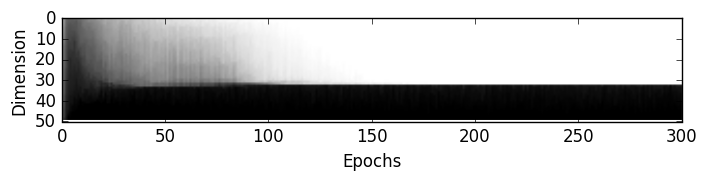
\includegraphics[scale=1]{{../plots/img/trial.50.1.0.0.0.0.Berno}.png}}
    \caption{Vanilla VAE with Bernoulli Decoder Distribution}
    \label{fig:shadevanil}    
  \end{subfigure}
  \begin{subfigure}[t]{0.45\textwidth}
    \resizebox{\linewidth}{!}{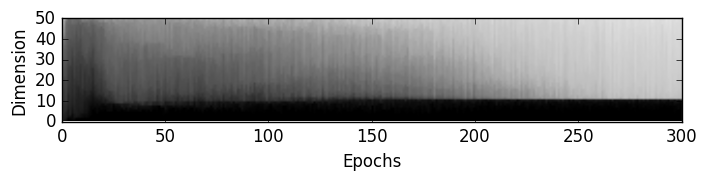
\includegraphics[scale=1]{{../plots/img/trial.50.1.0.0.0.1.Berno+IW}.png}}
    \caption{Importance Weighted (IW)}
    \label{fig:shadeiw}
  \end{subfigure}
  \begin{subfigure}[t]{0.45\textwidth}
    \resizebox{\linewidth}{!}{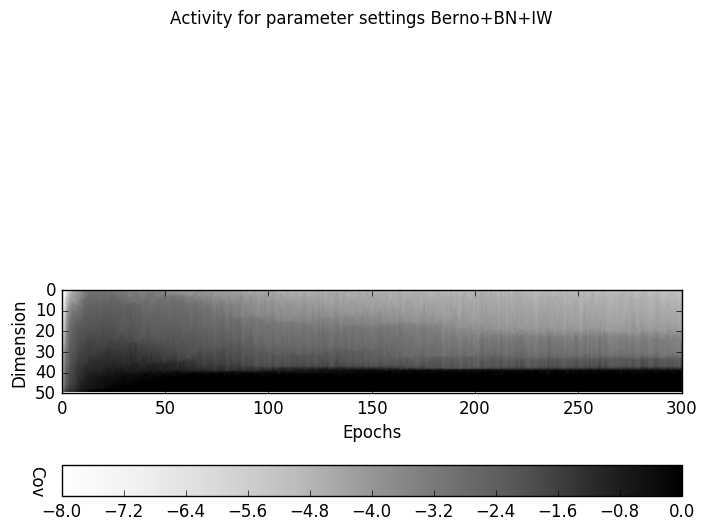
\includegraphics[scale=1]{{../plots/img/trial.50.1.0.1.0.1.Berno+BN+IW}.png}}
    \caption{IW + Batch Normalization (BN)}
    \label{fig:shadebn}
  \end{subfigure}
  \begin{subfigure}[t]{0.45\textwidth}
    \resizebox{\linewidth}{!}{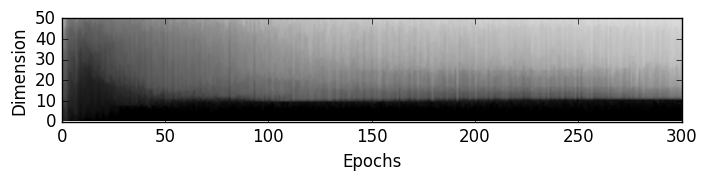
\includegraphics[scale=1]{{../plots/img/trial.50.1.0.0.1.1.Berno+WU+IW}.png}}
    \caption{IW + Warm Up (WU)}
    \label{fig:shadewu}
  \end{subfigure}
  \begin{subfigure}{0.8\textwidth}
    \resizebox{\linewidth}{!}{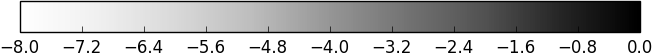
\includegraphics[scale=1]{{../plots/img/colorbar}.png}}
    \caption*{$\log{\left[Cov_{\textbf{x}}\left(\mathbb{E}_{u~q(u|\textbf{x})}[u]\right)\right]}$}
    \label{fig:shadebar}
  \end{subfigure}
  \caption{Latent Dimension Activity During Training}
  \label{fig:shadeall}
\end{figure}
\section{Latent Space Visualization}
\subsection{Data Reconstruction}
The first and most apparent technique for visualizing the model learned by our VAEs is to generate images of reconstructed input data. In this visualization we give a single test input to our VAE. The test input is first encoded to a representation in the latent space by the encoder network, then decoded to a reconstructed value in the data space. We generated examples of reconstruction visualizations for VAEs with 2 and 50 latent dimensions, see Figure \ref{fig:recon}. As expected, the 50 dimensional VAE was able to learn better representations of every test input than the 2 dimensional VAE. The 2 dimensional VAE performed comparably well on certain input classes, namely digits 1 and 7, but was completely unable to represent other classes, digits 2 and 0. To better understand why our 2 dimensional VAE was unable to learn representations for these classes, we utilize other visualization techniques which illustrate the distribution of the data classes in the latent space.
\subsection{Data Latent Encoding}
\begin{wrapfigure}{l}{0.5\textwidth}
    \resizebox{\linewidth}{!}{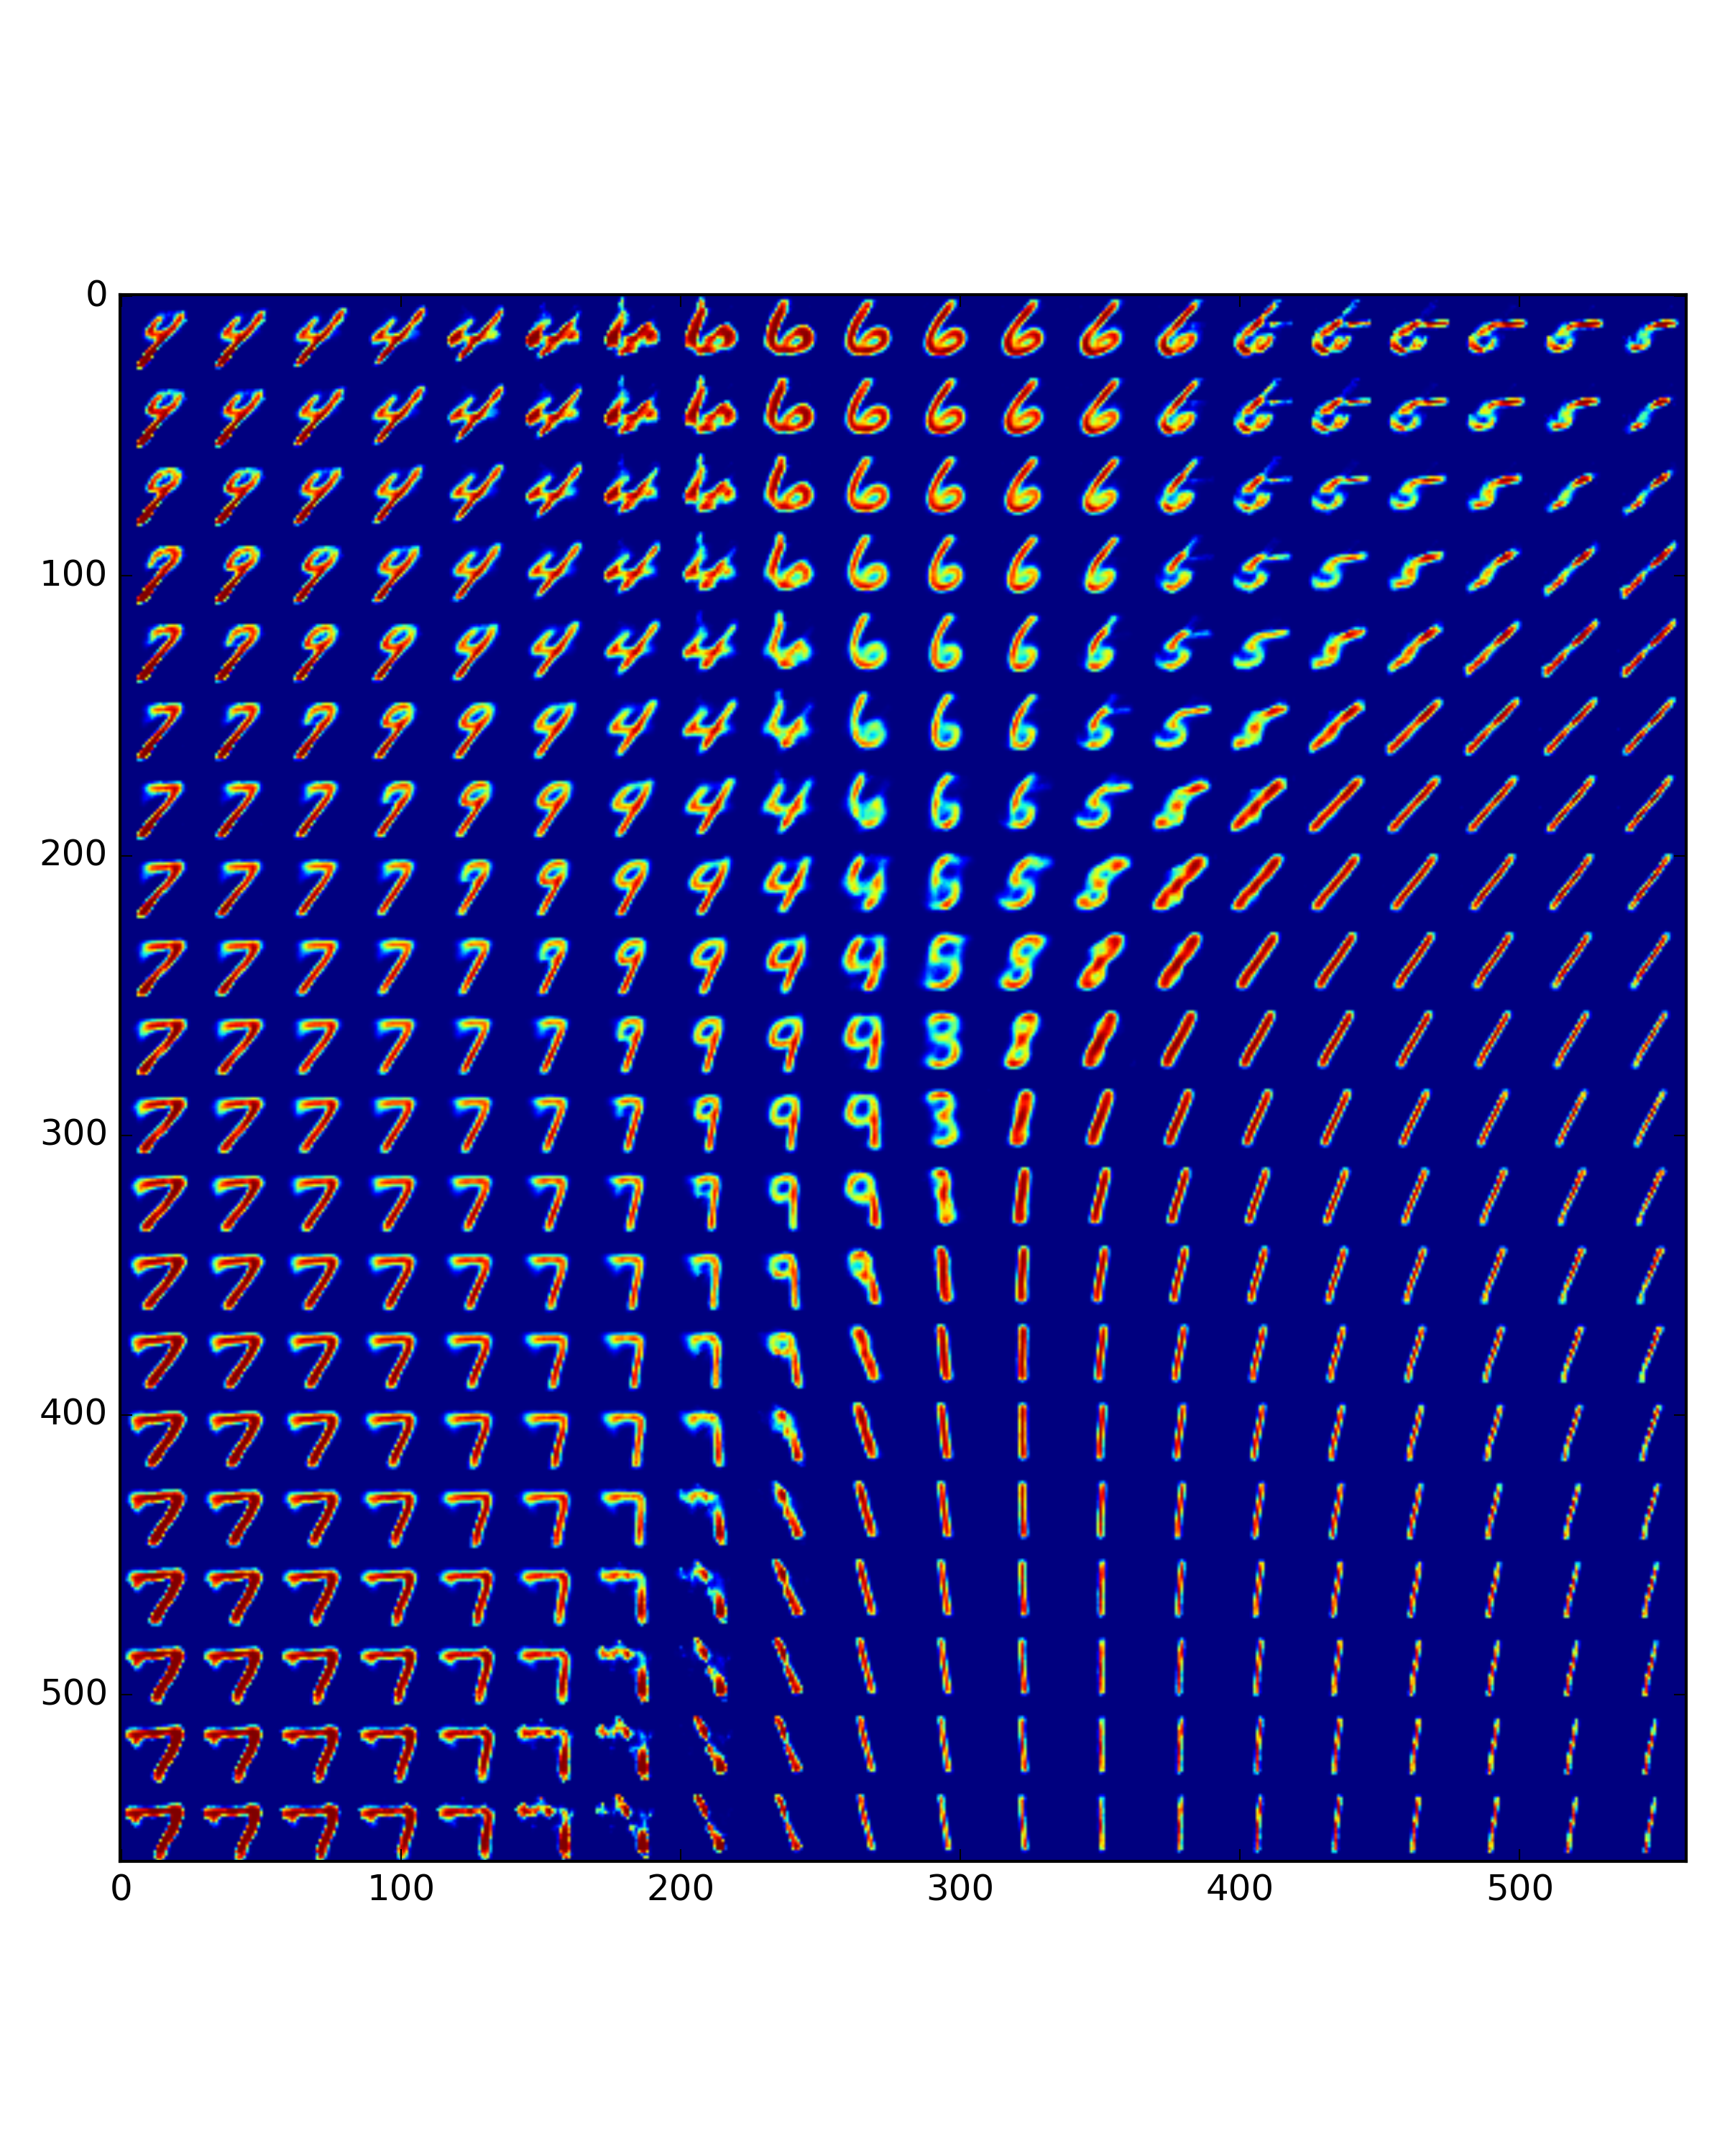
\includegraphics[scale=1]{{../plots/img/vis_latent2_1}.png}}
    \caption{Latent Manifold Visualization}
    \label{fig:latlattice}
\end{wrapfigure}
This visualization technique utilizes only the encoder network of our VAE. To understand how our data classes are encoded into the latent distribution, we input a subset of our data and plot their code values in latent space. For an example of this visualization with our 2 dimensional VAE, see Figure \ref{fig:latenc}. This visualization method clearly demonstrates which classes the VAE successfully modelled, and which classes were poorly represented. From our previous visualization, we observed that digits 1 and 7 were clearly reconstructed, and the data encoding visualization demonstrates why. Data classes which are clearly distinguished in latent space from other classes were better constructed by our VAE. Notice that the classes for digits 2 and 3 are not distinguished in the latent encoding, this corresponds to the incorrect reconstruction we observed previously.
\begin{figure}
  \centering
  \begin{minipage}[b]{0.45\textwidth}
    \resizebox{\linewidth}{!}{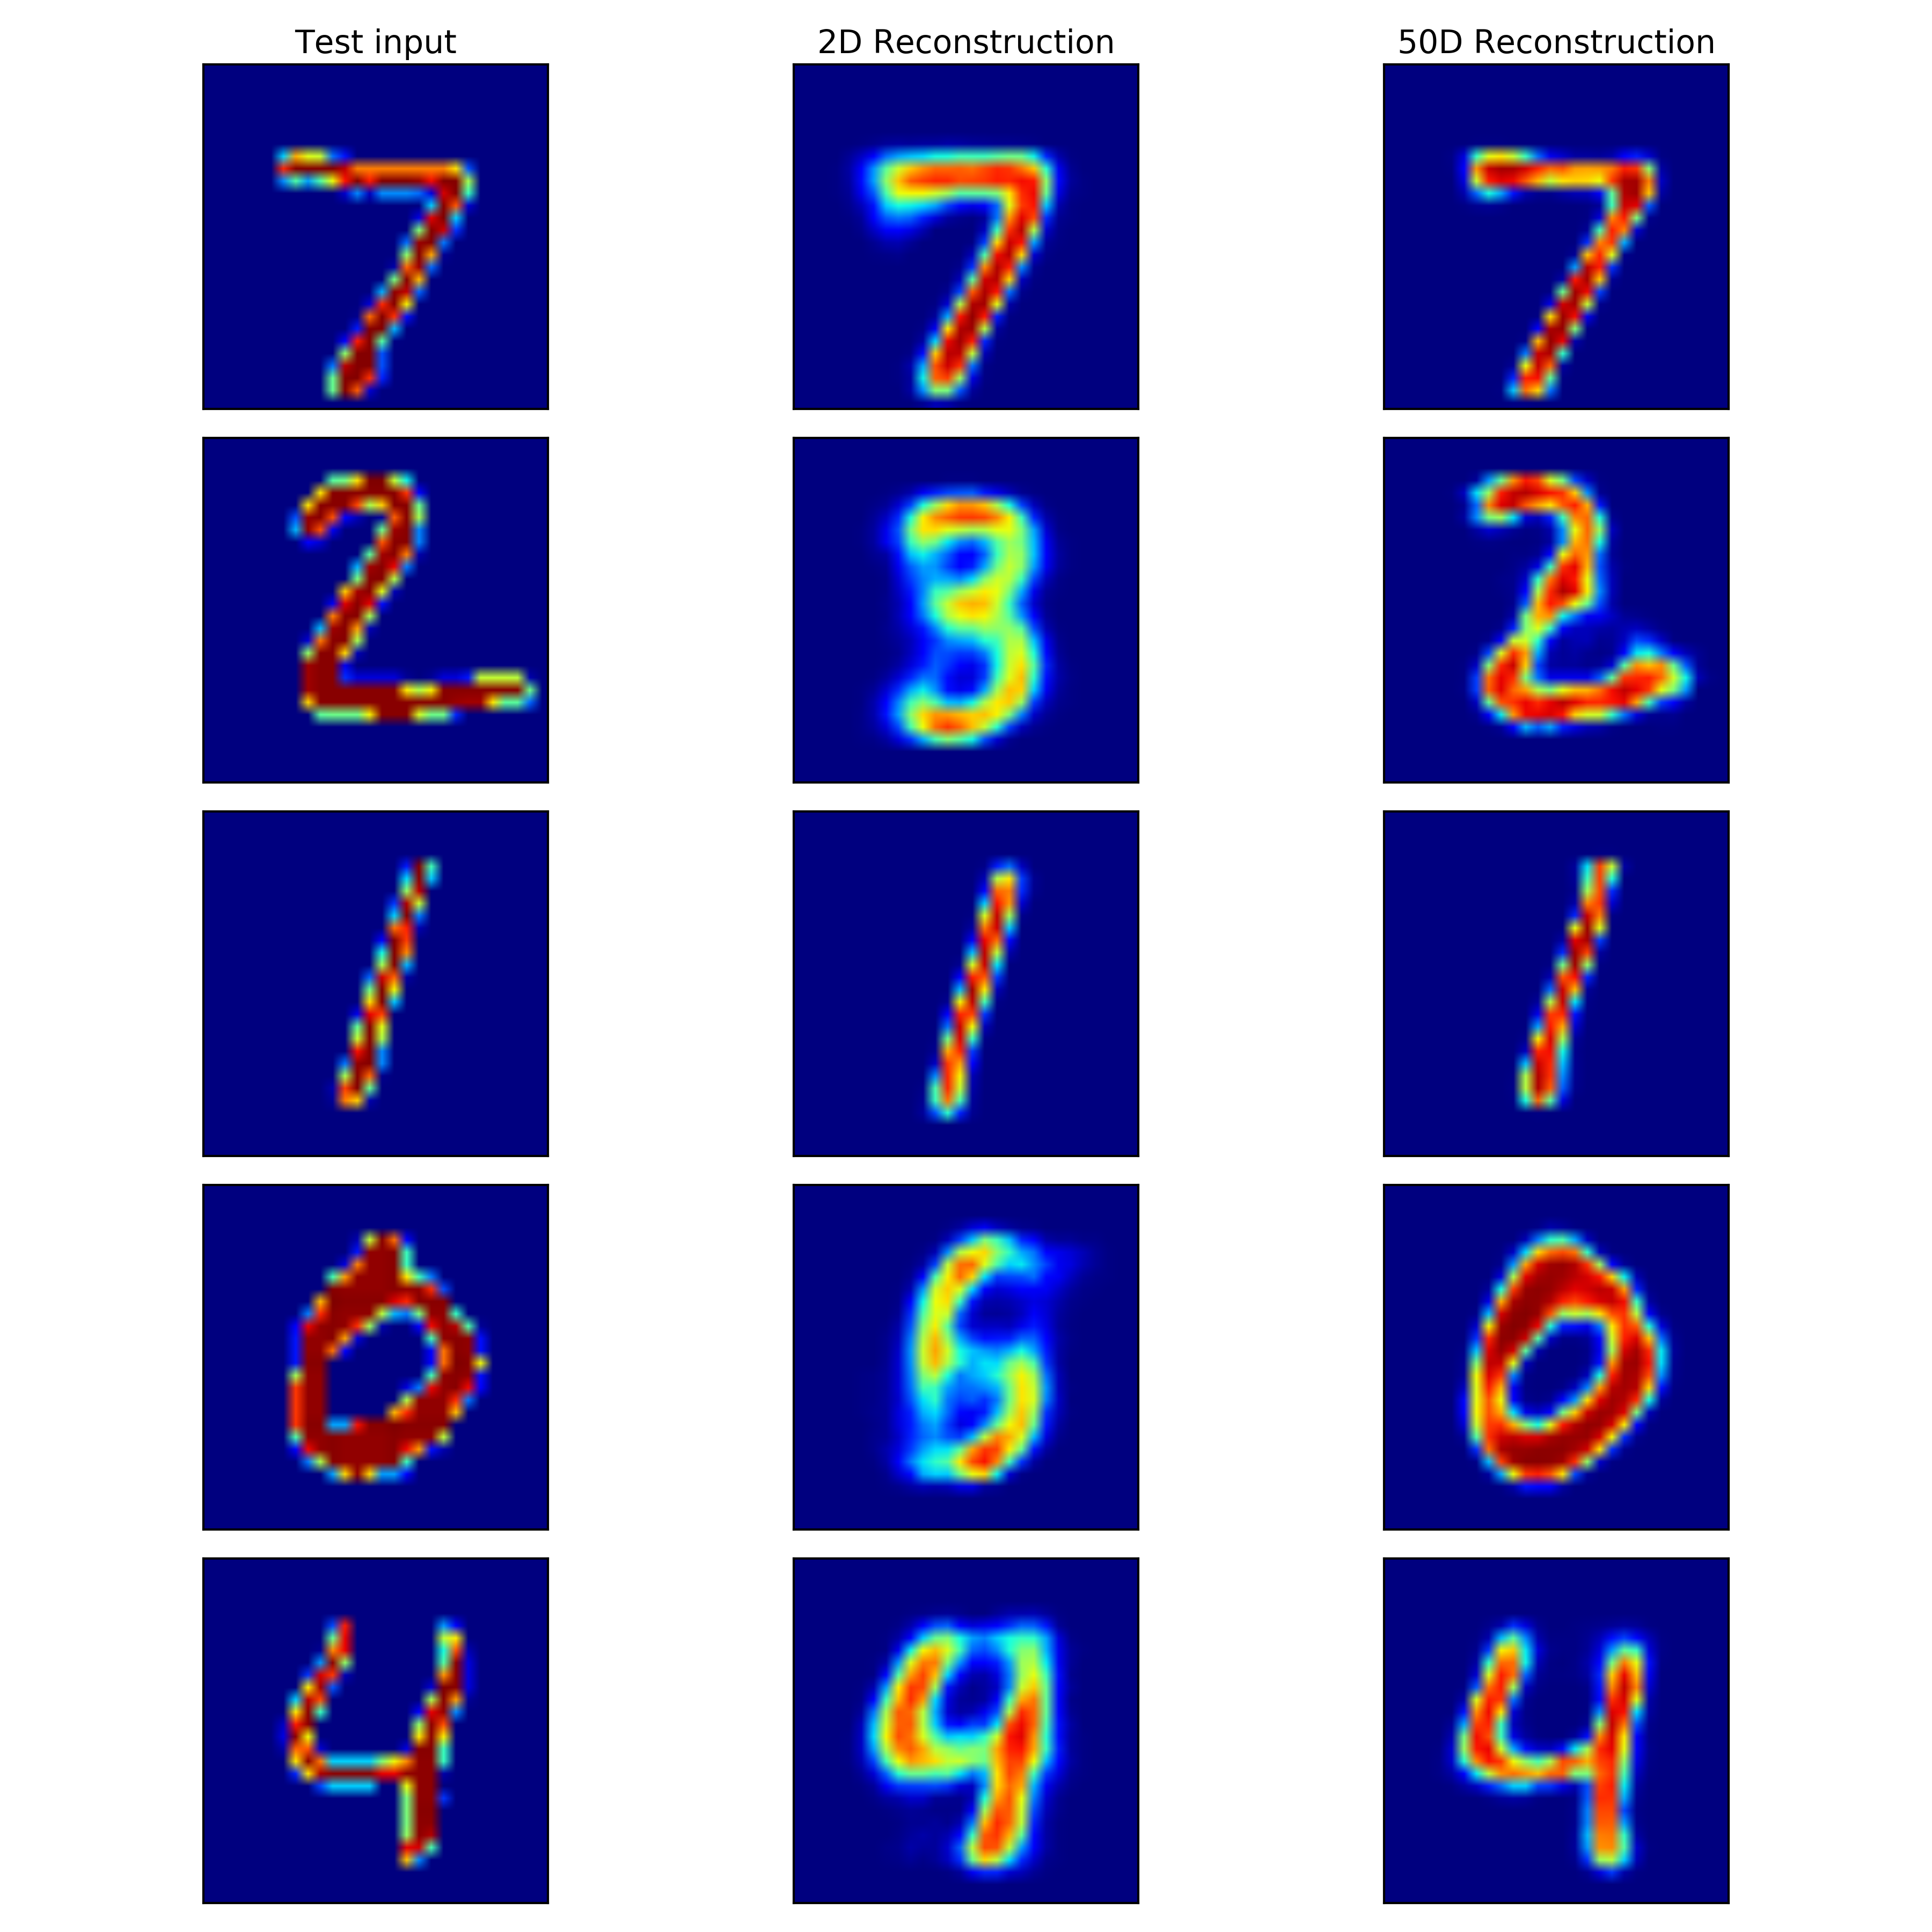
\includegraphics[scale=1]{{../plots/img/vis_recon}.png}}
    \caption{Reconstruction Visualization}
    \label{fig:recon}
  \end{minipage}
  \begin{minipage}[b]{0.45\textwidth}
    \resizebox{\linewidth}{!}{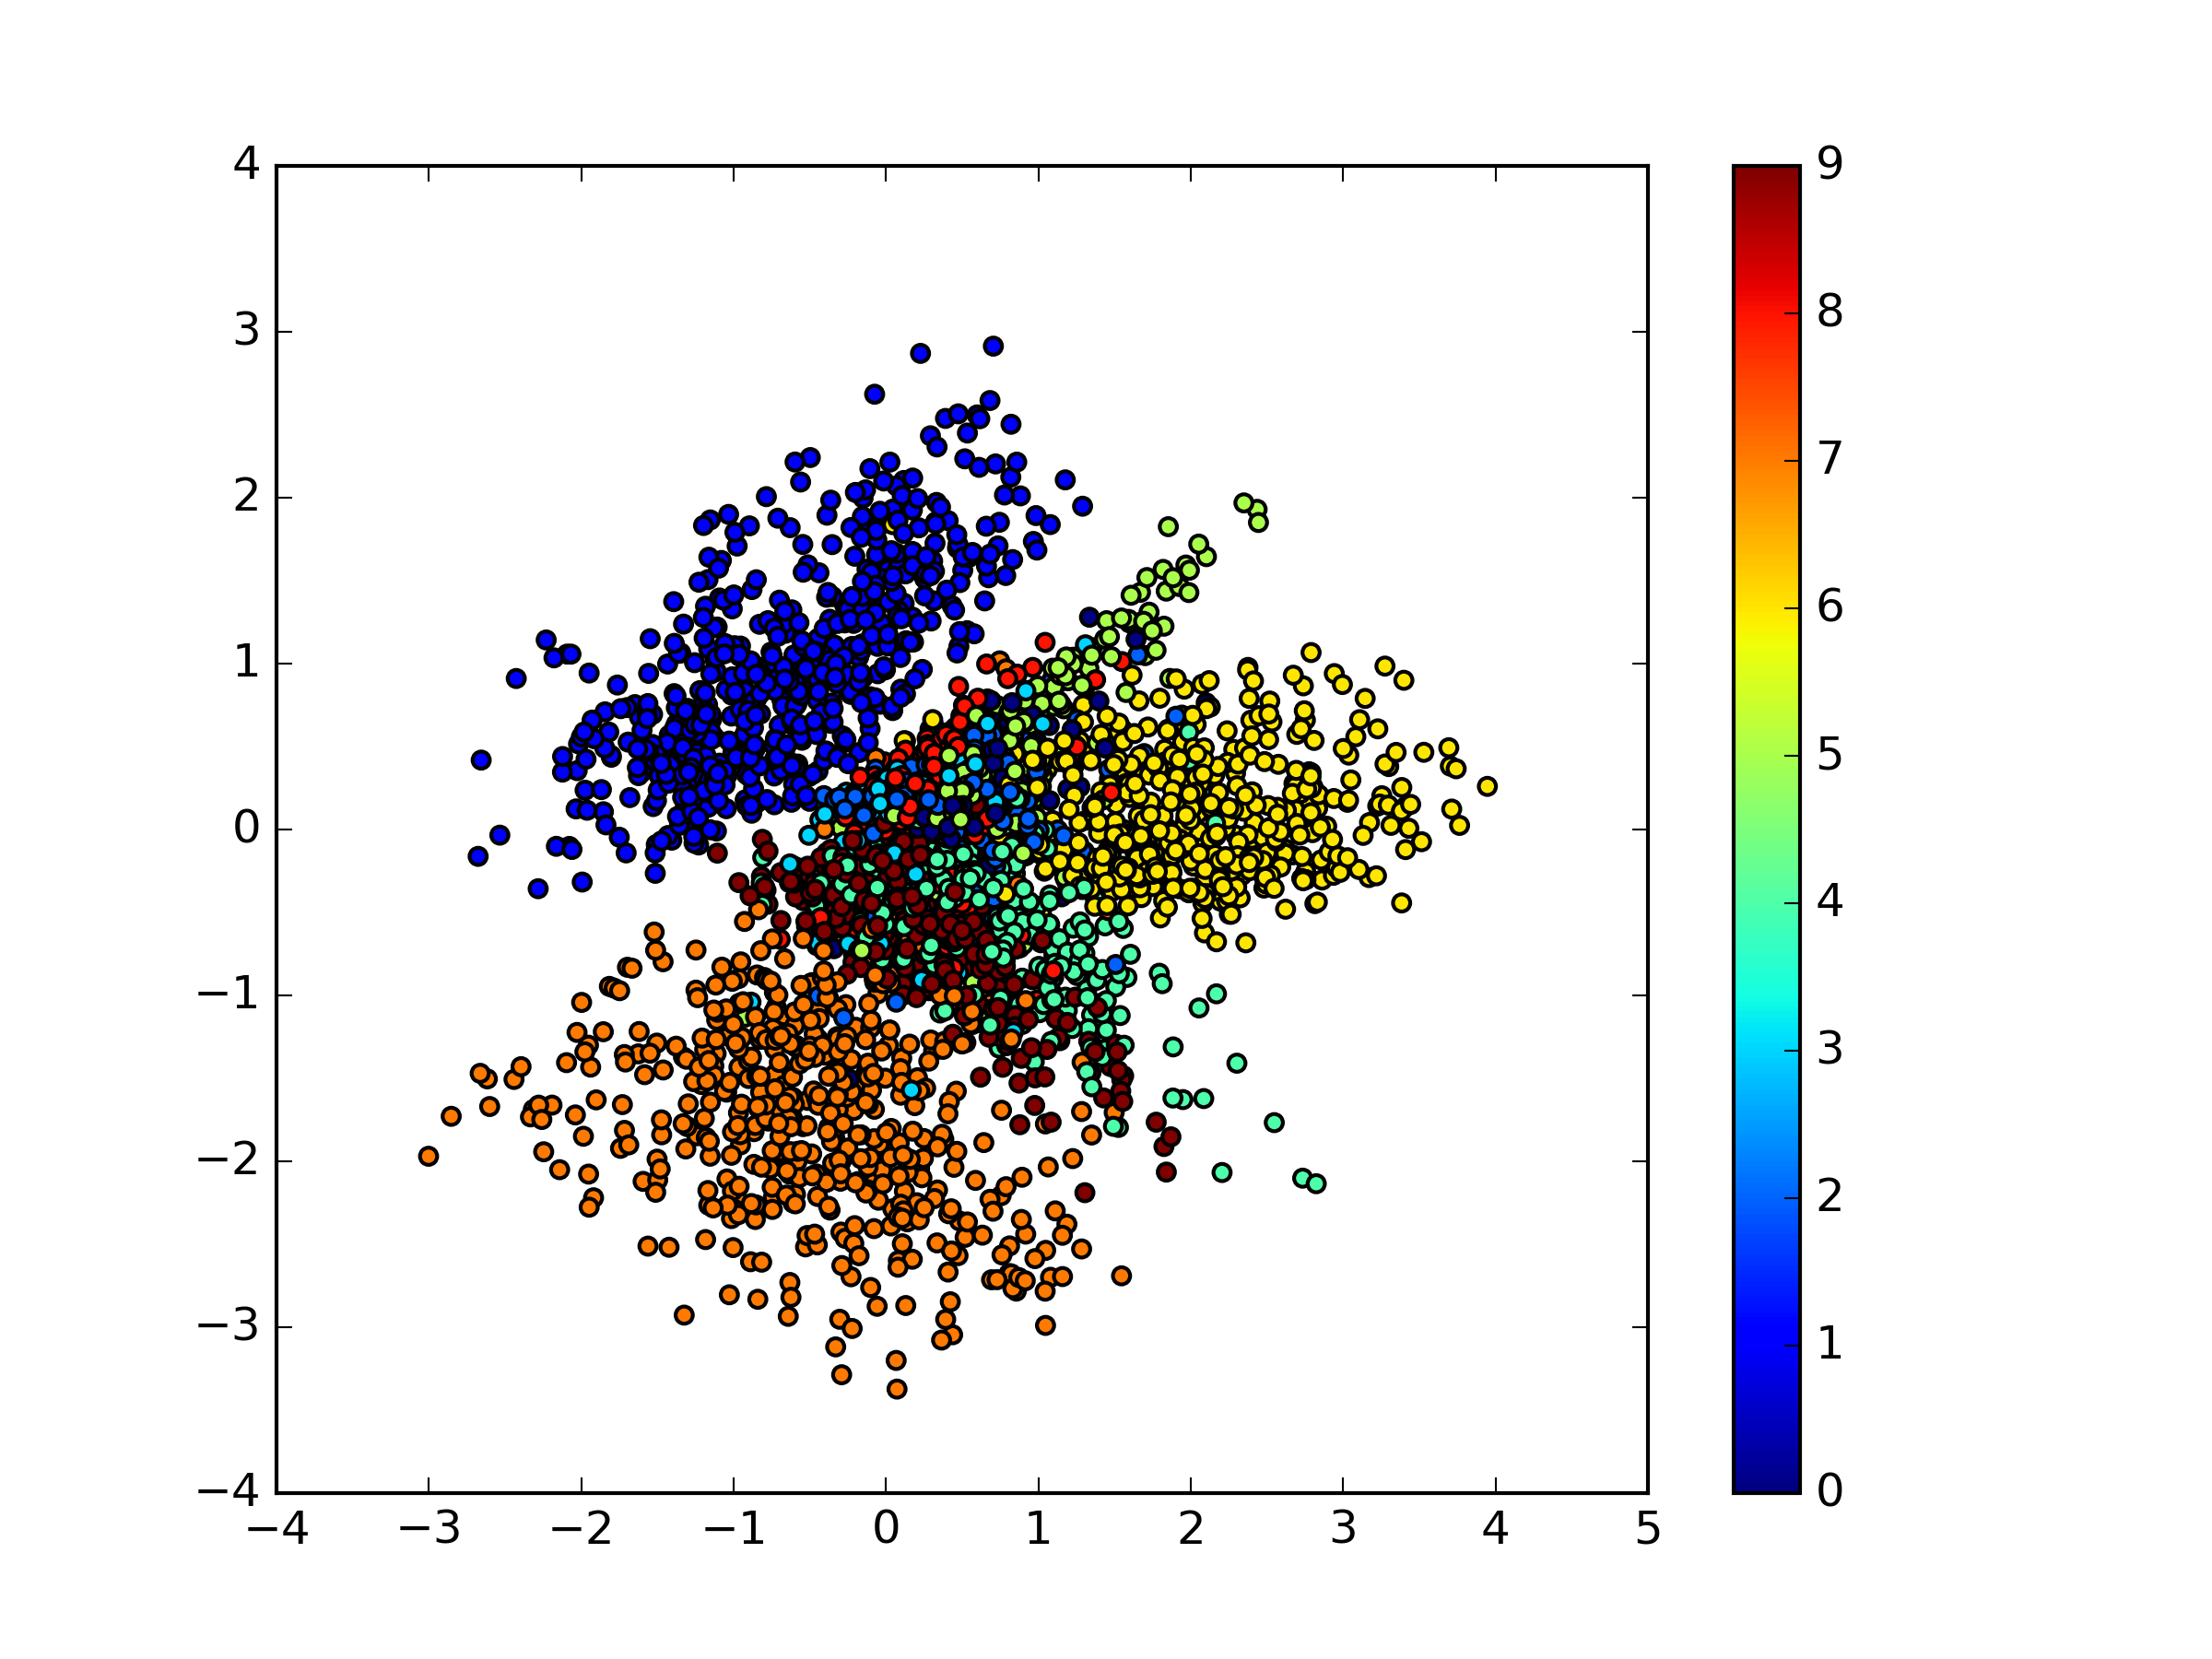
\includegraphics[scale=1]{{../plots/img/vis_scatter2}.png}}
    \caption{Data Encoding Visualization} 
    \label{fig:latenc}
  \end{minipage}
\end{figure}
\subsection{Latent Manifold Lattice Generation}
The final visualization technique utilizes just the decoder network of our VAE. To visualize our learned manifold we choose latent parameters on a lattice of a hyperplane of our latent space. Then we decode the values on our lattice and visualize the lattice in data space. See an example of this visualization in Figure \ref{fig:latlattice}. Notice that this manifold exactly corresponds to the encoding of our data classes into latent space, e.g. 6s at the top and 1s in the lower right. This is an extremely valuable visualization method because it illustrates how model transitions between data classes. Further, it accessibly demonstrates instances of problematic representation, such as the transition from 7s to 9s to 4s. This visualization technique demonstrates clearly how the latent space encodes representations of our data.
\section{Conclusion}
Our experiments show that the methods designed for improving deep variational auto encoders do not always provide significant improvements for shallow VAEs. Of the implementations we considered, the most important improvements came with correctly choosing the decoder distribution for our data type and optimizing with the importance weighted objective. We observed that additional latent dimensions improve the model up to a certain dimension, $n_z=10$, but further additional dimensions offer no benefit. To clarify this effect we consider the activity of those additional dimensions during training and observe that dimensions above the $10^{\text{th}}$ tend to be deactivated by being rendered unused during training. We assessed the effectiveness of our methods in maintaining active dimensions throughout training, particularly in reducing early pruning. As the literature suggested, implementing these methods did encourage greater dimension activity throughout training, which is an important characteristic when training deep VAEs. However, we found no significant correlation between increased latent dimension activity and improved learning in our shallow VAE. Finally, we demonstrated three visualization techniques for understanding the learned representation of our VAE. The three techniques each demonstrate, respectively, the entire VAE network, the encoder network, and the decoder network. 
\subsection{Further Research}
One direction for further research is to understand why the VAE deactivates dimensions above the $10^{\text{th}}$. It is suggestive since the MNIST data set is composed of exactly 10 classes. We might test this result by learning a subset of the MNIST classes, for example digits 1-5, and observing the effect on latent dimension activity. In general, we would explore the effect of our methods on more complex datasets, namely on continuous data. Finally, we would adjust our implementation to determine the effect of our methods on deep VAEs, confirming results from literature but  requiring more computational resources than were available here.

\bibliographystyle{plain}
\bibliography{bib}

\end{document}